% Options for packages loaded elsewhere
\PassOptionsToPackage{unicode}{hyperref}
\PassOptionsToPackage{hyphens}{url}
\documentclass[
  english,
]{article}
\usepackage{xcolor}
\usepackage{amsmath,amssymb}
\setcounter{secnumdepth}{5}
\usepackage{iftex}
\ifPDFTeX
  \usepackage[T1]{fontenc}
  \usepackage[utf8]{inputenc}
  \usepackage{textcomp} % provide euro and other symbols
\else % if luatex or xetex
  \usepackage{unicode-math} % this also loads fontspec
  \defaultfontfeatures{Scale=MatchLowercase}
  \defaultfontfeatures[\rmfamily]{Ligatures=TeX,Scale=1}
\fi
% \usepackage{lmodern}
\ifPDFTeX\else
  % xetex/luatex font selection
\fi
% Use upquote if available, for straight quotes in verbatim environments
\IfFileExists{upquote.sty}{\usepackage{upquote}}{}
\IfFileExists{microtype.sty}{% use microtype if available
  \usepackage[]{microtype}
  \UseMicrotypeSet[protrusion]{basicmath} % disable protrusion for tt fonts
}{}
\makeatletter
\@ifundefined{KOMAClassName}{% if non-KOMA class
  \IfFileExists{parskip.sty}{%
    \usepackage{parskip}
  }{% else
    \setlength{\parindent}{0pt}
    \setlength{\parskip}{6pt plus 2pt minus 1pt}}
}{% if KOMA class
  \KOMAoptions{parskip=half}}
\makeatother
\usepackage{color}
\usepackage{fancyvrb}
\newcommand{\VerbBar}{|}
\newcommand{\VERB}{\Verb[commandchars=\\\{\}]}
\DefineVerbatimEnvironment{Highlighting}{Verbatim}{commandchars=\\\{\}}
% Add ',fontsize=\small' for more characters per line
\newenvironment{Shaded}{}{}
\newcommand{\AlertTok}[1]{\textcolor[rgb]{1.00,0.00,0.00}{\textbf{#1}}}
\newcommand{\AnnotationTok}[1]{\textcolor[rgb]{0.38,0.63,0.69}{\textbf{\textit{#1}}}}
\newcommand{\AttributeTok}[1]{\textcolor[rgb]{0.49,0.56,0.16}{#1}}
\newcommand{\BaseNTok}[1]{\textcolor[rgb]{0.25,0.63,0.44}{#1}}
\newcommand{\BuiltInTok}[1]{\textcolor[rgb]{0.00,0.50,0.00}{#1}}
\newcommand{\CharTok}[1]{\textcolor[rgb]{0.25,0.44,0.63}{#1}}
\newcommand{\CommentTok}[1]{\textcolor[rgb]{0.38,0.63,0.69}{\textit{#1}}}
\newcommand{\CommentVarTok}[1]{\textcolor[rgb]{0.38,0.63,0.69}{\textbf{\textit{#1}}}}
\newcommand{\ConstantTok}[1]{\textcolor[rgb]{0.53,0.00,0.00}{#1}}
\newcommand{\ControlFlowTok}[1]{\textcolor[rgb]{0.00,0.44,0.13}{\textbf{#1}}}
\newcommand{\DataTypeTok}[1]{\textcolor[rgb]{0.56,0.13,0.00}{#1}}
\newcommand{\DecValTok}[1]{\textcolor[rgb]{0.25,0.63,0.44}{#1}}
\newcommand{\DocumentationTok}[1]{\textcolor[rgb]{0.73,0.13,0.13}{\textit{#1}}}
\newcommand{\ErrorTok}[1]{\textcolor[rgb]{1.00,0.00,0.00}{\textbf{#1}}}
\newcommand{\ExtensionTok}[1]{#1}
\newcommand{\FloatTok}[1]{\textcolor[rgb]{0.25,0.63,0.44}{#1}}
\newcommand{\FunctionTok}[1]{\textcolor[rgb]{0.02,0.16,0.49}{#1}}
\newcommand{\ImportTok}[1]{\textcolor[rgb]{0.00,0.50,0.00}{\textbf{#1}}}
\newcommand{\InformationTok}[1]{\textcolor[rgb]{0.38,0.63,0.69}{\textbf{\textit{#1}}}}
\newcommand{\KeywordTok}[1]{\textcolor[rgb]{0.00,0.44,0.13}{\textbf{#1}}}
\newcommand{\NormalTok}[1]{#1}
\newcommand{\OperatorTok}[1]{\textcolor[rgb]{0.40,0.40,0.40}{#1}}
\newcommand{\OtherTok}[1]{\textcolor[rgb]{0.00,0.44,0.13}{#1}}
\newcommand{\PreprocessorTok}[1]{\textcolor[rgb]{0.74,0.48,0.00}{#1}}
\newcommand{\RegionMarkerTok}[1]{#1}
\newcommand{\SpecialCharTok}[1]{\textcolor[rgb]{0.25,0.44,0.63}{#1}}
\newcommand{\SpecialStringTok}[1]{\textcolor[rgb]{0.73,0.40,0.53}{#1}}
\newcommand{\StringTok}[1]{\textcolor[rgb]{0.25,0.44,0.63}{#1}}
\newcommand{\VariableTok}[1]{\textcolor[rgb]{0.10,0.09,0.49}{#1}}
\newcommand{\VerbatimStringTok}[1]{\textcolor[rgb]{0.25,0.44,0.63}{#1}}
\newcommand{\WarningTok}[1]{\textcolor[rgb]{0.38,0.63,0.69}{\textbf{\textit{#1}}}}
\usepackage{longtable,booktabs,array}
\usepackage{caption}
\captionsetup[table]{skip=6pt}
\newcounter{none} % for unnumbered tables
\usepackage{calc} % for calculating minipage widths
% Correct order of tables after \paragraph or \subparagraph
\usepackage{etoolbox}
\makeatletter
\patchcmd\longtable{\par}{\if@noskipsec\mbox{}\fi\par}{}{}
\makeatother
% Allow footnotes in longtable head/foot
\IfFileExists{footnotehyper.sty}{\usepackage{footnotehyper}}{\usepackage{footnote}}
\makesavenoteenv{longtable}
\ifLuaTeX
\usepackage[bidi=basic,shorthands=off]{babel}
\else
\usepackage[bidi=default,shorthands=off]{babel}
\fi
\ifLuaTeX
  \usepackage{selnolig} % disable illegal ligatures
\fi
\setlength{\emergencystretch}{3em} % prevent overfull lines
\providecommand{\tightlist}{%
  \setlength{\itemsep}{0pt}\setlength{\parskip}{0pt}}
\usepackage[]{natbib}
\bibliographystyle{plainnat}
\makeatletter
\@ifpackageloaded{subcaption}{}{\usepackage{subcaption}}
\@ifpackageloaded{caption}{}{\usepackage{caption}}
\captionsetup[subfigure]{margin=0.5em}
\AtBeginDocument{%
\renewcommand*\figurename{Figure}
\renewcommand*\tablename{Table}
}
\AtBeginDocument{%
\renewcommand*\listfigurename{List of Figures}
\renewcommand*\listtablename{List of Tables}
}
\newcounter{pandoccrossref@subfigures@footnote@counter}
\newenvironment{pandoccrossrefsubfigures}{%
\setcounter{pandoccrossref@subfigures@footnote@counter}{0}
\begin{figure}\centering%
\gdef\global@pandoccrossref@subfigures@footnotes{}%
\DeclareRobustCommand{\footnote}[1]{\footnotemark%
\stepcounter{pandoccrossref@subfigures@footnote@counter}%
\ifx\global@pandoccrossref@subfigures@footnotes\empty%
\gdef\global@pandoccrossref@subfigures@footnotes{{##1}}%
\else%
\g@addto@macro\global@pandoccrossref@subfigures@footnotes{, {##1}}%
\fi}}%
{\end{figure}%
\addtocounter{footnote}{-\value{pandoccrossref@subfigures@footnote@counter}}
\@for\f:=\global@pandoccrossref@subfigures@footnotes\do{\stepcounter{footnote}\footnotetext{\f}}%
\gdef\global@pandoccrossref@subfigures@footnotes{}}
\@ifpackageloaded{float}{}{\usepackage{float}}
\floatstyle{ruled}
\@ifundefined{c@chapter}{\newfloat{codelisting}{h}{lop}}{\newfloat{codelisting}{h}{lop}[chapter]}
\floatname{codelisting}{Listing}
\newcommand*\listoflistings{\listof{codelisting}{List of Listings}}
\makeatother
\usepackage{bookmark}
\IfFileExists{xurl.sty}{\usepackage{xurl}}{} % add URL line breaks if available
\urlstyle{same}
% fallback for those not using the hyperref driver hyperxmp:
\makeatletter
\@ifundefined{xmpquote}{\newcommand{\xmpquote}[1]{#1}}{}
\makeatother
\hypersetup{
  pdftitle={A Living Meta-Analysis Architecture for Active Inference},
  pdfauthor={Daniel Friedman; Joel Dietz},
  pdflang={en},
  colorlinks=true,linkcolor=red,urlcolor=red,citecolor=red,anchorcolor=red,filecolor=red,
  pdfcreator={LaTeX via pandoc}}

\title{A Living Meta-Analysis Architecture for Active Inference}
\author{Daniel Friedman; Joel Dietz}
\date{}

\IfFileExists{seqsplit.sty}{\usepackage{seqsplit}}{\newcommand{\seqsplit}[1]{#1}}
\protected\def\breakseq#1{\seqsplit{#1}}
\protected\def\breaktt#1{\begingroup\ttfamily\seqsplit{#1}\endgroup}
\title{A Living Meta-Analysis Architecture for Active Inference}
\author{Daniel Friedman\\\footnotesize{Active Inference Institute}\\\footnotesize{\texttt{daniel@activeinference.institute}}\\\footnotesize{\href{https://orcid.org/0000-0001-6232-9096}{ORCID: 0000-0001-6232-9096}} \\and Joel Dietz\\\footnotesize{Massachusetts Institute of Technology (MIT)}\\\footnotesize{California Institute for Machine Consciousness (CIMC)}\\\footnotesize{\texttt{jdietz@mit.edu}}\\\footnotesize{\href{https://orcid.org/0000-0002-9456-2691}{ORCID: 0000-0002-9456-2691}} \\ \footnotesize{DOI: \href{https://doi.org/10.5281/zenodo.19461934}{10.5281/zenodo.19461934}}}
\date{\today}

% Core mathematics
\usepackage{amsmath}
\usepackage{amssymb}
\usepackage{amsfonts}
\usepackage{amsthm}

% Document layout
\usepackage[margin=1.8cm]{geometry}
\usepackage{float}
\usepackage{graphicx}
\usepackage[section]{placeins}  % Constrain floats to their section
\renewcommand{\floatpagefraction}{0.7}  % Require 70% fill for float-only pages
\renewcommand{\topfraction}{0.9}        % Allow large top floats

% Tables
\usepackage{booktabs}
\usepackage{longtable}
\usepackage{array}
\usepackage{multirow}

% Code listings
\usepackage{listings}

% Typography and formatting
\usepackage{microtype}
\usepackage{xcolor}

% Cross-references and citations (hyperref loaded by other packages with [unicode]; set options only)
\hypersetup{colorlinks=true,linkcolor=red,citecolor=red,urlcolor=red}
\usepackage[capitalise,noabbrev]{cleveref}
% NOTE: natbib is auto-injected by Pandoc via --natbib (which also writes
% \bibliographystyle{plainnat}). Do not re-declare \usepackage{natbib} here
% or LaTeX will error with "Option clash for package natbib".

% Figure caption formatting
\usepackage{caption}
\usepackage{subcaption}

% Algorithm typesetting
\usepackage[ruled,vlined]{algorithm2e}

% Custom commands for Active Inference notation
\newcommand{\FEP}{\textsc{fep}}
\newcommand{\AIF}{\textsc{aif}}
\newcommand{\KL}{\mathrm{KL}}
\newcommand{\E}{\mathbb{E}}
\newcommand{\F}{\mathcal{F}}

% NMF and topic modeling notation
\newcommand{\matW}{\mathbf{W}}  % NMF document-topic matrix
\newcommand{\matH}{\mathbf{H}}  % NMF topic-term matrix
\newcommand{\matV}{\mathbf{V}}  % NMF document-term matrix
\newcommand{\tfidf}{\text{TF-IDF}}
\newcommand{\cagr}{\text{CAGR}}
\newcommand{\score}{\operatorname{score}}
\newcommand{\corpusvar}[1]{\texttt{\{\{#1\}\}}}
\newcommand{\scoreH}[1]{\text{score}(H_{#1})}
\newcommand{\EBM}{\textsc{ebm}}
\newcommand{\VFE}{\mathcal{F}_{\text{VFE}}}
\newcommand{\RBM}{\textsc{rbm}}

% Assertion and evidence notation
\newcommand{\supports}{\mathrel{\text{supports}}}
\newcommand{\contradicts}{\mathrel{\text{contradicts}}}
\newcommand{\neutral}{\mathrel{\text{neutral}}}

% Domain taxonomy shorthands
\newcommand{\domA}{\text{A}}
\newcommand{\domB}{\text{B}}
\newcommand{\domC}{\text{C}}

% Expected free energy and growth metrics
\newcommand{\EFE}{\mathbf{G}}       % Expected free energy matrix
\newcommand{\doubling}{t_d}         % Doubling time
\newcommand{\meangrowth}{\bar{g}}   % Mean year-over-year growth rate

% Corpus and scoring notation
\newcommand{\Nstart}{N_{\text{start}}}  % Publication count in first year
\newcommand{\Nend}{N_{\text{end}}}      % Publication count in last year
\newcommand{\SH}{S(H)}                  % Supporting assertions for H
\newcommand{\CH}{C(H)}                  % Contradicting assertions for H
\newcommand{\AH}{A(H)}                  % All assertions for H

% Tool and project shorthands
\newcommand{\nanopub}{\textsc{np}}      % Nanopublication shorthand
\newcommand{\ollama}{\textsc{Ollama}}   % Ollama LLM server
\newcommand{\pymdp}{\textsc{pymdp}}     % pymdp library

% Network and graph operators
\DeclareMathOperator{\PageRank}{PageRank}  % PageRank operator
\newtheorem{theorem}{Theorem}[section]
\newtheorem{remark}[theorem]{Remark}
\newtheorem{example}[theorem]{Example}

\begin{document}
\begin{titlepage}
\centering
\vspace*{2cm}
{\LARGE\bfseries A Living Meta-Analysis Architecture for Active Inference\par}
\vspace{0.75em}
{\large Assertion Extraction, Nanopublications, and Hypothesis Scoring\par}
\vfill
\makeatletter
{\@author\par}
\vspace{1em}
{\@date\par}
\makeatother
\vfill
\end{titlepage}
\thispagestyle{empty}
\tableofcontents
\newpage

\section{Abstract}\label{abstract}

\begin{quote}
\textbf{Snapshot status:} 2026-07-26 snapshot; source gate blocked;
1071/1071 eligible papers processed; 2,561 assertions; PDF and HTML
pass. Source status: arXiv complete; Semantic Scholar incomplete
(HTTPError); OpenAlex complete. The current year is treated as YTD /
partial year and is excluded from the CAGR endpoint when incomplete. The
configured model is \texttt{gemma3:4b} with pipeline 2.0.6 and prompt
v2.0.6. Scores are evidence mapping and hypothesis triage, not
scientific confirmation.
\end{quote}

No prior automated system tracks hypothesis-level evidence mapping
across the configured Active Inference and Free Energy Principle (FEP)
search scope. Manual synthesis cannot keep pace with a field that has
grown at a compound annual rate of 24.94\% across 2000--2026 (empirical
publication span 2003--2026), and the FEP's theoretical generality has
invited falsifiability critiques that only hypothesis-specific triage
can address. Building on pioneering systematic manual annotation paired
with ontology-based analysis at the scale of hundreds of papers, we
present a computational meta-analysis framework that automates and
scales this approach. The configured retrieval sources are arXiv,
Semantic Scholar, and OpenAlex; for this snapshot, arXiv, OpenAlex
completed; Semantic Scholar incomplete. The retained corpus contains
\(N = 1106\) papers (inclusion from 2000 onward), deduplicated via a
canonical identifier hierarchy (DOI \(>\) arXiv ID \(>\) Semantic
Scholar ID \(>\) OpenAlex ID). It classifies papers into a three-tier
taxonomy spanning eight categories: A (Core Theory), B (Tools \&
Translation), and C (Application Domains). An LLM-powered extraction
system evaluates each abstract against eight core hypotheses, separating
(1) explicit source claims, (2) whether the abstract supplies evidence,
and (3) pipeline hypothesis triage---each encoded in structured
nanopublications with full extraction provenance.

All extracted assertions are machine-generated; hypothesis scores report
citation-weighted evidence mapping and triage, not scientific
confirmation. In the absence of a human-annotated gold set, a stratified
agreement study (\(n = 256\)) compares pipeline triage against an
independent, deterministic keyword-rule reference: pipeline precision
0.013 and recall 1.000 against the rule reference, with
reference--pipeline direction agreement of only \(\kappa = -0.048\). The
low agreement limits interpretation of every derived score; rankings and
trajectories are presented as descriptive summaries, not validated
scientific estimates. Human gold-standard validation remains future
work.

The resulting evidence landscape reveals a field where application
domains (Domain C, 61.3\%) collectively dominate the corpus, with tools
development (Domain B, 23.8\%) and core theory (Domain A, 14.9\%)
rounding out the taxonomy. Non-negative matrix factorization identifies
8 latent topics that cross-cut the keyword taxonomy, and citation
network analysis exposes a sparse yet structured graph (4,829
intra-corpus edges out of 46,598 total outgoing
references---\textbf{only 10.4\% reference resolution}) anchored by
pronounced hub papers. Hypothesis triage scores are shown in descriptive
tiers for comparison; absolute magnitudes are affected by publication
selection and linguistic asymmetry, and the robustness of the rankings
and trajectories remains unvalidated. This work provides a reusable
architecture for \emph{living literature reviews}---continuously updated
knowledge graphs that map citation-weighted evidence and support
hypothesis triage across rapidly evolving fields.

\textbf{Keywords:} Active Inference, Free Energy Principle,
meta-analysis, knowledge graph, nanopublications, bibliometrics,
hypothesis scoring, LLM extraction, computational neuroscience

\newpage

\section{Introduction: Evidence Gaps in a Rapidly Expanding
Field}\label{introduction-evidence-gaps-in-a-rapidly-expanding-field}

\subsection{The Free Energy Principle and Active Inference
Framework}\label{the-free-energy-principle-and-active-inference-framework}

The Free Energy Principle (FEP), introduced by Karl Friston, proposes
that self-organizing systems maintain their structural and functional
integrity by minimizing variational free energy---an upper bound on
sensory surprise \citep{friston2006free, friston2010free}. Under this
principle, living systems are cast as approximate Bayesian inference
engines that build generative models of their environment and act to
reduce the discrepancy between predicted and observed states. Active
Inference (AIF) extends this picture from passive perception to
goal-directed behavior: agents select actions that bring about
observations consistent with their preferred states, unifying
perception, learning, and decision-making within a single variational
framework \citep{parr2022active, friston2017active}. Since its initial
formulation for sensorimotor control, AIF has been applied to
navigation, visual foraging, language comprehension, social cognition,
and multi-agent coordination. Bayesian mechanics
\citep{sakthivadivel2023bayesian} has further strengthened the
mathematical foundations of the FEP by grounding Markov blanket dynamics
in the physics of belief-based systems, placing the principle on a
footing commensurate with established physical theories. Importantly,
the variational free energy minimization at the core of the FEP shares
deep mathematical connections with the broader family of Energy-Based
Models (EBMs) \citep{lecun2006tutorial}---including Helmholtz machines
\citep{dayan1995helmholtz}, Boltzmann machines
\citep{hinton2002training}, and variational autoencoders
\citep{kingma2014auto}---all of which parameterize learning and
inference through scalar energy functions and variational bounds. This
convergence motivates the inclusion of EBM-adjacent literature in our
search scope.

\subsection{Challenges Posed by Rapid Literature
Growth}\label{challenges-posed-by-rapid-literature-growth}

The active inference literature has grown at a compound annual rate of
24.94\% across 2003--2026, with annual output accelerating sharply after
2013. While early research concentrated on theoretical neuroscience, the
field has since diversified across biology (C5), robotics (C2),
computational psychiatry (C4), algorithm scaling (B), and formal
mathematics (A1). With \(N = 1106\) papers spanning 8 categories across
3 domains, no prior automated system tracks hypothesis-level evidence
across the full corpus. This creates three interrelated challenges.
First, the balance of evidence for core claims---such as FEP
universality or the physical realism of Markov blankets---cannot be
assessed without structured, hypothesis-specific extraction at corpus
scale. Second, because the relationship between mathematical formalisms
and empirical evidence is frequently implicit, systematic evidence
synthesis demands substantial manual effort: Knight et
al.~\citep{knight2022fep} required human annotators to manually code
hundreds of papers. Third, new entrants must navigate a literature
weighted toward broad qualitative philosophy (A2), interspersed with
specialized applied subfields whose findings are difficult to locate
without domain-specific search strategies.

Traditional narrative reviews attempt to address these challenges but
are static, subjective, and quickly outdated. Systematic reviews from
evidence-based medicine offer rigorous aggregation but are structured
for clinical trial data with homogeneous outcome measures, making them
poorly suited for the heterogeneous ontological and computational claims
in this literature. The expansion of predictive processing
\citep{clark2013whatever, hohwy2013predictive} and the emergence of
Bayesian mechanics \citep{sakthivadivel2023bayesian} further broaden the
scope of assertions that a comprehensive meta-analysis must reconcile.
Critically, the falsifiability of the FEP itself remains contested
\citep{colombo2021free}: because free energy minimization can be
reframed to accommodate any behavior post hoc, distinguishing genuine
predictive commitment from tautological redescription requires exactly
the hypothesis-specific, evidence-quantified framework we propose here.

\subsection{Related Work and Prior
Meta-Analyses}\label{related-work-and-prior-meta-analyses}

Several prior efforts have surveyed aspects of the Active Inference
landscape. Sajid et al.~\citep{sajid2021active} compare active inference
with alternative decision-making frameworks; Da Costa et
al.~\citep{dacosta2020active} synthesize the discrete-state-space
formulation; Lanillos et al.~\citep{lanillos2021active} survey robotics
applications; Smith et al.~\citep{smith2021computational} provide a
tutorial bridging theory and empirical data; and Millidge et
al.~\citep{millidge2021understanding} examine information-theoretic
foundations of exploration behavior. Ramstead et
al.~\citep{ramstead2018answering} extend the FEP to questions of
biological self-organization, while Pezzulo et
al.~\citep{pezzulo2015active} connect active inference to homeostatic
regulation. Millidge \citep{millidge2024retrospective} provides a
practitioner's retrospective confirming that AIF's strongest
demonstrated results arise from novel discrete generative models, while
scalability relative to deep reinforcement learning remains the field's
central open challenge.

Parallel to these synthesis efforts, Sanjeev V. Namjoshi's 2026
textbook, \emph{Fundamentals of Active Inference}
\citep{namjoshi2026fundamentals}, provides a comprehensive,
computationally explicit foundation for the field designed for
engineers. In conjunction with this text, Namjoshi developed the
\texttt{aif-fep-db} repository \citep{namjoshi2026aiffepdb}---an
open-source, dynamically updated database of scraped and tagged
publications covering active inference, the free energy principle, and
predictive processing. While \texttt{aif-fep-db} curates and categorizes
the literature to facilitate reproducible systematic reviews and
interactive Dash-based exploration, it functions primarily as a modular
bibliographic foundation rather than an automated hypothesis evaluation
engine.

Closest to our work, Knight, Cordes, and Friedman \citep{knight2022fep}
conducted a systematic literature analysis of publications using the
terms ``Free Energy Principle'' or ``Active Inference,'' with an
emphasis on works by Karl J. Friston. Their analysis---maintained by the
Active Inference Institute---combined manual annotation of structural,
visual, and mathematical features with automated analyses using the
Active Inference Ontology at the scale of thousands of citations and
hundreds of annotated papers. That study identified six development
directions---including broader scope, richer annotation, and
transferable approaches---and represents an important precursor to
automated meta-analysis of this field.

These prior works differ from the present study along four dimensions.
First, \textbf{scale}: narrative reviews cover tens to low hundreds of
papers; our pipeline processes \(N = 1106\). Second, \textbf{structure}:
prior reviews produce prose summaries rather than machine-queryable
knowledge graphs with typed relationships. Third, \textbf{temporal
tracking}: no prior system computes how evidence for specific hypotheses
evolves year over year. Fourth, \textbf{automation}: the systematic
analysis of Knight et al.~\citep{knight2022fep} pioneered quantitative
literature analysis but relied on manual annotation, limiting update
frequency. Our framework advances this line of work by (1) fully
automating assertion extraction via LLM-based hypothesis scoring, (2)
constructing a structured, RDF-compatible knowledge graph scored by
citation-weighted evidence, and (3) tracking how evidence for core
claims evolves over time through temporal trend analysis.

\subsection{Synergizing Knowledge Graphs and
LLMs}\label{synergizing-knowledge-graphs-and-llms}

Broadening this synthesis, recent systematic literature initiatives
underscore a powerful reciprocal synergy between Large Language Models
(LLMs) and Knowledge Graphs: LLMs parse unstructured text to rapidly
extract semantic claims, efficiently populating the structured,
queryable architecture of the graph
\citep{quevedo2025combining, li2024unifying}. We adopt the
\emph{nanopublication} \citep{groth2010anatomy}---a minimal,
machine-readable unit of scientific evidence comprising a core assertion
bound to explicit provenance metadata---as the fundamental serialization
format for this extracted knowledge.

\subsection{This Study: Approach and
Overview}\label{this-study-approach-and-overview}

This paper presents a computational meta-analysis of the Active
Inference literature (\(N = 1106\)). Rather than relying exclusively on
bibliometric metadata or slow manual coding, we deploy a Large Language
Model (LLM) to ``read'' each paper's abstract and assess its
relationship to eight core hypotheses within the FEP paradigm. We
serialize these assessments as nanopublications---each encoding an
assertion (``Paper X supports Hypothesis Y'') coupled with the LLM's
natural-language reasoning and confidence score. The resulting knowledge
graph aggregates these nanopublications and links them to paper
metadata, citation networks, subfield classifications, and hypothesis
definitions. A citation-weighted scoring formula quantifies the net
evidence for or against each hypothesis, producing scores in \([-1, 1]\)
that reflect both the direction and strength of published evidence.
Importantly, this represents an open-source introductory analysis which
will be augmented and extended, and stewarded in collaborative
development by the Active Inference Institute (activeinference.org).

\subsection{Research Questions}\label{research-questions}

This meta-analysis addresses four primary research questions:

\begin{enumerate}
\def\labelenumi{\arabic{enumi}.}
\tightlist
\item
  \textbf{RQ1 (Field Structure):} What is the disciplinary structure and
  growth trajectory of the Active Inference literature, and how are
  papers distributed across the three domains---Core Theory (A), Tools
  \& Translation (B), and Application Domains (C)? We expect Domain A to
  dominate but anticipate measurable diversification into applied
  domains.
\item
  \textbf{RQ2 (Growth Dynamics):} What are the temporal growth dynamics
  of the field, and which subfields are experiencing the most rapid
  expansion? Prior reviews suggest accelerating growth post-2013; we
  quantify this trajectory and identify which application domains drive
  it.
\item
  \textbf{RQ3 (Hypothesis Evidence):} What is the current balance of
  evidence for and against the eight standard hypotheses, and how has
  this balance evolved over time? We expect well-established hypotheses
  (H4 Predictive Coding) to show consensus while philosophically
  contested claims (H3 Markov Blanket Realism) show mixed evidence. (See
  hypothesis dashboard and assertion figures in the
  \hyperref[sec:hypothesis_results]{hypothesis results}.)
\item
  \textbf{RQ4 (Tooling Readiness):} What is the state of software
  tooling and infrastructure for Active Inference research, and what
  gaps remain? We survey available implementations to identify whether
  the ecosystem is fragmented or converging.
\end{enumerate}

\subsection{Scope and Delimitations}\label{scope-and-delimitations}

This study focuses on the English-language peer-reviewed and preprint
literature retrievable from arXiv, Semantic Scholar, and OpenAlex. Our
search scope begins at 2003---chosen to capture Energy-Based Model and
variational Bayesian antecedents (Helmholtz machines, VAEs, early
Bayesian brain formulations
\citep{dayan1995helmholtz, lecun2006tutorial}) that share deep
mathematical foundations with variational free energy minimization and
predated the Free Energy Principle label introduced in 2006
\citep{friston2006free}. The scope includes both the core Active
Inference and Free Energy Principle literature and adjacent Energy-Based
Model research where it intersects with variational inference or
generative modeling---capturing the growing convergence between these
traditions. We do not include book chapters or monographs not indexed by
these sources, software documentation, or non-English publications.
Domain classification uses keyword matching (200+ indicators across 8
categories) rather than expert annotation---a deliberate trade-off
favoring reproducibility over precision, whose consequences we quantify
in the \hyperref[sec:field_overview]{field overview}. Hypothesis scoring
relies on LLM-extracted assertions operating on abstracts only; claims
embedded in method sections, discussion paragraphs, or supplementary
materials are not captured, and the fraction of relevant evidence
residing in these sections is unknown. The fidelity and limitations of
abstract-only extraction are examined in the
\hyperref[sec:extraction_pipeline]{extraction pipeline section}. The
hypothesis definitions and domain taxonomy are informed by, but not
identical to, the Active Inference Ontology used by Knight et
al.~\citep{knight2022fep}; future alignment would enable direct
comparison with that earlier analysis.

\subsection{Principal Contributions}\label{principal-contributions}

This work makes five contributions:

\begin{enumerate}
\def\labelenumi{\arabic{enumi}.}
\item
  \textbf{A multi-source retrieval and deduplication pipeline} for
  Active Inference literature, using a canonical identifier hierarchy
  across three academic databases.
\item
  \textbf{A nanopublication-based knowledge graph schema} encoding
  directed, confidence-scored assertions about eight core hypotheses
  with full provenance tracking.
\item
  \textbf{A quantitative field overview} characterizing the growth,
  domain distribution (A/B/C taxonomy), citation topology, and latent
  topic structure of the Active Inference literature, with specific
  attention to how recent benchmark results
  (\hyperref[sec:subfield_analyses]{detailed in the domain analyses})
  are reshaping the scalability and application landscape.
\item
  \textbf{An LLM-based hypothesis scoring dashboard} that produces
  differentiated evidence profiles with temporal trend visualization.
\item
  \textbf{A tooling assessment} of the software ecosystem supporting
  Active Inference research, including the implemented extraction
  pipeline, existing software (pymdp, SPM, RxInfer.jl), and knowledge
  graph infrastructure.
\end{enumerate}

The remainder of this paper is organized as follows.
\hyperref[sec:methods]{The methodology section} describes the end-to-end
pipeline---the central contribution enabling reproducible, automated
evidence synthesis---with separate treatments of
\hyperref[sec:methods_retrieval]{literature retrieval},
\hyperref[sec:extraction_pipeline]{LLM-based assertion extraction},
\hyperref[sec:methods_bibliometrics]{bibliometric analysis}, the
\hyperref[sec:methods_kg]{nanopublication-based knowledge graph}, and
\hyperref[sec:methods_viz]{visualization, validation, and variable hydration}.
\hyperref[sec:hypothesis_results]{The hypothesis evidence landscape}
presents quantitative scoring results (RQ3), followed by
\hyperref[sec:field_overview]{the field overview} with domain-level
analysis (RQ1, RQ2),
\hyperref[sec:subfield_analyses]{detailed domain analyses},
\hyperref[sec:text_analytics]{text analytics}, and
\hyperref[sec:citation_network]{citation network topology}.
\hyperref[sec:conclusion]{The conclusion} addresses limitations and
future directions; the \hyperref[sec:discussion]{discussion} provides
community recommendations and open questions. Appendix
\ref{sec:technical_appendix} collects mathematical and algorithmic
details; Appendix \ref{sec:tooling} surveys the tooling landscape (RQ4).

\newpage

\section{Methodology: Pipeline Design and Formal
Definitions}\label{sec:methods}

This section describes the end-to-end computational meta-analysis
pipeline. Each stage corresponds to a tested, independently executable
script that reads upstream outputs and produces structured artifacts.
The pipeline extends the systematic literature analysis approach of
Knight et al.~\citep{knight2022fep}---which combined manual annotation
with ontology-based automated analysis---by substituting manual coding
with fully automated, LLM-driven assertion extraction and
citation-weighted hypothesis scoring. All code, configuration files, and
reproducibility instructions are available in the public
\href{https://github.com/ActiveInferenceInstitute/act_inf_metaanalysis}{Active
Inference Institute meta-analysis repository}
(\breaktt{ActiveInferenceInstitute/act\_inf\_metaanalysis}); dependencies
are pinned and managed with \texttt{uv} for reproducible local
execution.

\subsection{Pipeline Overview}\label{pipeline-overview}

The retrieval, analysis, extraction, visualization, validation,
hydration, and rendering stages are summarized in
\Cref{tab:pipeline_stages}.

\begin{table}[htbp]
\centering
\caption{Nine-stage computational meta-analysis pipeline. Stages 1--5 generate the publication content; stages 6--9 provide full-text QA, deterministic validation, cross-artifact validation, and manifest closure. Each stage is independently executable and reads upstream outputs to produce structured artifacts.}
\label{tab:pipeline_stages}
\begin{tabular}{cllll}
\toprule
\textbf{Stage} & \textbf{Script} & \textbf{Primary Input} & \textbf{Primary Output} & \textbf{Section} \\
\midrule
1 & \breaktt{01\_literature\_search.py} & API queries & \texttt{corpus.jsonl} & \hyperref[sec:methods_retrieval]{Retrieval} \\
2 & \breaktt{02\_meta\_analysis\_pipeline.py} & \texttt{corpus.jsonl} & Classification, temporal, TF-IDF, NMF, citation network JSONs & \hyperref[sec:methods_bibliometrics]{Bibliometrics} \\
3 & \breaktt{03\_build\_knowledge\_graph.py} & \texttt{corpus.jsonl} & \breaktt{nanopublications.jsonl}, \breaktt{nanopublications.trig}, scores & \hyperref[sec:methods_kg]{Knowledge Graph} \\
4 & \breaktt{04\_generate\_figures.py} & All Stage 2--3 JSONs & 16 publication-ready PNGs & \hyperref[sec:methods_viz]{Visualization} \\
5 & \breaktt{z\_generate\_manuscript\_variables.py} & All output JSONs & Rendered manuscript Markdown & \hyperref[sec:methods_viz]{Injection} \\
6 & \breaktt{06\_fulltext\_assessment.py} & \texttt{corpus.jsonl} & Full-text availability report & QA \\
7 & \breaktt{07\_run\_validation\_study.py} & Nanopubs + corpus & Rule-reference agreement metrics & Validation \\
8 & \breaktt{08\_validate\_artifacts.py} & All current artifacts & Cross-artifact contract report & Validation \\
9 & \breaktt{09\_write\_pipeline\_manifest.py} & Inputs + gate reports & Hashes, counts, versions, gate results & Provenance \\
\bottomrule
\end{tabular}
\end{table}

Scripts act as thin orchestrators that import methods from tested
library modules and handle file I/O. All computation resides in the
\texttt{src/} packages; no analysis logic is embedded in scripts.
End-to-end pipeline execution completes in under one hour on commodity
hardware (excluding LLM extraction, which depends on model size and
inference backend); all stochastic components use fixed random seeds for
deterministic reproduction.

\subsection{Reproducible Build
Infrastructure}\label{reproducible-build-infrastructure}

The analysis pipeline described above is embedded within
\texttt{template/}
\citep{Friedman2026TemplateReproducibleGenerative, FriedmanTemplateSoftware},
an open-source Infrastructure-as-Code system for computational research
that turns a full research compendium---code, data, tests, manuscript,
and provenance---into a single, version-controlled, deterministically
buildable repository with an enforced, test-gated publication pipeline.
\texttt{template/} applies the principle of Infrastructure as Code to
the research lifecycle, making the manuscript, test suite, and
provenance chain independently verifiable. The system operationalizes
FAIR4RS principles \citep{wilkinson2016fair} and supply-chain-style
provenance for manuscripts, targeting structural causes of the
reproducibility crisis: fragmented workflows across LaTeX, notebooks,
and ad-hoc scripts, lack of end-to-end testing, and no binding between
code, data, figures, and the final PDF.

The system employs a Two-Layer Architecture: a globally shared
\emph{infrastructure layer} provides generic services---logging,
rendering, validation, reporting, and LLM integration---while
self-contained \emph{project workspaces} carry their own
\texttt{manuscript/}, \texttt{scripts/}, \texttt{src/}, \texttt{tests/},
\texttt{data/}, and \texttt{output/} directories. The tested build runs
analysis, deterministic validation, PDF/HTML rendering, and output
validation. A Zero-Mock testing policy requires tests to exercise real
filesystem operations, real subprocess calls, and real computation.
Cryptographic provenance is recorded in generated artifacts, and the
\texttt{template/} framework supplies the shared rendering and
validation methods. The project is available under the MIT License at
\breaktt{https://github.com/ActiveInferenceInstitute/act\_inf\_metaanalysis}.

\newpage

\subsection{Stage 1: Multi-Source Literature Retrieval and
Deduplication}\label{sec:methods_retrieval}

We retrieve papers from three complementary academic databases to
maximize coverage and enable cross-source deduplication. The retrieval
window begins at 2003, encompassing the period when Energy-Based Model
and variational Bayesian research
\citep{dayan1995helmholtz, lecun2006tutorial} provided mathematical
precursors to what Friston formalized as the Free Energy Principle in
2006 \citep{friston2006free}; this inclusive start captures historical
lineage and cross-disciplinary convergence that a later cutoff would
exclude.

\textbf{arXiv.} The current configuration uses nine phrase-matched
searches: five core Active Inference/Free Energy Principle queries
(\breaktt{all:"active\ inference"},
\breaktt{all:"free\ energy\ principle"},
\breaktt{all:"predictive\ coding"\ AND\ all:"free\ energy"},
\breaktt{all:"expected\ free\ energy"}, and
\breaktt{all:"variational\ free\ energy"\ AND\ all:"inference"}) plus
four Energy-Based Model/variational-inference adjacency queries
(\breaktt{all:"energy-based\ model"\ AND\ all:"free\ energy"},
\breaktt{all:"Helmholtz\ machine"\ AND\ all:"inference"},
\breaktt{all:"Boltzmann\ machine"\ AND\ all:"free\ energy"},
\breaktt{all:"contrastive\ divergence"\ AND\ all:"generative\ model"}).
The \texttt{all:} prefix searches titles, abstracts, and full text;
phrase matching reduces contamination from unrelated physics papers that
mention ``free energy'' in thermodynamic contexts. The list is
configuration-driven through \texttt{arxiv\_queries} in
\texttt{config.yaml} \citep{lecun2006tutorial}.

\textbf{Semantic Scholar.} We query the Semantic Scholar Graph API
\citep{kinney2023semantic} with the configured query. Retrieval uses the
provider's bulk-search endpoint with continuation tokens and requests
bibliographic fields supported by that endpoint; nested references are
obtained only from detail/citation endpoints. A configured API key is
sent via the documented \texttt{x-api-key} header. Bounded
\texttt{Retry-After}-aware retries cover transient rate limits, server
responses, and transport failures; an exhausted rate-limit response is
retained as a failed-source event rather than represented as an empty
successful search.

\textbf{OpenAlex.} We query OpenAlex \citep{priem2022openalex} to
capture journal-published work that may not appear on arXiv, including
clinical studies and neuroscience experiments in domain-specific venues.
The \breaktt{referenced\_works} field populates citation links for each
paper.

\subsubsection{Canonical Identifier
Deduplication}\label{canonical-identifier-deduplication}

After retrieval, papers are assigned a canonical identifier using the
priority scheme: DOI \(>\) arXiv ID \(>\) Semantic Scholar ID \(>\)
OpenAlex ID \(>\) title hash. When the same paper appears in multiple
sources, the record with the highest metadata completeness is retained.
For each incoming paper, the two records are compared on metadata
completeness---defined as the count of non-empty optional attributes
across the full Paper record (abstract, DOI, arXiv ID, Semantic Scholar
ID, OpenAlex ID, venue, citation count, references, publication date,
PDF URL, open-access flag, and author list). The pipeline retains the
richer record; in the event of a tie, the incumbent is preserved. This
``merge-on-add'' strategy aggregates the richest available metadata
without requiring an expensive downstream reconciliation pass.
Deduplication produces \(N = 1106\) unique papers spanning 2003--2026.

\subsubsection{Relevance Filtering and
Curation}\label{relevance-filtering-and-curation}

After deduplication, a \textbf{relevance filter} removes papers whose
titles and abstracts lack any core Active Inference terminology (e.g.,
\texttt{active\ inference,\textquotesingle{}\textquotesingle{}}free
energy principle,'\,' ``variational free energy'\,'), eliminating
off-topic results introduced by broad keyword overlap across
heterogeneous databases. We acknowledge that this retrieval strategy
yields limited bibliographic depth, functioning as a representative
snapshot rather than an exhaustive census of the literature.

We emphasize that this process relies on keyword search strategies
across divergent APIs. In any complex research field, there is no single
optimal word or threshold for definitive inclusion or exclusion.
Different information sources and repositories yield differing schemas
and representations, introducing both false positives (e.g., machine
learning papers that mention ``free energy'' in a purely thermodynamic
context, or bioinformatics tools whose names overlap with AIF
terminology) and false negatives (e.g., predictive coding studies that
avoid the phrase ``free energy principle'' entirely, or agent-based
modeling papers that implement functionally equivalent algorithms under
different labels). The keyword lists in \texttt{config.yaml} document
all search terms explicitly to enable systematic replication and
refinement.

Consequently, this pipeline is not intended to produce a static,
``golden'' list of canonical papers. Rather, it is designed as an
open-source software package that can be modularly updated and
versioned. Researchers can configure the pipeline to operate on custom
literature bibliographies curated for specific relevance criteria
through time, treating the initial query-based retrieval as a
programmatic starting point rather than an absolute boundary. For
example, adding a ninth domain category (e.g., ``D: Education'')
requires only adding a keyword list to the \breaktt{subfield\_keywords}
section of \texttt{config.yaml}---no source code modification is needed.

\newpage

\subsection{LLM-Based Assertion Extraction: Prompt Design, Error
Taxonomy, and Validation}\label{sec:extraction_pipeline}

\emph{This supplementary section documents the implementation specifics
of the LLM-based assertion extraction pipeline.}

\subsubsection{Relationship to Prior
Approaches}\label{relationship-to-prior-approaches}

The closest prior effort is the systematic literature analysis of
Knight, Cordes, and Friedman \citep{knight2022fep}, which used human
annotators to manually code structural, visual, and mathematical
features of FEP and Active Inference publications. Their work operated
at the scale of hundreds of annotated papers and employed terms from the
Active Inference Institute's Active Inference Ontology for automated
text analysis. Our pipeline replaces the manual coding step with
LLM-based assertion extraction, enabling scalable processing of the full
corpus (\(N = 1106\) papers) at the cost of exchanging human-verified
precision for machine-generated assessments that require post-hoc
validation. This trade-off is characteristic of the broader LLM-based
scientific extraction landscape: recent benchmarking confirms that even
state-of-the-art modular extraction architectures fall short of
production-level precision---particularly on tasks requiring exhaustive
retrieval and aggregation of multiple values from long
documents---validating our design choice to retain human review pathways
alongside automated extraction.

\begin{table}[htbp]
\centering
\caption{Comparison of annotation approaches: Knight et al.\ (2022) manual coding versus this work's automated LLM-based extraction pipeline. Key trade-offs between human-verified precision and machine-generated scalability are highlighted.}
\label{tab:annotation_comparison}
\begin{tabular}{lll}
\toprule
\textbf{Dimension} & \textbf{Knight et al.\ (2022)} & \textbf{This work} \\
\midrule
Scale & Hundreds of papers & 1106 papers \\
Annotation & Manual (structural/visual/math features) & Automated (LLM hypothesis assessment) \\
Ontology & Active Inference Ontology terms & 8 standard hypotheses \\
Output & Annotated features + term frequencies & Nanopublications + knowledge graph \\
Reproducibility & Annotator-dependent & Deterministic (given model + seed) \\
Precision & High (human-verified) & Medium (requires validation) \\
\bottomrule
\end{tabular}
\end{table}

\paragraph{Positioning in the LLM-Based Review
Landscape}\label{positioning-in-the-llm-based-review-landscape}

Our pipeline operates within a rapidly maturing ecosystem of LLM-powered
literature analysis tools. Multi-agent architectures such as LitLLM
decompose the review process into specialized sub-agents (planner,
identifier, extractor, compiler), while ensemble approaches aggregate
outputs from multiple LLMs via weighted voting to improve reliability.
Our work differs from these tools in three respects: (1) we target
\emph{hypothesis-level evidence scoring} rather than inclusion/exclusion
screening; (2) we produce structured nanopublications rather than
narrative summaries; and (3) we are only analyzing abstracts for claims.
This deliberate trade-off enables corpus-scale processing (\(N = 1106\))
but fundamentally misses fine-grained claims embedded in method sections
or discussion paragraphs. Full-text processing could improve extraction
recall, particularly for hypotheses with small evidence bases (H6
Clinical Utility, H7 Morphogenesis).

\subsubsection{The Eight Tracked
Hypotheses}\label{the-eight-tracked-hypotheses}

Our analysis tracks the evolving evidence base for eight distinct claims
within the Active Inference literature, spanning theoretical
universality to applied clinical utility:

\begin{enumerate}
\def\labelenumi{\arabic{enumi}.}
\tightlist
\item
  \textbf{H1: FEP Universality (Theoretical).} The Free Energy Principle
  applies universally to all self-organizing systems.
\item
  \textbf{H2: AIF Optimality (Computational).} Active Inference agents
  achieve optimal decision-making under uncertainty.
\item
  \textbf{H3: Markov Blanket Realism (Philosophical).} Markov blankets
  correspond to real physical boundaries.
\item
  \textbf{H4: Predictive Coding (Empirical).} Cortical hierarchies
  minimize prediction errors via predictive coding.
\item
  \textbf{H5: Scalability (Computational).} Active Inference scales to
  complex, high-dimensional environments.
\item
  \textbf{H6: Clinical Utility (Applied).} Active Inference provides
  clinically useful models of psychiatric conditions.
\item
  \textbf{H7: Morphogenesis (Biological).} The FEP explains
  morphogenetic and developmental processes.
\item
  \textbf{H8: Language AIF (Applied).} Active Inference provides a
  viable framework for language processing.
\end{enumerate}

\subsubsection{Prompt Engineering and Schema
Design}\label{prompt-engineering-and-schema-design}

The structured prompt is designed to minimize parsing failures and
maximize assessment quality:

\begin{enumerate}
\def\labelenumi{\arabic{enumi}.}
\item
  \textbf{Explicit JSON schema.} The prompt specifies the exact output
  schema---field names, allowed direction values, and the numeric
  confidence range---reducing the LLM's tendency to generate free-form
  text or ad hoc structures.
\item
  \textbf{Hypothesis definitions in-context.} All eight definitions are
  included verbatim, ensuring the LLM assesses relevance from the
  provided context rather than relying on parametric knowledge that may
  be stale.
\item
  \textbf{Reasoning field.} Each assessment includes a natural-language
  reasoning string, providing an audit trail for human reviewers and
  enabling systematic analysis of error patterns.
\item
  \textbf{Irrelevant filtering.} An explicit ``irrelevant'' direction
  allows the LLM to mark hypotheses that a paper does not address,
  avoiding forced spurious assessments.
\end{enumerate}

\paragraph{Prompt Template}\label{prompt-template}

The extraction prompt follows a two-part structure (system + user):

\begin{Shaded}
\begin{Highlighting}[]
\NormalTok{SYSTEM: You are a scientific literature analyst specializing in the}
\NormalTok{Free Energy Principle and Active Inference. Assess the relevance of}
\NormalTok{the given paper to each hypothesis. Return a JSON array.}

\NormalTok{USER:}
\NormalTok{Paper: \{title\}}
\NormalTok{Abstract: \{abstract\}}

\NormalTok{Hypotheses:}
\NormalTok{H1: FEP Universality — \{description\}}
\NormalTok{H2: AIF Optimality — \{description\}}
\NormalTok{...}
\NormalTok{H8: Language AIF — \{description\}}

\NormalTok{For each hypothesis, return:}
\NormalTok{\{}
\NormalTok{  "hypothesis\_id": "H1",}
\NormalTok{  "direction": "supports|contradicts|neutral|irrelevant",}
\NormalTok{  "confidence": 0.0{-}1.0,}
\NormalTok{  "reasoning": "..."}
\NormalTok{\}}
\end{Highlighting}
\end{Shaded}

The extraction module (\breaktt{src/knowledge\_graph/llm\_extraction.py})
includes configurable retry logic with exponential backoff, JSON parsing
with handling of markdown code fences and extraneous text, confidence
clamping, and validation against the hypothesis ID set. The default
model is \texttt{gemma3:4b} on a local Ollama instance, configurable via
\texttt{-\/-llm-model} and \texttt{-\/-llm-url} flags.

\subsubsection{Failure Modes and Error
Recovery}\label{failure-modes-and-error-recovery}

The primary failure modes are documented below.

\paragraph{Over-Extraction Bias}\label{over-extraction-bias}

The refreshed run reports a deterministic rule-reference calibration
rather than a preliminary error estimate. The sampled over-extraction
rate is 0.738, and the extraction coverage is 100.0\% of 1071 eligible
papers, with 0 failures. Over-extraction can produce false supporting
evidence, particularly for broad-scope hypotheses whose terminology
appears without explicit endorsement; absolute scores should therefore
remain bounded by the reported validation metrics.

\paragraph{Direction
Misclassification}\label{direction-misclassification}

The LLM misclassifies a contradicting claim as supporting, or vice
versa. Rarer but more consequential, as it directly inverts the evidence
signal. Most common for papers that discuss limitations while ultimately
endorsing a hypothesis.

\paragraph{Confidence Calibration
Constraints}\label{confidence-calibration-constraints}

The model occasionally assigns high confidence to assessments where the
underlying evidence is ambiguous. Reliable confidence calibration
remains an open problem for zero-shot LLM applications, motivating the
multi-tiered validation protocols described below.

\paragraph{Progressive JSON Parsing
Recovery}\label{progressive-json-parsing-recovery}

To mitigate formatting inconsistencies, the module implements a
progressive parsing pipeline to recover malformed LLM outputs:

\begin{enumerate}
\def\labelenumi{\arabic{enumi}.}
\tightlist
\item
  \textbf{Direct parse}: Attempt \texttt{json.loads()} on the raw
  response.
\item
  \textbf{Strip code fences}: Remove Markdown
  \texttt{\textasciigrave{}\textasciigrave{}\textasciigrave{}json\ ...\ \textasciigrave{}\textasciigrave{}\textasciigrave{}}
  wrappers and retry.
\item
  \textbf{Extract JSON array}: Scan for the first \texttt{{[}...{]}}
  substring in the response text.
\end{enumerate}

Papers that fail all parsing stages are logged and skipped; their count
is reported at pipeline completion.

\subsubsection{Validation Methodology}\label{validation-methodology}

To calibrate the pipeline in the absence of a human-annotated gold set,
we run a \textbf{rule-based reference-annotator agreement study} on a
stratified sample (\(n = 256\) assertions; hypothesis \(\times\) triage
direction \(\times\) year bin). Two \emph{deterministic
keyword-and-negation rule protocols}---not human annotators---label each
sampled abstract; their mutual agreement (Cohen's \(\kappa = 0.704\))
measures how stable the rule reference itself is, and the primary rule
protocol serves as an independent, fully reproducible reference against
which LLM pipeline triage is compared: precision 0.013, recall 1.000, F1
0.026 (positive class ``supports''). These figures are a reproducibility
floor, not an accuracy against ground truth: the rule reference and the
LLM diverge sharply (direction-agreement \(\kappa = -0.048\)), so both
individual labels and aggregate rankings remain unvalidated. Both
protocols emit three separable layers: source claim text, evidence
supply (status and type), and hypothesis triage direction. A human
gold-standard annotation remains future work (see the conclusion's
``Human spot-check coverage'').

\begin{table}[htbp]
\centering
\caption{Pipeline-versus-rule-reference agreement metrics (stratified sample). The reference labels are produced by deterministic keyword rules, not human annotators; values are a reproducibility floor, not accuracy against ground truth.}
\label{tab:validation_metrics}
\begin{tabular}{ll}
\toprule
\textbf{Metric} & \textbf{Value} \\
\midrule
Sample size & 256 \\
Inter-rule $kappa$ (reference stability) & 0.704 \\
Reference--pipeline direction $kappa$ & -0.048 \\
Pipeline precision vs.\ reference (supports) & 0.013 \\
Pipeline recall vs.\ reference (supports) & 1.000 \\
Pipeline F1 vs.\ reference (supports) & 0.026 \\
Over-extraction rate & 0.738 \\
\bottomrule
\end{tabular}
\end{table}

Error taxonomy rates (over-extraction, direction inversion, triage
mismatch) are reported in
\breaktt{output/reports/validation\_metrics.json}; the dominant mode is
over-extraction (0.738 of sampled rows), where the LLM assigns a
hypothesis label the keyword reference treats as irrelevant. Sensitivity
analysis across six citation-weight policies yields rank-stability
Spearman \(\rho = 0.976\) versus the default log-citation weighting,
with 2 hypothesis rank-position changes across all alternative policies.

\subsubsection{From Assertions to
Nanopublications}\label{from-assertions-to-nanopublications}

Each assertion is wrapped in a \textbf{nanopublication}
\citep{groth2010anatomy, kuhn2016decentralized} that carries a
structured provenance block---paper ID, source passage, model ID
(\texttt{gemma3:4b}), prompt version (\texttt{v2.0.6}), processing date,
pipeline version (\texttt{2.0.6}), and run ID. The extraction coverage
report records every eligible paper's processed, failed, and unprocessed
status; every retained assertion carries the structured block, and the
aggregate coverage is recomputed directly from
\breaktt{output/reports/extraction\_provenance\_summary.json}.

Nanopublications are persisted \textbf{incrementally} during extraction.
Every 50 papers (configurable via \breaktt{-\/-checkpoint-interval}), the
pipeline atomically appends newly extracted nanopublications to
\breaktt{nanopublications.jsonl} using a temporary-file-plus-rename
strategy that prevents corruption on interruption. Deduplication
operates on the composite key \((paper\_id, hypothesis\_id)\): when a
paper is re-processed with an improved model, the newer assertion
overwrites the stale entry. This merge-on-add design enables iterative
model refinement without costly full-corpus re-extraction.

After extraction completes, the full nanopublication set is additionally
serialized to \textbf{RDF/TriG} format per the nanopublication standard,
producing four named graphs per nanopublication (Head, Assertion,
Provenance, Publication Info). The TriG output is suitable for
publication to the decentralized nanopublication network and archival on
data repositories such as Zenodo. The complete RDF schema is specified
in the \hyperref[sec:methods_kg]{knowledge graph methodology} and
Appendix \ref{sec:appendix_rdf}.

\newpage

\subsection{Stage 2: Bibliometric
Analysis}\label{sec:methods_bibliometrics}

Stage 2 performs four complementary analyses on the deduplicated corpus.
All analyses are deterministic given fixed random seeds and operate on
the same \texttt{corpus.jsonl} input.

\subsubsection{Subfield Classification}\label{subfield-classification}

Each paper is classified into one of eight categories organized across
three domains: \textbf{A -- Core Theory} (A1: quantitative and formal
mathematical theory; A2: qualitative philosophy and general FEP theory),
\textbf{B -- Tools \& Translation} (algorithms, scaling, and software
development), and \textbf{C -- Application Domains} (C1: neuroscience,
C2: robotics, C3: language processing, C4: computational psychiatry, C5:
biology and morphogenesis). Classification uses word-boundary-aware
keyword matching against curated lists (74+ mathematical indicators, 25+
philosophy terms, 24+ tools terms, and 14--20 terms per application
domain---totaling over 200 keywords across 8 categories, all documented
in \texttt{config.yaml}) applied to titles and abstracts. A priority
system ensures that specific application domains (C1--C5, priority 1)
take precedence over tools (B, priority 2), formal theory (A1, priority
3), and the broad qualitative philosophy catch-all (A2, priority 4).
Within a priority tier, the domain with the most keyword matches wins.
A1's keyword set includes mathematical indicators such as
\emph{theorem}, \emph{proof}, \emph{convergence}, \emph{posterior},
\emph{equation}, and \emph{Fokker--Planck}, ensuring that papers with
mathematical content are classified as formal theory rather than
defaulting to the philosophy category.

\subsubsection{Temporal Metrics and Growth-Rate
Estimation}\label{temporal-metrics-and-growth-rate-estimation}

We compute temporal publication metrics including year-by-year counts
with gap-filling, cumulative totals, 3-year smoothed moving averages,
and peak year identification. Field dynamics are estimated via two
complementary metrics. The \textbf{mean year-over-year growth rate}
\(\bar{g}\) is the arithmetic mean of annual growth rates for years with
non-zero prior-year publications. The \textbf{doubling time}
\(t_d = \ln 2 / \ln(1 + \bar{g})\). The \textbf{compound annual growth
rate} (CAGR) captures the annualized rate across the full temporal span.
Mathematical details are provided in Appendix \ref{sec:appendix_growth}.

\subsubsection{Text Analytics}\label{text-analytics}

We construct the TF-IDF matrix using tokenization with stopword removal
and L2-normalized smoothed term-frequency inverse-document-frequency
weighting \citep{salton1975vector}, with a configurable vocabulary size
(default: 500 features). We apply non-negative matrix factorization
(NMF) to discover \(8\) latent topics using multiplicative update rules
\citep{lee1999nmf}. The topic count is fixed in
\breaktt{manuscript/config.yaml} for reproducibility rather than selected
post hoc from the results. Mathematical details are provided in Appendix
\ref{sec:appendix_nmf}.

\subsubsection{Citation Network
Construction}\label{citation-network-construction}

We construct the intra-corpus citation network as a directed graph where
nodes are papers and edges represent citation relationships resolved
within the corpus. Because identifier formats vary across databases
(arXiv IDs, DOIs, Semantic Scholar IDs), only references whose
identifiers match a corpus entry contribute edges; the resulting
resolution rate (10.4\%) represents a lower bound on the true
intra-corpus citation density. Network metrics include PageRank
centrality, HITS hub and authority scores
\citep{kleinberg1999authoritative}, degree distributions, network
density, connected components, and community structure via greedy
modularity maximization \citep{clauset2004finding}.

\newpage

\subsection{Stage 3: Nanopublication-Based Knowledge
Graph}\label{sec:methods_kg}

Stage 3 is the methodological core of this work: it transforms
unstructured abstracts into a structured, RDF-compatible knowledge graph
of scientific evidence. The stage encompasses four tightly coupled
operations: LLM-based assertion extraction, nanopublication packaging,
knowledge graph construction, and citation-weighted hypothesis scoring.

\subsubsection{LLM-Based Assertion
Extraction}\label{llm-based-assertion-extraction}

We extract assertions by prompting a locally hosted LLM (Ollama
\citep{ollama2024}) to assess each paper's abstract against eight
standard hypotheses. The model receives a structured prompt containing
the paper title, abstract, and hypothesis definitions, and returns a
JSON array where each element specifies a hypothesis ID, direction
(supports, contradicts, neutral, or irrelevant), a confidence score
\(c \in [0, 1]\), and a reasoning string. Assertions marked
``irrelevant'' are discarded; confidence values are clamped to
\([0, 1]\); and responses are validated against the known hypothesis ID
set. Papers lacking abstracts are skipped. Detailed prompt engineering,
error taxonomy, and validation methodology are documented in the
\hyperref[sec:extraction_pipeline]{extraction pipeline section}.

\subsubsection{Nanopublication Schema and RDF
Structure}\label{nanopublication-schema-and-rdf-structure}

Each assertion is encoded as a \textbf{nanopublication}
\citep{groth2010anatomy, kuhn2016decentralized}---a minimal,
self-contained, machine-readable unit of scientific evidence. Formally,
each nanopublication is a tuple \((p, h, d, c)\) where \(p\) is the
paper identifier, \(h\) the hypothesis identifier,
\(d \in \{\text{supports}, \text{contradicts}, \text{neutral}\}\) the
direction, and \(c\) the confidence. Provenance metadata records the LLM
model, UTC timestamp, and paper identifier.

The pipeline serializes nanopublications in two complementary formats:

\begin{enumerate}
\def\labelenumi{\arabic{enumi}.}
\item
  \textbf{JSON Lines} (one JSON object per line) for efficient
  incremental checkpointing. Assertions are saved at configurable
  intervals (default: every 50 papers), enabling the pipeline to resume
  from where it left off after interruption without re-processing
  already-analyzed papers. Deduplication uses the composite key
  \((paper\_id, hypothesis\_id)\); re-runs with improved models
  overwrite stale results.
\item
  \textbf{RDF/TriG} per the nanopublication standard
  (\href{https://nanopub.net/}{nanopub.net}), producing four named
  graphs per nanopublication:
\end{enumerate}

\begin{table}[htbp]
\centering
\caption{RDF/TriG nanopublication structure. Each nanopublication contains four named graphs encoding the assertion, its provenance, and publication metadata per the nanopublication standard (\texttt{nanopub.net}).}
\label{tab:nanopub_schema}
\begin{tabular}{lll}
\toprule
\textbf{Named Graph} & \textbf{Content} & \textbf{Key Predicates} \\
\midrule
Head & Links the nanopub resource to its three component graphs & \texttt{np:hasAssertion}, \breaktt{np:hasProvenance}, \breaktt{np:hasPublicationInfo} \\
Assertion & The core scientific claim & \texttt{aif:asserts}, \texttt{aif:supports}/\texttt{aif:contradicts}, \texttt{aif:claim}, \texttt{aif:confidence}, \breaktt{aif:citationCount} \\
Provenance & How the assertion was generated & \breaktt{prov:wasGeneratedBy}, \breaktt{prov:generatedAtTime}, \breaktt{prov:wasAttributedTo}, \breaktt{prov:hadPrimarySource} \\
Publication Info & Metadata about the nanopublication itself & \texttt{dc:created}, \texttt{dc:creator}, \texttt{dc:license} \\
\bottomrule
\end{tabular}
\end{table}

The namespace \breaktt{http://activeinference.institute/ontology/}
(prefix \texttt{aif:}) defines all domain predicates; the
nanopublication schema (\breaktt{http://www.nanopub.org/nschema\#},
prefix \texttt{np:}) provides structural predicates; provenance uses
PROV-O (\breaktt{http://www.w3.org/ns/prov\#}); and Dublin Core
(\breaktt{http://purl.org/dc/terms/}) provides publication metadata. The
TriG output is suitable for publication to the decentralized
nanopublication network and aligns with FAIR data principles:
\textbf{F}indable via URI-based identification, \textbf{A}ccessible via
standard RDF protocols, \textbf{I}nteroperable through W3C-standard
serialization, and \textbf{R}eusable with explicit provenance and CC0
licensing.

\subsubsection{Knowledge Graph
Construction}\label{knowledge-graph-construction}

The knowledge graph is an RDF-compatible directed graph with three node
types: \textbf{paper nodes} (metadata: title, abstract, authors, year,
venue, citation count, domain), \textbf{assertion nodes} (claim text,
direction, hypothesis ID, confidence), and \textbf{hypothesis nodes}
(the eight standard hypotheses). Edges encode five relations defined in
the schema:

\begin{itemize}
\tightlist
\item
  \texttt{aif:asserts} --- Paper \(\to\) Assertion
\item
  \texttt{aif:cites} --- Paper \(\to\) Paper
\item
  \texttt{aif:belongsTo} --- Paper \(\to\) Subfield
\item
  \texttt{aif:supports} --- Assertion \(\to\) Hypothesis
\item
  \texttt{aif:contradicts} --- Assertion \(\to\) Hypothesis
\end{itemize}

The graph is implemented with a dual backend: \texttt{rdflib}
\citep{rdflib2023} when available (preferred for semantic web
compatibility), with automatic fallback to \breaktt{networkx.DiGraph} for
environments without RDF dependencies. Both backends maintain identical
internal indices for efficient paper, assertion, and hypothesis queries.

\subsubsection{Citation-Weighted Hypothesis
Scoring}\label{citation-weighted-hypothesis-scoring}

For each hypothesis \(H\), we compute a citation-weighted evidence
score:

\begin{equation}
\text{score}(H) = \frac{\sum_{a \in S(H)} w(a) - \sum_{a \in C(H)} w(a)}{\sum_{a \in A(H)} w(a)} \label{eq:score}
\end{equation}

where \(S(H)\), \(C(H)\), and \(A(H)\) are the sets of supporting,
contradicting, and all assertions for \(H\), and the weight function is:

\begin{equation}
w(a) = \log(1 + \text{citations}(a)) \cdot \text{confidence}(a) \label{eq:weight}
\end{equation}

The logarithmic citation weighting ensures that highly cited papers
carry more influence without allowing any single paper to dominate. The
score lies in \([-1, 1]\). \textbf{Interpretation note:} a score of
\(+0.7\) indicates that 70\% of weighted evidence supports the
hypothesis (net of contradictions and normalized by total weighted
evidence), \emph{not} that the hypothesis has a 70\% probability of
being true. Scores are displayed as descriptive comparisons across
hypotheses and as cumulative trajectories within a hypothesis; their
robustness to extraction, retrieval, and correlated-evidence bias is not
established. Temporal trends are computed by evaluating the cumulative
score at each year, using only assertions from papers published up to
that year. A full derivation appears in Appendix
\ref{sec:appendix_scoring}.

\subsubsection{Tally-Based Evidence
Aggregation}\label{tally-based-evidence-aggregation}

We emphasize that this algorithmic scoring formula constitutes a
\textbf{tally-based approach} to evidence synthesis: each
nanopublication assertion operates as an independent evidential vote,
weighted by citation impact and the extraction model's confidence. The
aggregation is linear and additive---supporting and contradicting
assertions are summed and differenced without modeling dependencies,
correlated evidence, or causal structure among claims. This design
choice prioritizes transparency, reproducibility, and computational
tractability over statistical sophistication.

The tally-based framing introduces three constraints. First, assertions
from methodologically related papers (e.g., iterative publications from
a single research group testing the same model) are counted
independently, amplifying correlated evidence. To illustrate: if a group
publishes three papers (2019, 2021, 2023) reporting successively refined
variants of the same predictive coding model, each with high citation
counts, the scoring formula counts three independent supporting
assertions for H4---even though the underlying empirical evidence is
largely overlapping. An evidential diversity index (proposed in the
\hyperref[sec:conclusion]{conclusion}) would downweight this cluster.
Second, the scoring metric treats all assertion sources symmetrically:
an assertion from a theoretical review and one from an empirical trial
carry equal weight at a given confidence level. Third, temporal scoring
tracks \emph{cumulative totals} rather than dynamic probabilistic
estimates; the score at year \(t\) is the sum of all historical
evidence, rather than a decaying posterior that downweights early work.

We embrace these constraints intentionally. The tally-based approach
provides a stable, interpretable baseline against which more
sophisticated scoring methods can be evaluated. The
\hyperref[sec:conclusion]{conclusion} describes concrete
extensions---including hierarchical Bayesian scoring, causal evidence
graphs, and evidential diversity indices that downweight correlated
evidence.

\newpage

\subsection{Stages 4--5: Visualization, Variable Injection, and
Reproducibility}\label{sec:methods_viz}

\subsubsection{Stage 4: Visualization}\label{stage-4-visualization}

Stage 4 renders 16 publication-ready figures from the analysis outputs
of Stages 2 and 3. All figures use the Wong (2011) colorblind-safe
palette \citep{wong2011colorblind} and enforce a 16-point minimum font
size for accessibility compliance. Figures span six categories: field
summary and domain distribution (2 figures), growth and temporal
dynamics (2 figures), citation network topology (2 figures), hypothesis
evidence dashboard and timeline (2 figures), assertion composition (2
figures), and text analytics---word cloud, PCA embeddings, term heatmap,
dendrogram, topic-term bars, and co-occurrence matrix (6 figures). The
figure generation script reads only JSON outputs and produces only PNG
files, enforcing a strict, unidirectional data flow that prevents
visualization operations from inadvertently modifying analytical
results.

\subsubsection{Stage 5: Manuscript Variable
Hydration}\label{stage-5-manuscript-variable-hydration}

Stage 5, via the canonical
\breaktt{scripts/z\_generate\_manuscript\_variables.py} entrypoint,
computes dynamic variables from all pipeline outputs and injects them
into manuscript Markdown templates via double-brace placeholder
substitution of the form \texttt{\{\textless{}\textgreater{}\}} wrapping
a variable name (e.g.~the literal token spelled
\texttt{\{\{\textless{}CORPUS\_SIZE\textgreater{}\}\}} becomes the
rendered corpus count). Variables include corpus-level metrics (size,
year range, current-year status, complete-year CAGR), per-domain counts
and percentages, citation network statistics (nodes, edges, density,
components, resolution rate, mean in-degree), hypothesis scores, and
figure counts. The hydrator records the exact source-token inventory and
artifact hashes in \breaktt{output/data/manuscript\_variables.json}, and
fails if uppercase source tokens remain unresolved. All formatting
(comma thousand separators, escaping) is applied during variable
computation, ensuring the manuscript templates remain human-readable
while producing publication-ready output.

\subsubsection{Reproducibility and Test-Driven
Validation}\label{reproducibility-and-test-driven-validation}

The pipeline is deterministic given fixed random seeds and API
responses. Test-driven development enforces 90\% minimum code coverage
on project modules and 60\% on shared infrastructure, with real data and
computation (no mocking). The test suite validates boundary conditions
for hypothesis scoring (all-support \(\to\) +1, all-contradict \(\to\)
\(-1\), balanced \(\to\) 0), schema consistency, serialization
round-trips, and end-to-end pipeline integrity. Source code,
configuration, and outputs are available under CC-BY-4.0.

\newpage

\section{Results}\label{sec:results}

\subsection{Hypothesis Evidence Landscape and Temporal
Dynamics}\label{sec:hypothesis_results}

The LLM-based extraction pipeline produced a total of 2,561 assertions
across the eight tracked hypotheses, drawn from the retrieved corpus
snapshot of \(N = 1106\) papers. Before presenting the results, we
reiterate the interpretive framework established in the
\hyperref[sec:methods_kg]{methodology}: hypothesis scores are
descriptive comparisons among hypotheses and cumulative trajectories
within each hypothesis---they are not absolute probability estimates or
validated measures of scientific support. Publication bias and
linguistic asymmetry (\S\ref{sec:pub_bias}) inflate all scores toward
the positive end, and the tally-based aggregation does not model
evidential dependencies. The distribution of assertion types and the
resulting citation-weighted scores reveal a differentiated evidence
landscape (Figure \ref{fig:hypothesis_dashboard}):

\begin{table}[htbp]
\centering
\caption{Citation-weighted hypothesis evidence landscape ($N = 1106$ papers, 2,561 total assertions). Scores are computed via \eqref{eq:score} and range from $-1$ (unanimous contradiction) to $+1$ (unanimous support). ``Character'' summarizes the qualitative evidence profile for each hypothesis.}
\label{tab:hypothesis_evidence}
\begin{tabular}{lcccccc}
\toprule
\textbf{Hypothesis} & \textbf{Score} & \textbf{Supports} & \textbf{Neutral} & \textbf{Contradicts} & \textbf{Total} & \textbf{Character} \\
\midrule
Scalability (SCALABILITY) & $+1.00$ & 225 & 6 & 1 & 232 & Very strong positive signal \\
Clinical Utility (CLINICAL\_UTILITY) & $+0.97$ & 25 & 1 & 0 & 26 & Very strong positive signal \\
Morphogenesis (MORPHOGENESIS) & $+0.95$ & 37 & 2 & 0 & 39 & Very strong positive signal \\
Language as Active Inference (LANGUAGE\_AIF) & $+0.86$ & 34 & 0 & 1 & 35 & Strong positive signal \\
Predictive Coding (PREDICTIVE\_CODING) & $+0.83$ & 193 & 49 & 1 & 243 & Strong positive signal \\
AIF Optimality (AIF\_OPTIMALITY) & $+0.72$ & 700 & 137 & 46 & 883 & Positive but diffuse \\
FEP Universality (FEP\_UNIVERSALITY) & $+0.63$ & 522 & 533 & 14 & 1069 & Positive but diffuse \\
Markov Blanket Realism (MARKOV\_BLANKET\_REALISM) & $+0.14$ & 15 & 5 & 14 & 34 & Weak positive / contested \\
\bottomrule
\end{tabular}
\end{table}

\begin{figure}[htbp]
\centering
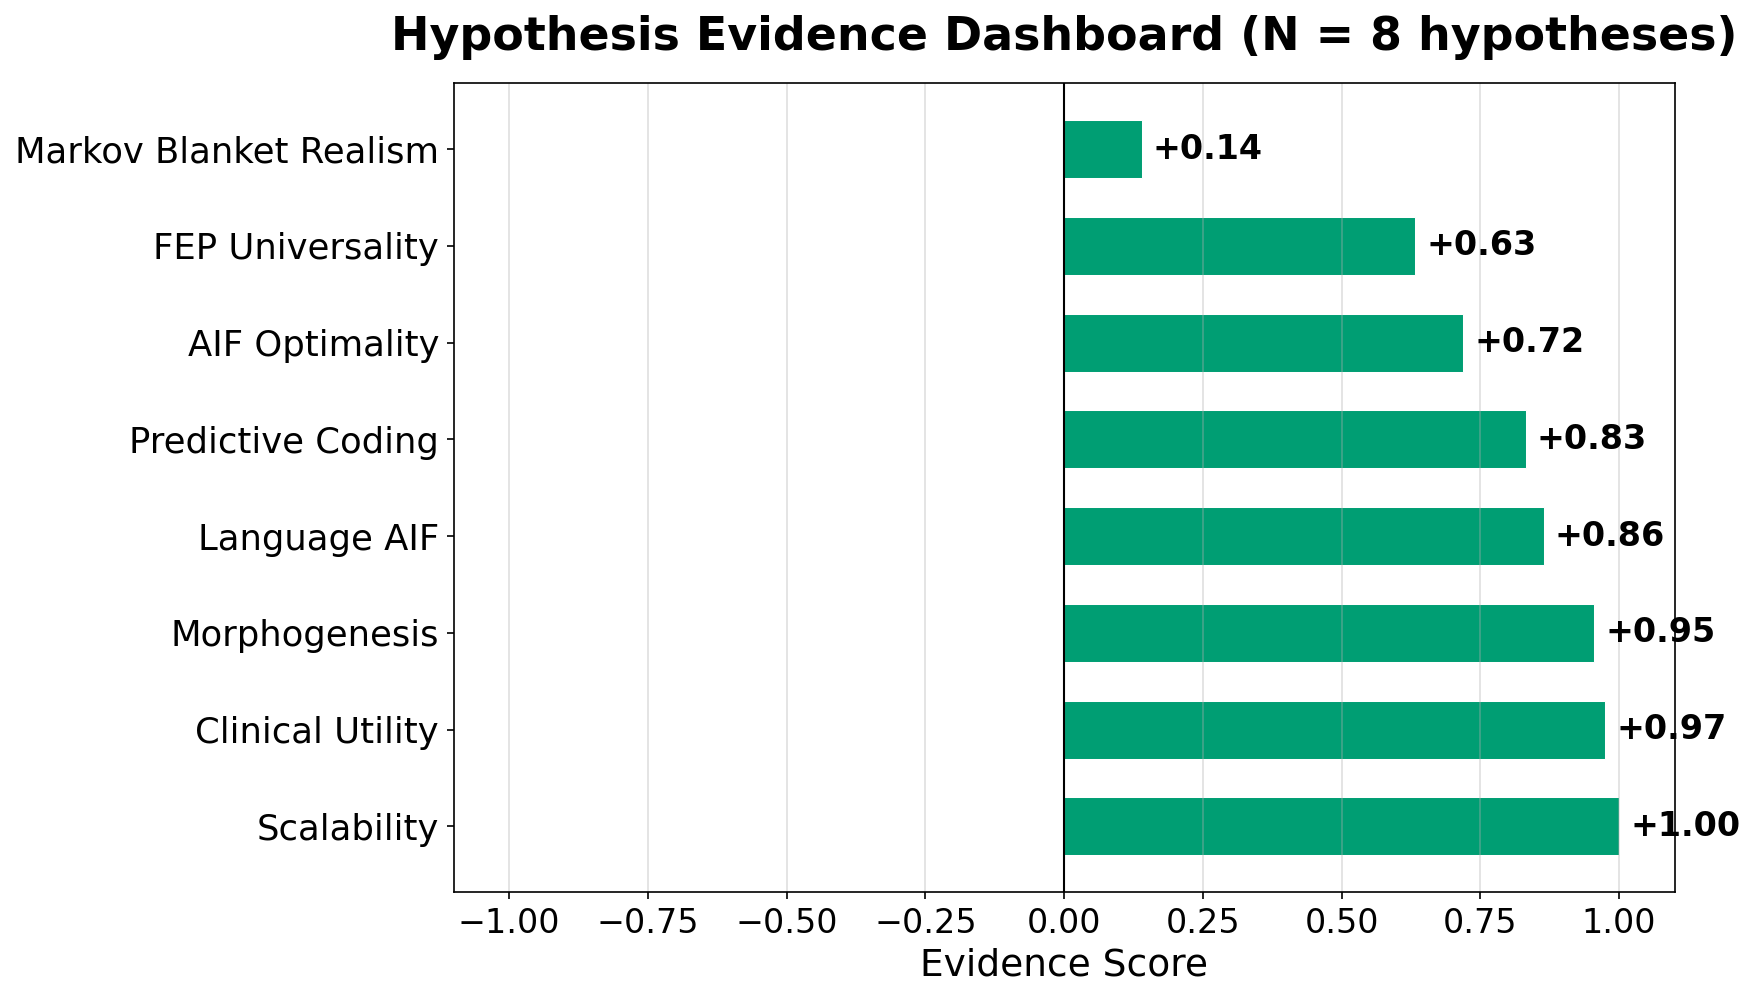
\includegraphics[width=0.9\textwidth]{../figures/hypothesis_dashboard.png}
\caption{Hypothesis scoring dashboard showing citation-weighted evidence scores ($[-1, +1]$) for the eight tracked hypotheses, sorted descending by consensus strength. Predominantly positive scores reflect both genuine empirical support and systematic positive biases from publication selection and linguistic framing (see \S\ref{sec:pub_bias}).}
\label{fig:hypothesis_dashboard}
\end{figure}

\subsubsection{Interpretation of Evidence
Profiles}\label{interpretation-of-evidence-profiles}

To directly address our core research questions---identifying which
claims are robustly supported and which remain contested---we evaluated
how the hypothesis-level evidence maps against the critiques introduced
in \S\ref{sec:methods}. The score ordering is data-derived and should be
read as a relative evidence map, not as a set of absolute
scientific-certainty tiers. The highest observed score is Scalability
(SCALABILITY) at \(+1.00\), while 8 hypotheses have positive scores and
0 have negative scores in this snapshot. FEP Universality (H1), with
1069 assertions, has the largest assessed evidence base; assertion
volume and score magnitude answer different questions. Across
hypotheses, citation-weighting captures which claims the community cites
most rather than providing a simple ballot of assertion counts; this can
amplify highly cited supportive or critical evidence. The complete score
and count table is the authoritative comparison, while the dashboard and
timeline provide visual summaries.

Markov blanket realism (H3) has 34 assertions, a score of \(+0.14\), and
14 contradicting assertions. Its relatively low positive score is
consistent with an active ontological debate between accounts that treat
Markov blankets as real thermodynamic boundaries and accounts that treat
them as instrumental statistical tools \citep{bruineberg2022emperor}; a
positive tally should not be relabeled as consensus.

FEP universality (H1) generates 1069 assertions yet achieves a score of
\(+0.63\). Neutral assessments account for 533 of those tallies,
compared with 522 supporting and 14 contradicting assertions. This
composition illustrates why a large evidence count does not imply a
strongly directional result: many papers invoke the FEP as conceptual
scaffolding without explicitly testing universality. The observation is
consistent with falsifiability critiques of broad principle-level claims
\citep{colombo2021free}, but remains an interpretation of the extracted
abstract-level evidence.

\subsubsection{Temporal Dynamics of Evidence
Accumulation}\label{temporal-dynamics-of-evidence-accumulation}

The cumulative evidence timeline (Figure \ref{fig:evidence_timeline}) is
descriptive and limited to the observed corpus years. Early years can
show extreme scores when only a small number of assertions contribute;
the updated figure reports cumulative assertion counts alongside the
score encoding. Later trajectories should be interpreted as accumulation
patterns rather than causal effects of individual papers, especially for
H5 and H6, whose evidence base is concentrated in more recent
literature. The timeline does not establish that any hypothesis became
positive before the first year represented in this corpus.

\begin{figure}[htbp]
\centering
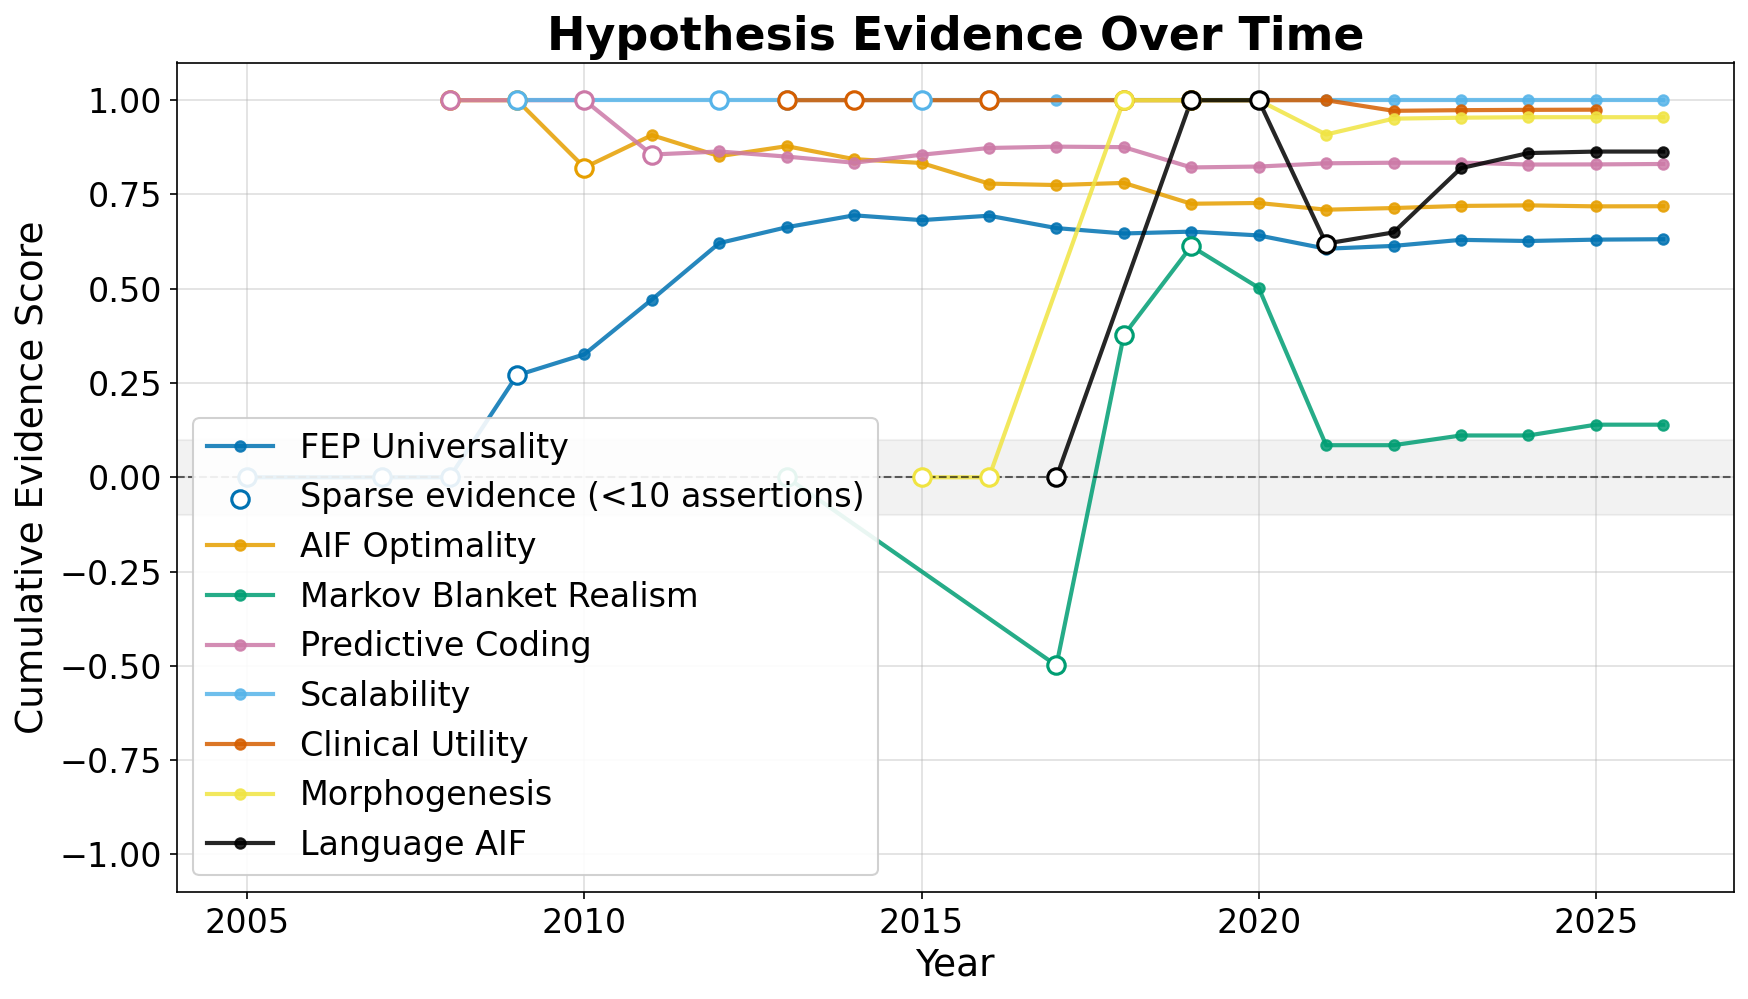
\includegraphics[width=0.9\textwidth]{../figures/evidence_timeline.png}
\caption{Temporal evolution of cumulative citation-weighted evidence scores by hypothesis (2003--2026). Marker and line encoding includes cumulative assertion counts so sparse early years are not mistaken for stable estimates.}
\label{fig:evidence_timeline}
\end{figure}

\subsubsection{Assertion Composition and
Distribution}\label{assertion-composition-and-distribution}

The per-hypothesis composition of assertions (Figure
\ref{fig:assertion_breakdown}) and the multi-panel summary (Figure
\ref{fig:assertion_summary}) provide complementary views of the
extraction results.

\begin{figure}[htbp]
\centering
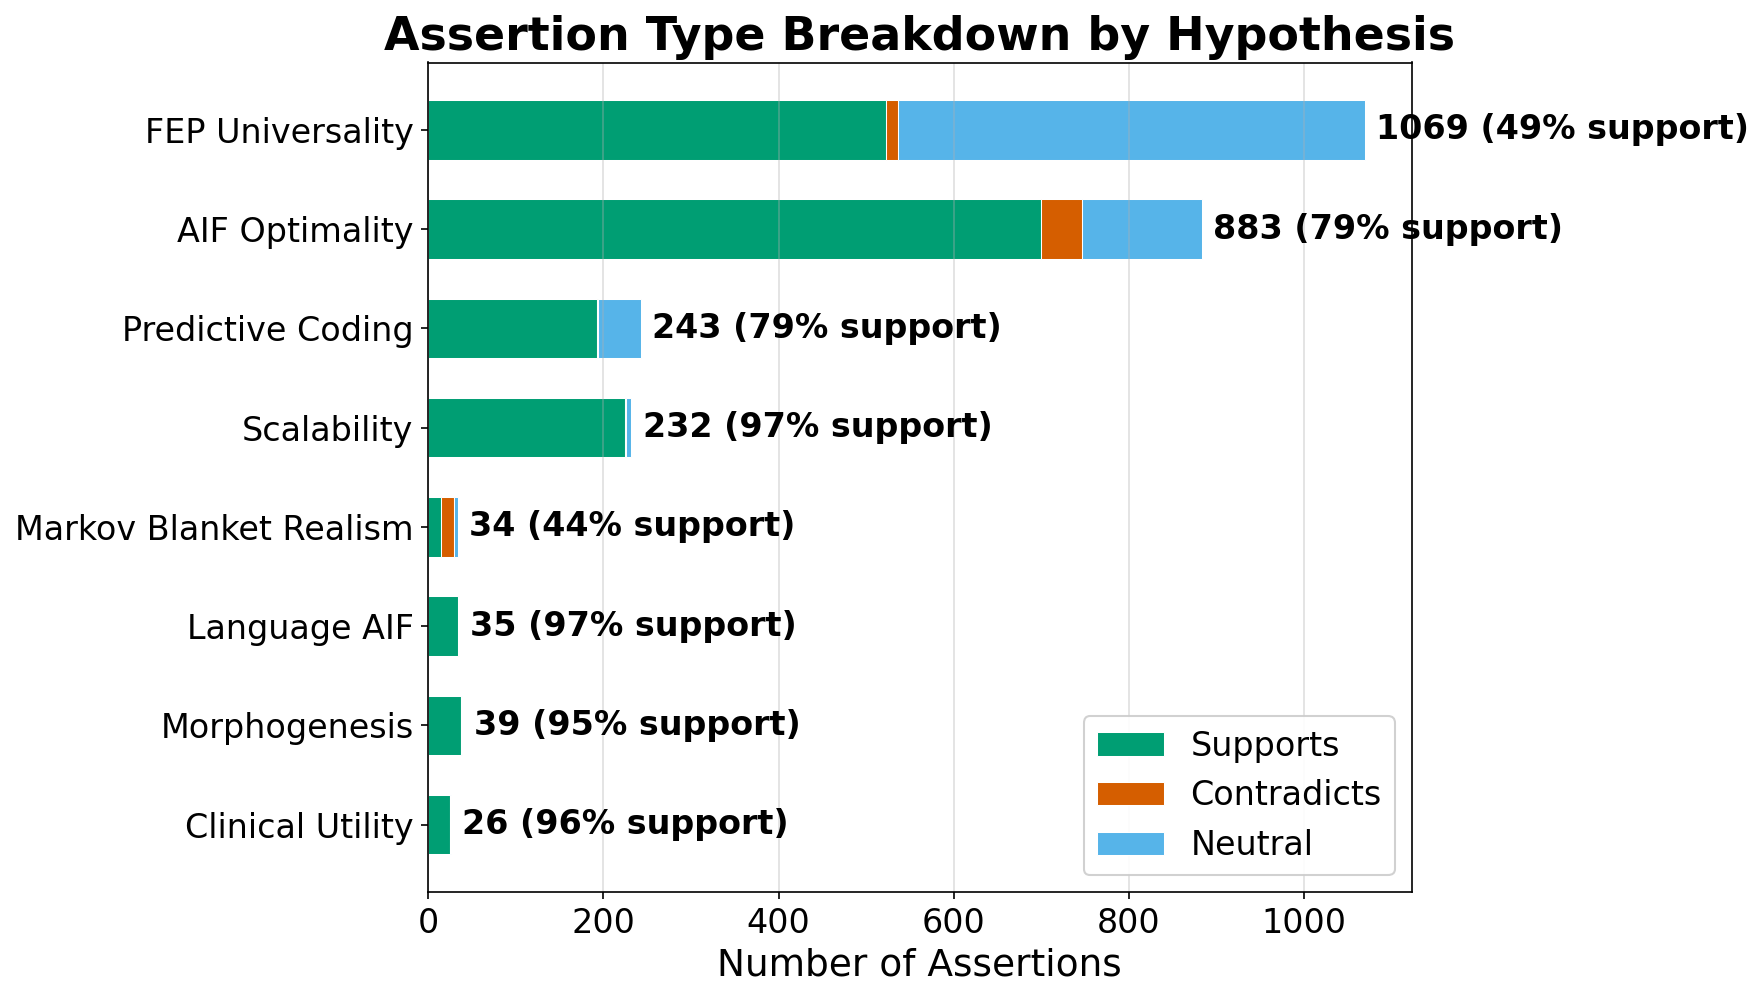
\includegraphics[width=0.9\textwidth]{../figures/assertion_breakdown.png}
\caption{Stacked horizontal bars decomposing per-hypothesis assertions into supports (green), contradicts (red-orange), and neutral (blue) categories ($N = 2,561$ total assertions). Labels show total count and support percentage. The high support fractions are partially attributable to publication bias and affirmative linguistic framing.}
\label{fig:assertion_breakdown}
\end{figure}

\begin{figure}[htbp]
\centering
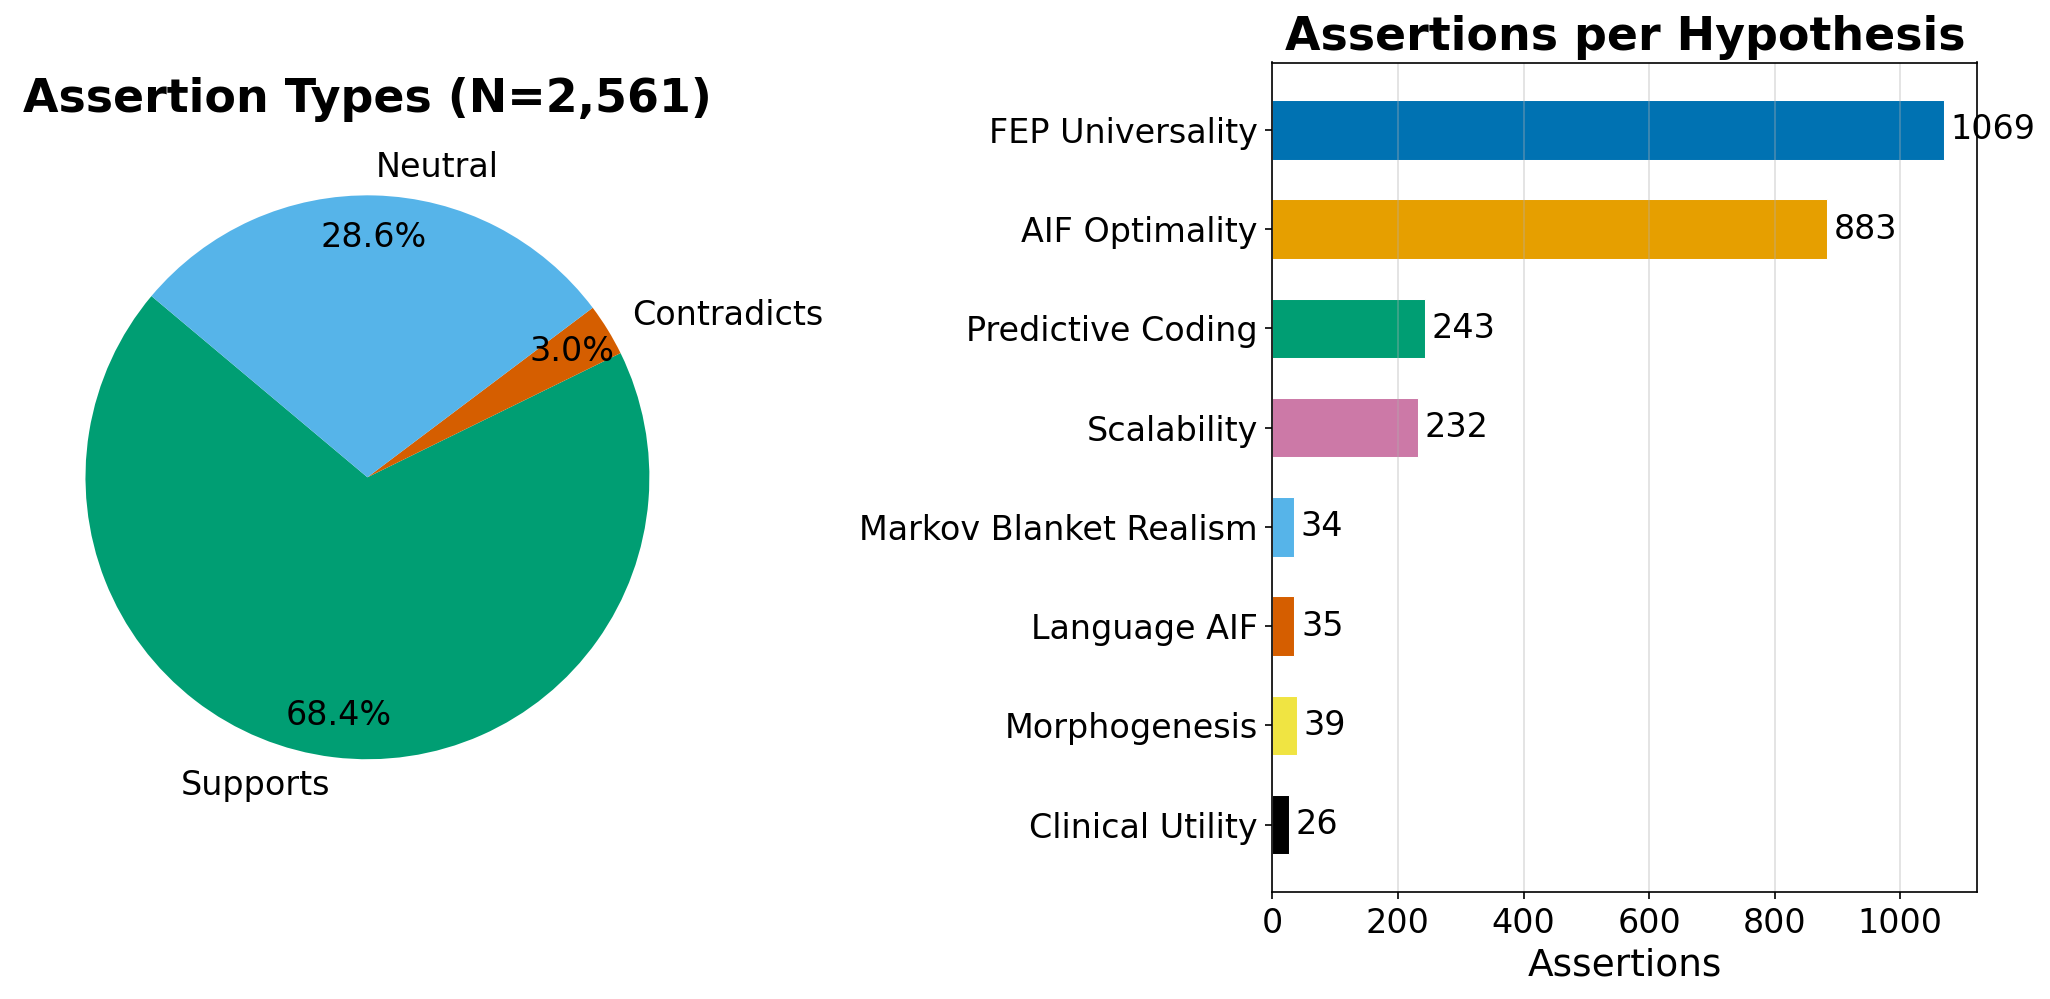
\includegraphics[width=0.9\textwidth]{../figures/assertion_summary.png}
\caption{Multi-panel assertion summary: (left) pie chart of overall assertion type distribution showing supports/contradicts/neutral proportions, (right) per-hypothesis assertion counts with palette-coded bars. $N = 2,561$ assertions extracted from $1106$ papers.}
\label{fig:assertion_summary}
\end{figure}

\subsubsection{Limitations of the Current Scoring
Approach}\label{limitations-of-the-current-scoring-approach}

\paragraph{Publication Bias and Linguistic
Asymmetry}\label{sec:pub_bias}

The mixed scores observed across the eight hypotheses should be
interpreted with two systematic caveats.

First, \textbf{publication bias} systematically inflates supporting
evidence. Academic journals preferentially publish positive and
confirmatory results (\citep{sterling1959publication}), meaning that
studies finding null or contradictory outcomes for any hypothesis are
less likely to appear in the retrievable literature. This
\textit{file-drawer effect} is well-documented across scientific
disciplines and is expected to disproportionately suppress contradicting
assertions in our extraction pipeline. The Active Inference literature
is particularly susceptible: as a theoretical framework with strong
foundational proponents, papers are more likely to frame results as
consistent with the FEP than as challenges to it.

Second, \textbf{linguistic asymmetry} in academic writing further skews
extraction toward positive classifications. Declarative scholarly claims
are inherently phrased affirmatively---authors write ``our results
support,'' ``consistent with,'' or ``extends the prediction of'' far
more frequently than ``our results refute'' or ``contradicts the claim
that.'' Because the LLM extraction pipeline operates on abstract text,
this linguistic imbalance propagates directly into the assertion
distribution. Even papers presenting genuinely mixed evidence tend to
frame their abstracts in terms of what \textit{was} found rather than
what was not, biasing the extracted direction toward ``supports.'\,'

These two effects act in concert: publication bias reduces the number of
contradicting papers in the corpus, and linguistic framing reduces the
number of contradicting assertions extracted from the papers that do
appear. Consequently, the absolute values of hypothesis scores should
not be taken as unbiased measures of scientific consensus. We retain the
relative ordering and temporal trajectories as transparent descriptive
summaries, but the present study does not establish that they are robust
to extraction error, retrieval bias, or correlated evidence.

\subsubsection{Methodological Validation and LLM
Calibration}\label{methodological-validation-and-llm-calibration}

The evidence derives from automated LLM-based assertion extraction
operating on abstracts only. A stratified rule-based reference-annotator
agreement study (\(n = 256\)) provides a first quantitative, fully
reproducible calibration: two deterministic keyword-rule protocols agree
at \(\kappa = 0.704\) (reference stability), while pipeline triage
against the primary rule reference yields precision 0.013, recall 1.000,
and F1 0.026, with reference--pipeline direction agreement of only
\(\kappa = -0.048\). That the LLM and an independent keyword reference
diverge this sharply is itself the calibration result: over-extraction
(pipeline labels relevant where the keyword reference labels irrelevant)
accounts for 0.738 of sampled rows, directly motivating the tempered
interpretation of absolute hypothesis scores. Rankings and temporal
trajectories are retained for auditability, not treated as validated
estimates. These figures are a reproducibility floor, not accuracy
against human ground truth, which remains future work. Full metrics and
error taxonomy appear in Table \ref{tab:validation_metrics}
(\S\ref{sec:extraction_pipeline}).

\subsubsection{Citation-Weighting
Sensitivity}\label{citation-weighting-sensitivity}

Hypothesis ranks under 5 alternative weight policies remain stable in
this weighting-only sensitivity check: minimum rank-stability Spearman
\(\rho = 0.976\) versus the default log-citation policy, with 2
rank-position changes across all 6 tested policies. 1 hypotheses change
sign under at least one tested policy, so sign and tier language remain
sensitivity-dependent. The largest policy shifts should be read as a
weighting diagnostic rather than as evidence of a different scientific
conclusion.

\newpage

\subsection{Field Overview: Disciplinary Structure and Growth
Dynamics}\label{sec:field_overview}

Annual output in the Active Inference literature rose from 1 papers in
2003, reaching a peak of 134 papers in 2025---a transition from a niche
within theoretical neuroscience to a multi-disciplinary research program
spanning three primary domains and eight tracked categories. The corpus
start of 2003 was chosen to capture Energy-Based Model and variational
Bayesian antecedents \citep{dayan1995helmholtz, lecun2006tutorial} that
preceded the formal introduction of the Free Energy Principle in 2006
\citep{friston2006free} and its subsequent full elaboration
\citep{friston2010free}. The configured corpus sources are arXiv,
Semantic Scholar, and OpenAlex; this snapshot records arXiv, OpenAlex
completed; Semantic Scholar incomplete and contains \(N = 1106\)
deduplicated papers (2003--2026). It therefore describes the retained
retrieval snapshot rather than an exhaustive census (Figure
\ref{fig:field_summary}).

\begin{figure}[htbp]
\centering
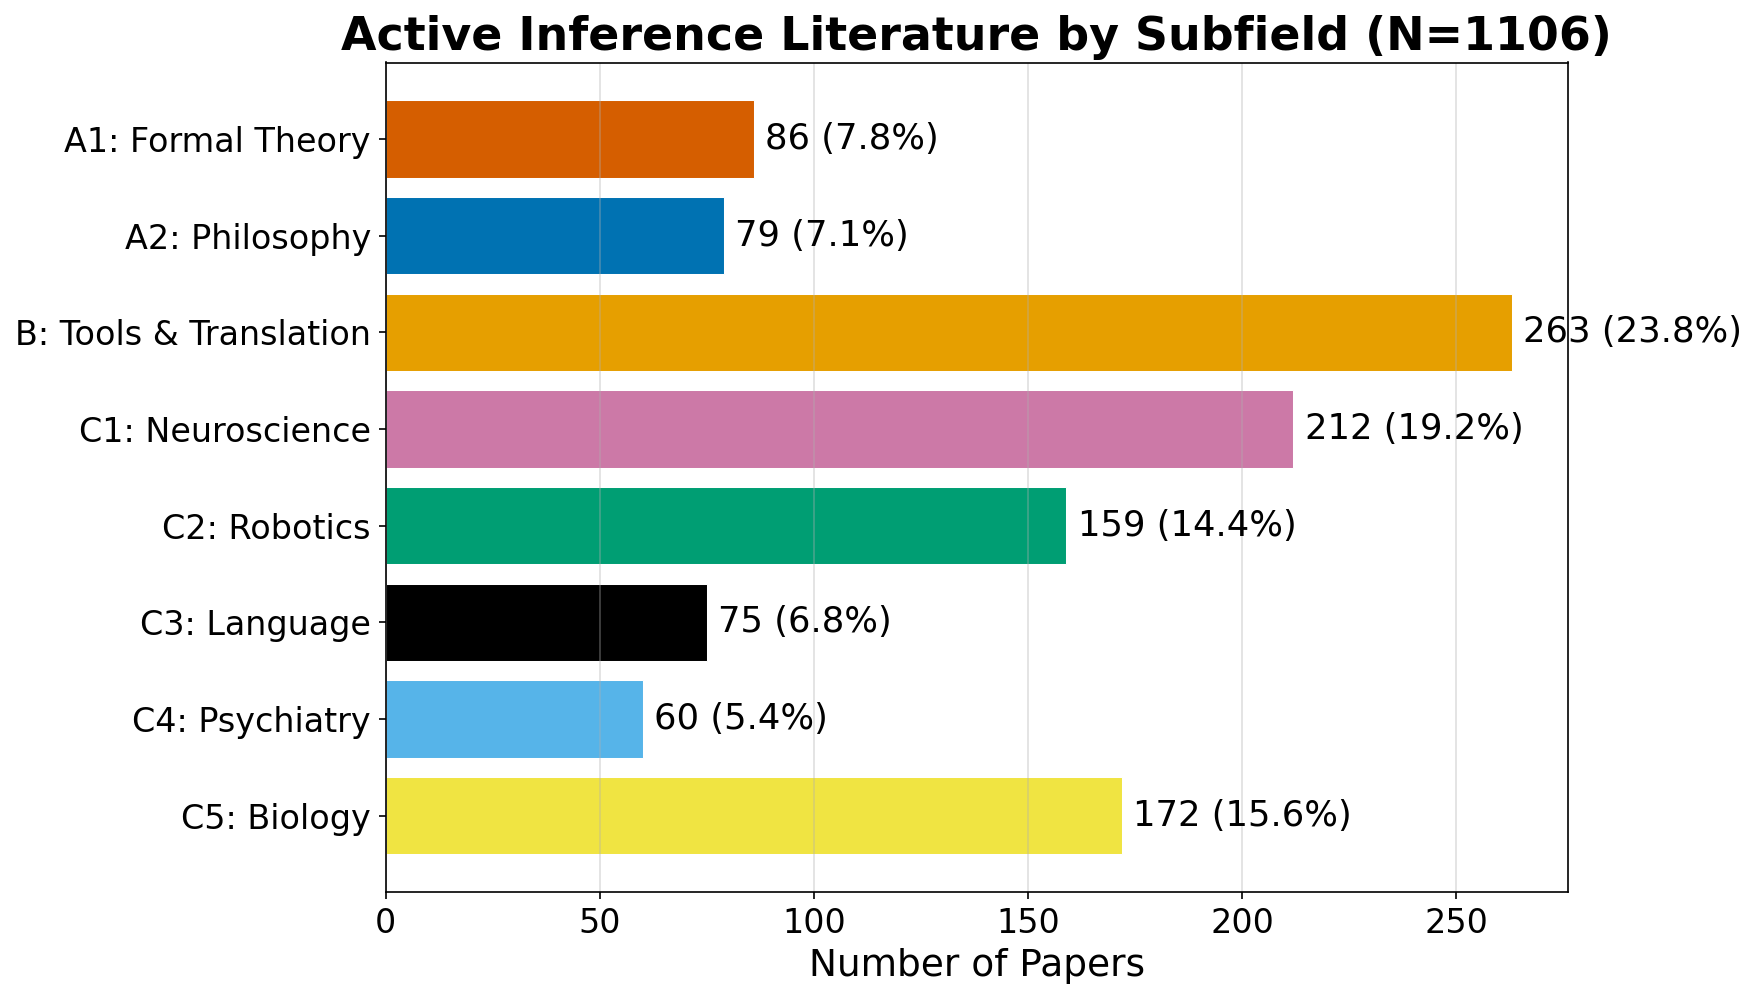
\includegraphics[width=0.9\textwidth]{../figures/field_summary.png}
\caption{Publication counts by domain ($N = 1106$). Application domains (C1--C5) collectively account for the largest share of the corpus; B tools is the largest single category in this run.}
\label{fig:field_summary}
\end{figure}

\subsubsection{Corpus-Level Summary}\label{corpus-level-summary}

\begin{table}[htbp]
\centering
\caption{Corpus-level summary statistics for the Active Inference literature corpus ($N = 1106$), observed over 2003--2026 with the most recent year reported as YTD / partial year.}
\label{tab:corpus_summary}
\begin{tabular}{ll}
\toprule
\textbf{Metric} & \textbf{Value} \\
\midrule
Total papers & 1106 \\
Year range & 2003--2026 (YTD / partial year) \\
Peak year & 2025 \\
CAGR & 24.94\% \\
Active domains & 8 of 8 tracked (A1--A2, B, C1--C5) \\
\bottomrule
\end{tabular}
\end{table}

The CAGR of 24.94\% is measured as the annualised growth rate of yearly
publication volume between complete endpoint years 2003 and 2025. The
corpus also contains 98 papers from 2026 as of 2026-07-26; this
partial-year count is shown separately in the growth figure and is not
used as the CAGR endpoint. Citation network metrics are detailed in the
dedicated citation network analysis (see
\hyperref[sec:citation_network]{the citation network analysis}).

\begin{figure}[htbp]
\centering
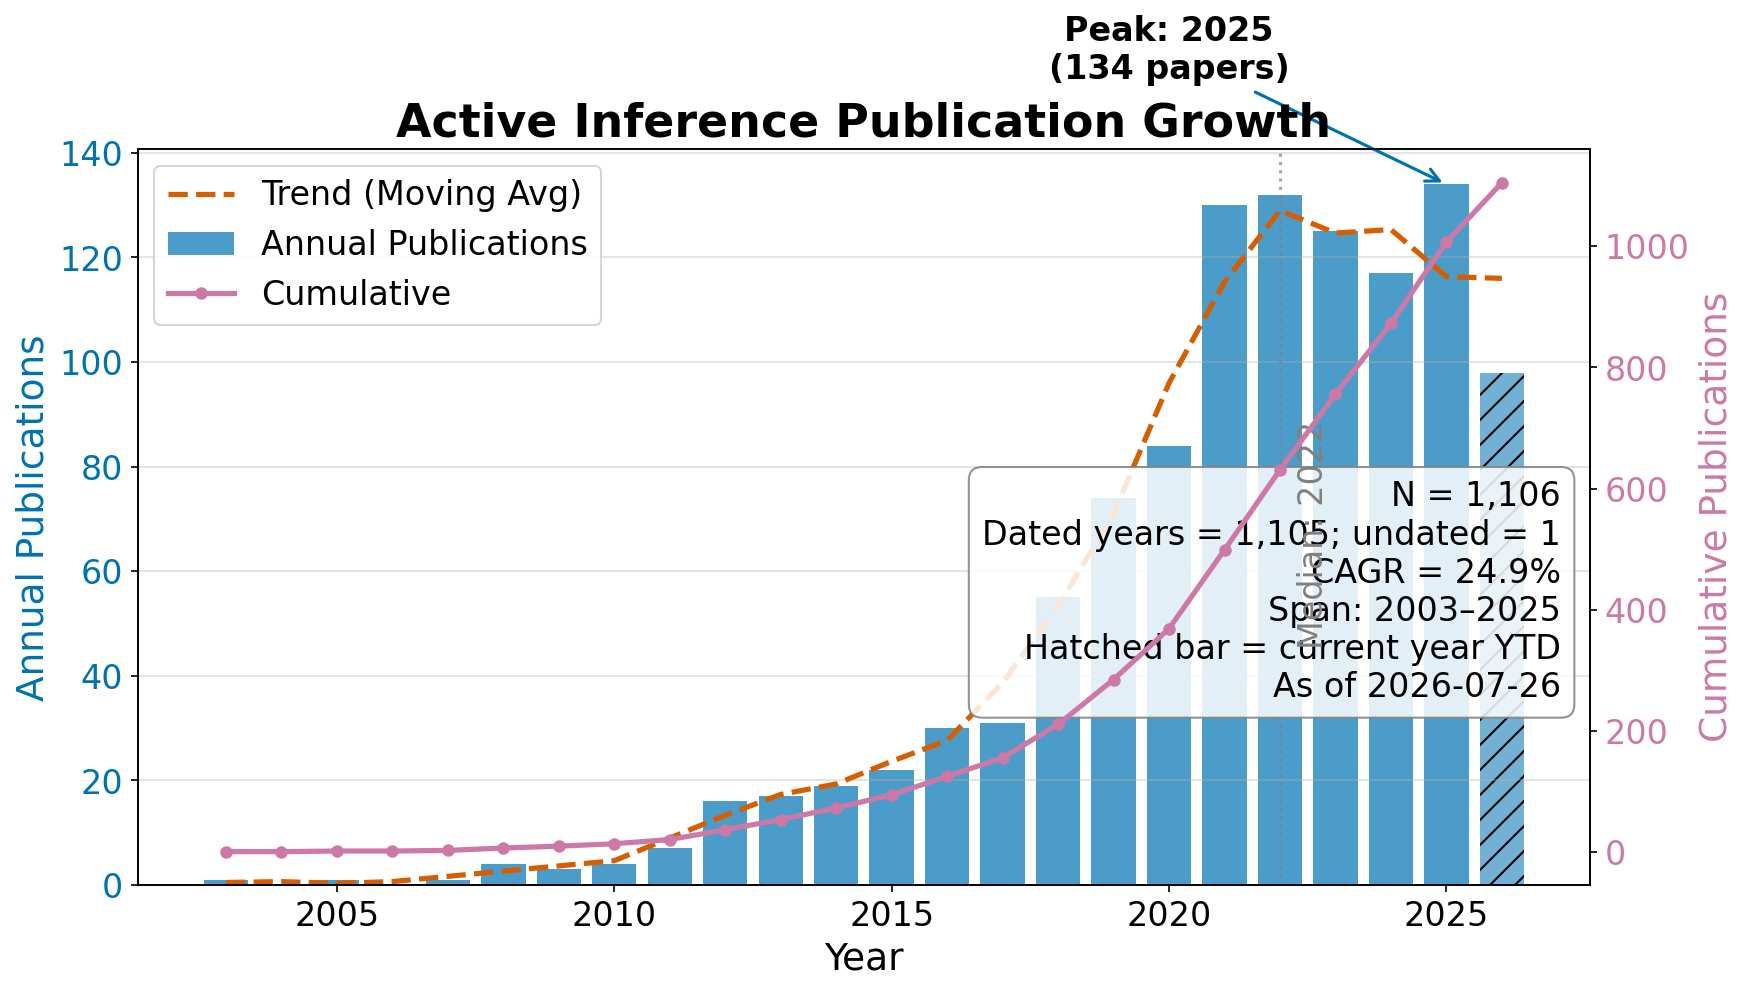
\includegraphics[width=0.8\textwidth]{../figures/growth_curve.png}
\caption{Annual (bars) and cumulative (line) publication counts, 2003--2026 ($N = 1106$, CAGR = 24.94\% over 2003–2025). The 2026 bar is partial as of 2026-07-26.}
\label{fig:growth_curve}
\end{figure}

\subsubsection{Domain Distribution}\label{domain-distribution}

Keyword-based classification assigns each paper to one of eight
categories across three domains:

\begin{table}[htbp]
\centering
\caption{Domain distribution across three tiers and eight categories ($N = 1106$ papers). Classification uses hierarchical keyword matching with priority-based routing to minimize over-assignment to catch-all categories.}
\label{tab:domain_distribution}
\begin{tabular}{llcc}
\toprule
\textbf{Domain} & \textbf{Category} & \textbf{Papers} & \textbf{Percentage} \\
\midrule
A -- Core Theory & A1: Formal Theory & 86 & 7.8\% \\
 & A2: Qualitative Philosophy & 79 & 7.1\% \\
\midrule
B -- Tools & B: Tools \& Translation & 263 & 23.8\% \\
\midrule
C -- Applications & C1: Neuroscience & 212 & 19.2\% \\
 & C2: Robotics & 159 & 14.4\% \\
 & C3: Language & 75 & 6.8\% \\
 & C4: Psychiatry & 60 & 5.4\% \\
 & C5: Biology & 172 & 15.6\% \\
\bottomrule
\end{tabular}
\end{table}

The largest single category is B tools; the counts should be read as
classifier assignments rather than as measures of disciplinary
importance (Figure \ref{fig:subfield_distribution}). The priority-based
classifier routes papers with mathematical indicators (theorems, proofs,
equations, statistical formalism) to A1 before falling back to A2, and
prefers specific application domains (C1--C5) and tools (B) over both
core-theory categories. Papers that discuss FEP/AIF conceptually without
mathematical formalism or domain-specific vocabulary are assigned to A2.
Embedding-based classification could redistribute some fraction across
categories, so the taxonomy is a reproducible map rather than a literal
measure of research focus. All eight categories are populated,
indicating diversification beyond the field's neuroscience origins.

\begin{figure}[htbp]
\centering
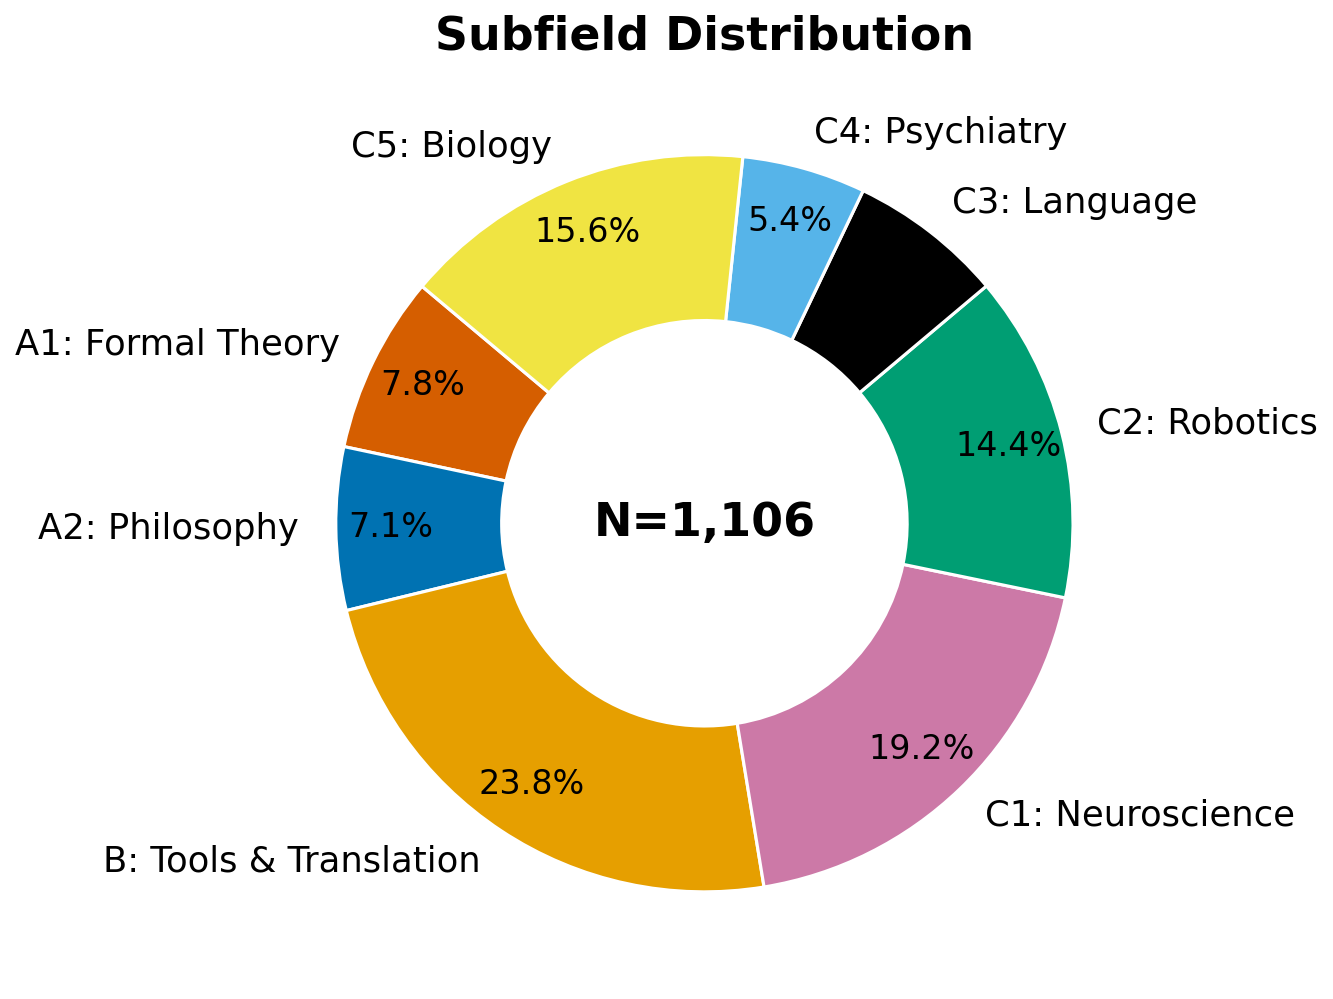
\includegraphics[width=0.8\textwidth]{../figures/subfield_distribution.png}
\caption{Domain distribution ($N = 1106$). Classification uses hierarchical keyword matching against curated lists applied to titles and abstracts, capturing distinct methodological and domain-specific groupings.}
\label{fig:subfield_distribution}
\end{figure}

Detailed characterizations of each domain---including historical
context, growth trends, and open problems---are provided in the
supplementary domain analyses (see
\hyperref[sec:subfield_analyses]{the domain analyses}). Latent topic
structure, vocabulary analysis, and document embeddings are presented in
the text analytics section (see
\hyperref[sec:text_analytics]{the text analytics section}).

\subsubsection{Cross-Domain Comparison}\label{cross-domain-comparison}

\begin{table}[htbp]
\centering
\caption{Cross-domain comparison showing growth trajectories, maturity levels, key challenges, and representative publications for each of the eight tracked categories. Growth trends and maturity assessments are based on temporal publication patterns and evidence base depth.}
\label{tab:cross_domain_comparison}
\begin{tabular}{llcllll}
\toprule
\textbf{Domain} & \textbf{Category} & \textbf{Papers} & \textbf{Growth} & \textbf{Maturity} & \textbf{Key Challenge} & \textbf{Rep.\ Work} \\
\midrule
A & A1: Formal & 86 (7.8\%) & Growing & Mature & Math accessibility & \citep{sakthivadivel2023bayesian} \\
A & A2: Philosophy & 79 (7.1\%) & Stable & Mature & Catch-all absorption & \citep{friston2010free} \\
B & B: Tools & 263 (23.8\%) & Rapid & Growing & Deep RL benchmarks & \citep{fountas2020deep} \\
C & C1: Neuroscience & 212 (19.2\%) & Stable & Mature & Theory--neuroimaging gap & \citep{clark2013whatever} \\
C & C2: Robotics & 159 (14.4\%) & Growing & Growing & Embedded real-time & \citep{lanillos2021active} \\
C & C3: Language & 75 (6.8\%) & Emerging & Nascent & NLP model comparison & \citep{friston2020generative} \\
C & C4: Psychiatry & 60 (5.4\%) & Emerging & Nascent & Clinical translation & \citep{smith2021computational} \\
C & C5: Biology & 172 (15.6\%) & Rapid & Nascent & Empirical validation & \citep{kuchling2020morphogenesis} \\
\bottomrule
\end{tabular}
\end{table}

Three structural features emerge from the cross-domain comparison
(Figure \ref{fig:subfield_timeline}). Ranked by corpus share, the
domains are Domain C (Applications) (61.3\%), Domain B (Tools and
Translation) (23.8\%), Domain A (Core Theory) (14.9\%). Domain C is
therefore the largest descriptive tier in this snapshot, while Domain
A's smaller share does not measure its intellectual influence: the
mathematical formalisms developed in A1 shape implementations across all
domains. The emergent application frontiers (C3--C5) should be
interpreted through their temporal trajectories rather than assumed to
be uniformly accelerating.

\begin{figure}[htbp]
\centering
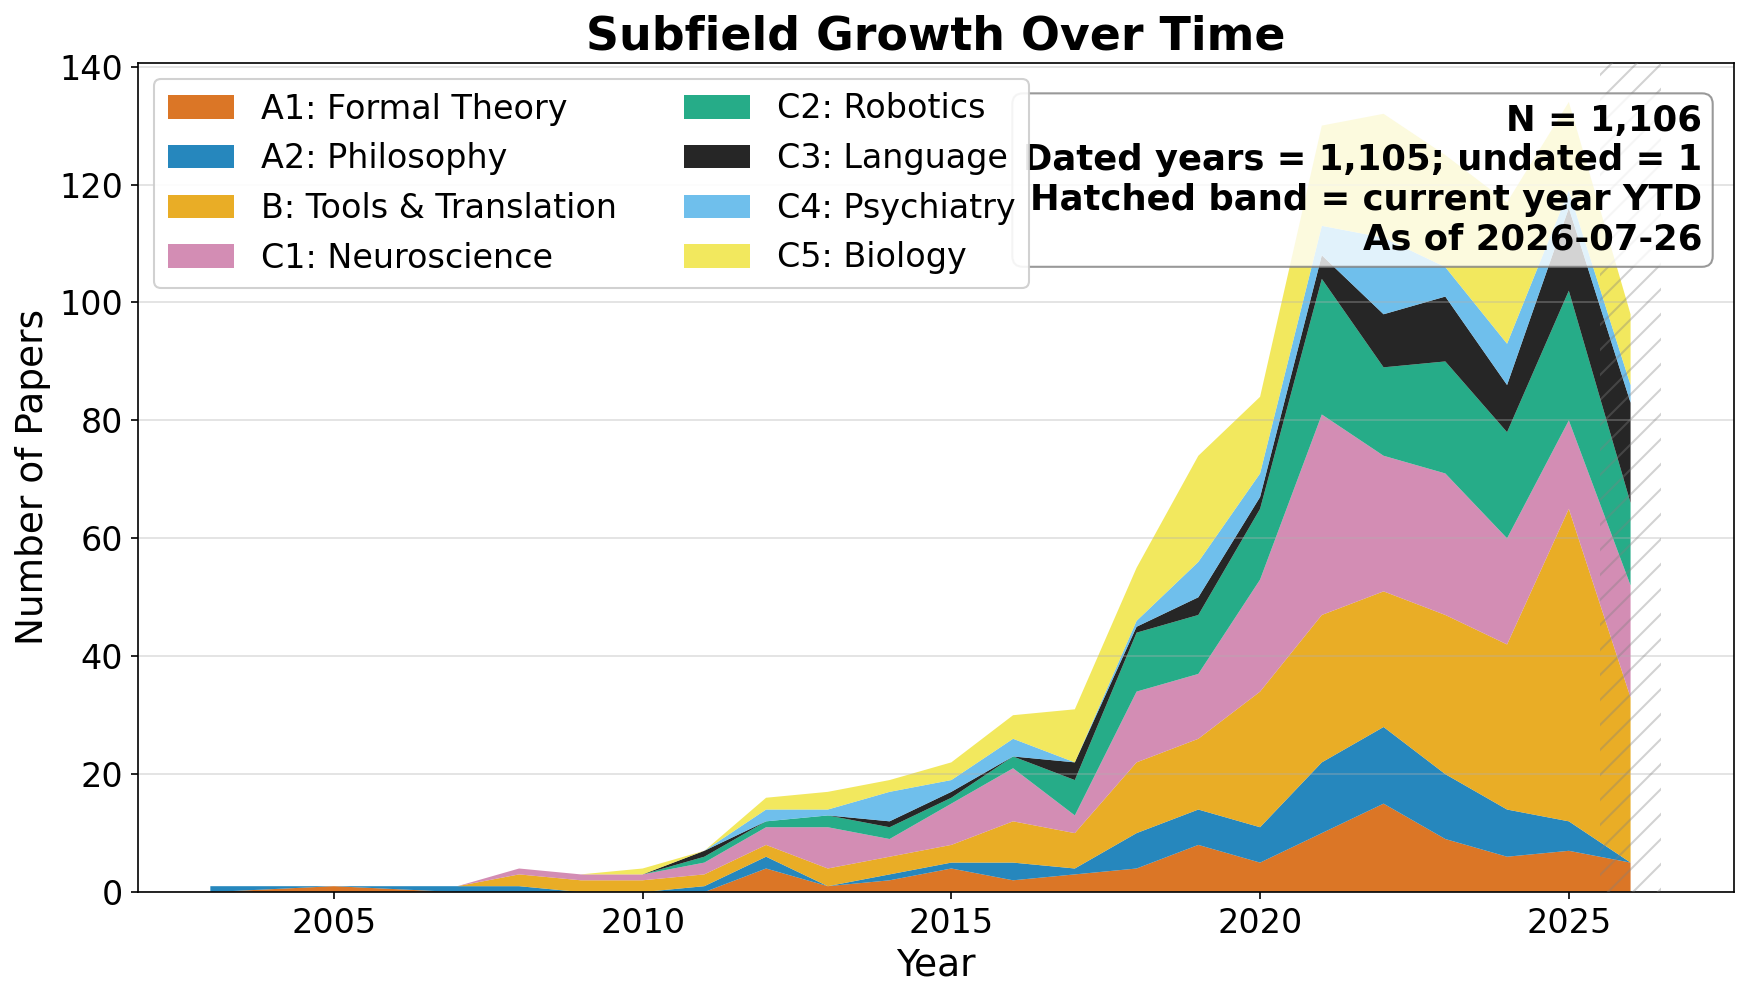
\includegraphics[width=0.9\textwidth]{../figures/subfield_timeline.png}
\caption{Stacked area chart of publications by domain, 2003--2026 ($N = 1106$). The current-year observation is partial as of 2026-07-26; the chart reports classifier-assigned category totals and temporal composition.}
\label{fig:subfield_timeline}
\end{figure}

\newpage

\subsection{Domain Analyses: Growth Trajectories and Open
Problems}\label{sec:subfield_analyses}

\emph{This supplementary section provides detailed characterizations of
each of the eight tracked Active Inference domains, organized under
three tiers: A (Core Theory), B (Tools \& Translation), and C
(Application Domains).}

\subsubsection{Domain A: Core Theory}\label{domain-a-core-theory}

\paragraph{A1 --- Quantitative and Formal Theory (n = 86, 7.8
percent)}\label{a1-quantitative-and-formal-theory-n-86-7.8-percent}

The A1 domain develops the mathematical foundations underpinning the
Free Energy Principle: information geometry, category-theoretic
formulations of Markov blankets, path integral formulations of free
energy minimization, and gauge-theoretic perspectives on
self-organization. A central debate concerns the ontological status of
Markov blankets---whether they correspond to real physical boundaries or
are merely useful statistical constructs \citep{bruineberg2022emperor}.
Bruineberg et al.~draw a critical distinction between \emph{Pearl
blankets} (instrumental, epistemic tools for conditional independence in
Bayesian networks) and \emph{Friston blankets} (ontologically laden
physical boundaries between agent and environment), arguing that the
scientific credibility of the former should not be extended uncritically
to the latter. Friston and collaborators continue to address this
critique through the development of Bayesian mechanics
\citep{sakthivadivel2023bayesian}, which aims to place the FEP on firmer
mathematical footing by grounding Markov blanket dynamics in the physics
of belief-based systems. Our hypothesis scoring quantifies this debate:
the Markov blanket realism hypothesis (H3) achieves a score of \(+0.14\)
with 14 contradicting assertions, indicating a contested evidence
profile rather than resolving the ontological question. Recent
theoretical consolidation has strengthened the formal tools available to
A1: variational message passing formulations
\citep{champion2021realizing} connect expected free energy
decomposition---into risk, ambiguity, epistemic, and instrumental
components---to practical planning algorithms, advancing the theoretical
justification for EFE-based policy selection. Path integral formulations
now connect Markov blanket dynamics to least-action principles, framing
free energy minimization as paths of least action for belief updating.
With 86 papers (7.8\% of the corpus), A1 captures a meaningful share of
formal work, reflecting the improved classifier's ability to route
papers with mathematical formalism (theorems, proofs, convergence,
posterior distributions, Fokker--Planck equations) into this domain
rather than the qualitative philosophy catch-all. \textbf{Key evidence
gap:} A mathematically formal distinction yielding testable predictions
that differentiate systems actively minimizing an internal free energy
functional from systems that merely possess a Markov blanket.

\paragraph{A2 --- Qualitative Philosophy and General Theory (n = 79, 7.1
percent)}\label{a2-qualitative-philosophy-and-general-theory-n-79-7.1-percent}

The A2 domain encompasses papers that develop, extend, or review the
core Free Energy Principle and Active Inference framework without
restricting attention to a specific application domain. This includes
Friston's foundational work on variational free energy minimization
\citep{friston2010free}, the textbook treatment by Parr, Pezzulo, and
Friston \citep{parr2022active}, and numerous tutorial and review papers.
The priority-based classifier mitigates over-assignment to A2 by routing
papers with mathematical formalism to A1 and papers with domain-specific
vocabulary to C1--C5 or B before the A2 catch-all is reached.
Nevertheless, the count likely still conceals meaningful internal
structure: papers addressing embodied cognition, Bayesian brain theory,
and philosophical implications of the FEP are all subsumed under this
heading.

Three unresolved debates drive the most contested A2 literature. First,
the \textbf{explanatory scope} question: is the FEP a principle of
physics (applying to any system at non-equilibrium steady state
\citep{friston2010free}), a principle of biology (restricted to
organisms that actively maintain their boundaries against entropy), or a
computational-level description of cognition \citep{clark2013whatever}?
The answer determines whether evidence from robotics, synthetic biology,
or cellular dynamics counts as genuine support for the FEP or merely
analogical illustration. Second, the \textbf{relationship to
reinforcement learning}: active inference and deep RL both minimize
expected future cost, but differ in whether the objective is expected
free energy (AIF) or expected cumulative reward (RL). Establishing
formal equivalence or principled divergence between these frameworks is
prerequisite for the benchmark comparisons domain B requires. Third,
\textbf{eliminativist vs.~instrumentalist interpretations} of free
energy itself---whether variational free energy is a latent quantity the
brain actually tracks or a mathematical convenience for describing
inference---remain open, with consequences for the empirical status of
A1 formalisms. \textbf{Key evidence gap:} A head-to-head theoretical
comparison showing conditions under which active inference makes
predictions that differ from reinforcement learning, optimal control, or
Bayesian brain models, together with experimental designs capable of
adjudicating among them.

\subsubsection{Domain B: Tools and Translation
Methods}\label{domain-b-tools-and-translation-methods}

\paragraph{B --- Algorithms, Scaling, and Software (n = 263, 23.8
percent)}\label{b-algorithms-scaling-and-software-n-263-23.8-percent}

Domain B addresses the computational challenge of making active
inference practical in complex, high-dimensional environments. Early
implementations relied on small discrete state spaces amenable to exact
message passing. Recent work has introduced deep active inference using
neural networks to amortize inference \citep{fountas2020deep}, Monte
Carlo tree search for planning \citep{champion2021realizing}, hybrid
architectures combining model-based planning with model-free components,
and interpretable alternatives such as Free Energy Projective Simulation
(FEPS) \citep{pazem2024feps}, which exposes decision logic as
human-readable policy graphs. The central open question is whether
active inference agents can match deep reinforcement learning
performance on standard benchmarks while retaining interpretability and
sample efficiency. The availability of the pymdp library
\citep{heins2022pymdp} has lowered implementation barriers, contributing
to this domain's growth. The recent establishment of the Pymdp
Fellowship program (funding 8 open-source developers in 2025) and the
release of real-time stream processing tools like RxInfer.jl v4.0.0
\citep{rxinfer2025} indicate a vibrant and maturing software ecosystem.
\textbf{Key evidence gap:} Head-to-head benchmarking of AIF agents
against state-of-the-art deep RL baselines on standardized,
continuous-control or long-horizon environments.

\subsubsection{Domain C: Application
Domains}\label{domain-c-application-domains}

\paragraph{C1 --- Neuroscience (n = 212, 19.2
percent)}\label{c1-neuroscience-n-212-19.2-percent}

Neuroscience represents the historical core of the Active Inference
research program. The predictive processing account---in which cortical
hierarchies minimize prediction errors through both perceptual inference
and active sampling---remains one of the most empirically tested aspects
of the framework \citep{friston2010free, clark2013whatever}. The broader
neuroscience literature on Dynamic Causal Modeling and predictive coding
is extensive; the relatively modest count here likely reflects the
keyword classifier's inability to distinguish neuroscience-specific
applications from general FEP theory. Bridging the gap between
computational models and empirical neuroimaging data remains the
domain's primary challenge.

\paragraph{C2 --- Robotics (n = 159, 14.4
percent)}\label{c2-robotics-n-159-14.4-percent}

Robotics applications treat embodied agents as free energy minimizing
systems that unify perception and action through proprioceptive and
exteroceptive prediction errors \citep{lanillos2021active}. Applications
include robotic arm control, mobile navigation, manipulation, and
multi-robot coordination. Active inference offers roboticists a
principled framework for integrating sensory processing, motor planning,
and adaptive behavior without separate perception and control modules.
Key challenges include real-time computational feasibility on embedded
hardware, continuous high-dimensional action spaces, and sim-to-real
transfer.

\paragraph{C3 --- Language Processing (n = 75, 6.8
percent)}\label{c3-language-processing-n-75-6.8-percent}

The C3 domain conceptualizes linguistic processes---speech perception,
sentence comprehension, dialogue, and reading---as active inference
operating over deep hierarchical generative models of linguistic
structure \citep{friston2020generative}. Active inference models of
reading have reproduced saccadic eye-movement patterns, while models of
speech perception capture how listeners integrate prior expectations
with acoustic evidence. Recent work couples active inference to large
language models, pragmatics, and multi-agent communication. The
connection between AIF and LLMs runs in both directions: Wen
\citep{wen2025missing} proposes that AIF can replace external reward
signals in LLM-based agents, while Friston et
al.~\citep{friston2025active} demonstrate how active inference enables
artificial reasoning through structure learning via Bayesian Model
Reduction. The language domain is also where AIF shows strong results
through novel discrete generative models for structured sequential tasks
\citep{millidge2024retrospective}.

\paragraph{C4 --- Computational Psychiatry (n = 60, 5.4
percent)}\label{c4-computational-psychiatry-n-60-5.4-percent}

Computational psychiatry leverages active inference to model psychiatric
conditions as disruptions in belief updating, precision weighting, or
prior rigidity \citep{smith2021computational}. Schizophrenia has been
modeled as impaired precision weighting on bottom-up prediction errors;
depression as over-precise negative priors; and autism spectrum
conditions as atypical precision allocation over sensory channels.
Beyond clinical psychopathology, the framework is now being extended to
model higher-order cognition: Whyte et
al.~\citep{whyte2025metacognitive} propose a metacognitive active
inference account of imaginative experience, in which ``inner screen''
representations emerge from EFE-driven attention allocation under FEP
constraints---connecting computational psychiatry to consciousness
research. The domain continues to expand, with emerging frameworks
integrating psychodynamic theory (e.g., self-identity formation via
embodied interactions) with predictive processing to unify environmental
and biological factors underlying stress disorders. Translating these
computational models into diagnostic markers and therapeutic protocols
remains an ongoing challenge. \textbf{Key evidence gap:} Translating
retrodictive computational phenotyping models into prospective clinical
predictions that demonstrably outperform standard diagnostic criteria in
clinical trials.

\paragraph{C5 --- Biology and Morphogenesis (n = 172, 15.6
percent)}\label{c5-biology-and-morphogenesis-n-172-15.6-percent}

The C5 domain applies active inference and the FEP to biological systems
beyond the brain: cellular behavior, morphogenesis, evolutionary
dynamics, and the origins of life. Morphogenetic processes have been
modeled as collective active inference, where groups of cells coordinate
to minimize a shared free energy functional
\citep{kuchling2020morphogenesis, levin2022technological}. Recent
empirical work has validated collective AIF at larger scales: Heins et
al.~\citep{heins2024collective} demonstrated that surprise minimization
alone produces realistic collective motion patterns, providing a
principled alternative to ad hoc flocking rules. The FEP's reach now
extends beyond biological organisms into engineered systems: Nazemi et
al.~\citep{nazemi2025energy} apply active inference to smart building
energy control under partial observability and privacy constraints,
demonstrating that the free energy framework can govern resource
allocation in cyber-physical systems. With 172 papers, C5 reflects
growing interest in extending the FEP to encompass all self-organizing
systems---living and artificial---though the ratio of theoretical
proposals to empirical validation remains high.

\subsubsection{Comparative Synthesis}\label{comparative-synthesis}

Taken together, the three domains reveal a field transitioning from a
focused neuroscience program to a broad interdisciplinary framework.
Domain C is the largest descriptive tier in this snapshot, Domain B
pursues engineering viability through scalable algorithms and software,
and Domain A provides the theoretical and mathematical substrate. Domain
C tests the framework's generality across neuroscience (C1), robotics
(C2), language (C3), psychiatry (C4), and biology (C5). The consistent
pattern across applied domains---strong theoretical motivation paired
with limited empirical validation---suggests that the field's next
growth phase will depend on accumulating experimental evidence.

In direct response to \textbf{RQ1} (How is the Active Inference field
structured?), the domain taxonomy reveals an asymmetric three-tier
architecture: a large application tier (C), a translational layer (B),
and a smaller theoretical tier (A) in the retrieved corpus. The keyword
classifier can still mask internal diversity within each tier, so the
architecture is a reproducible classification map rather than a claim
about scientific importance.

\paragraph{Domain--Hypothesis
Cross-Reference}\label{domainhypothesis-cross-reference}

Each domain has a primary hypothesis linkage (see the detailed
hypothesis evidence analysis in the
\hyperref[sec:hypothesis_results]{hypothesis results}):

\begin{table}[htbp]
\centering
\caption{Domain--hypothesis cross-reference linking each of the eight tracked categories to its primary hypothesis and the direction of the current evidence base. Quantitative scores and temporal trends are reported in the hypothesis results section.}
\label{tab:domain_hypothesis_crossref}
\begin{tabular}{llcll}
\toprule
\textbf{Domain} & \textbf{Category} & $n$ & \textbf{Primary Hypothesis} & \textbf{Evidence Direction} \\
\midrule
A1 & Formal & 86 & H3 Markov Blanket Realism & Contested \\
A2 & Philosophy & 79 & H1 FEP Universality & Strongly supporting \\
B & Tools & 263 & H5 Scalability & Mixed \\
C1 & Neuroscience & 212 & H4 Predictive Coding & Supporting \\
C2 & Robotics & 159 & H2 AIF Optimality, H5 Scalability & Mixed \\
C3 & Language & 75 & H8 Language AIF & Emerging \\
C4 & Psychiatry & 60 & H6 Clinical Utility & Supporting \\
C5 & Biology & 172 & H7 Morphogenesis & Supporting \\
\bottomrule
\end{tabular}
\end{table}

The evidence directions summarized above are elaborated
quantitatively---with citation-weighted scores, temporal trends, and
three-tier evidence profiling---in the
\hyperref[sec:hypothesis_results]{hypothesis results section}.

\newpage

\subsubsection{Text Analytics: Topic Modeling, Vocabulary Structure, and
Document Embeddings}\label{sec:text_analytics}

This section examines the latent semantic structure of the Active
Inference corpus through complementary text-analytic methods:
non-negative matrix factorization for topic discovery, TF-IDF vocabulary
analysis, document embedding projections, and term co-occurrence
patterns. Together, these analyses reveal thematic structure that cuts
across the keyword-based domain taxonomy presented in the
\hyperref[sec:field_overview]{field overview}.

\subsubsection{Topic Modeling: Latent
Structure}\label{topic-modeling-latent-structure}

Non-negative matrix factorization (NMF) applied to the TF-IDF matrix
identifies 8 latent topics:

\begin{table}[htbp]
\centering
\caption{Non-negative matrix factorization (NMF) topic decomposition of the corpus TF-IDF matrix ($k = 8$ topics). Top terms are ranked by NMF component weight; interpretations reflect dominant thematic content.}
\label{tab:nmf_topics}
\begin{tabular}{clp{6cm}}
\toprule
\textbf{Topic} & \textbf{Top Terms} & \textbf{Interpretation} \\
\midrule
0 & cognitive, ai, social, human, cognition, systems, self, framework, consciousness, embodied & Dominant terms: cognitive, ai, social, human, cognition, systems, self, framework, consciousness, embodied \\
1 & neural, networks, network, quantum, neuronal, variational, local, dynamics, learning, activity & Dominant terms: neural, networks, network, quantum, neuronal, variational, local, dynamics, learning, activity \\
2 & fep, principle, systems, brain, free, theoretical, energy, theory, principles, argue & Dominant terms: fep, principle, systems, brain, free, theoretical, energy, theory, principles, argue \\
3 & energy, free, principle, variational, states, systems, bayesian, expected, information, markov & Dominant terms: energy, free, principle, variational, states, systems, bayesian, expected, information, markov \\
4 & inference, active, control, optimal, theory, framework, bayesian, problem, planning, decision & Dominant terms: inference, active, control, optimal, theory, framework, bayesian, problem, planning, decision \\
5 & data, models, learning, training, model, algorithm, generative, based, divergence, sampling & Dominant terms: data, models, learning, training, model, algorithm, generative, based, divergence, sampling \\
6 & sensory, predictive, brain, perception, precision, prediction, action, model, body, visual & Dominant terms: sensory, predictive, brain, perception, precision, prediction, action, model, body, visual \\
7 & agent, agents, aif, environments, learning, exploration, model, environment, reward, behavior & Dominant terms: agent, agents, aif, environments, learning, exploration, model, environment, reward, behavior \\
\bottomrule
\end{tabular}
\end{table}

\paragraph{Topic--Domain Overlap}\label{topicdomain-overlap}

The topic descriptors are partially orthogonal to the domain taxonomy,
providing an exploratory view of cross-cutting vocabulary rather than a
replacement for the supervised keyword categories. Across the configured
alternate random seeds, the mean top-term-set Jaccard similarity is
0.545 (minimum 0.407). This is a stability diagnostic for the
exploratory decomposition, not evidence that the topics are globally
unique or optimal. The absence of retrieval noise should likewise be
interpreted as a property of this query and corpus, not as a proof of
exhaustive relevance filtering (Figure \ref{fig:topic_term_bars}).

\begin{figure}[htbp]
\centering
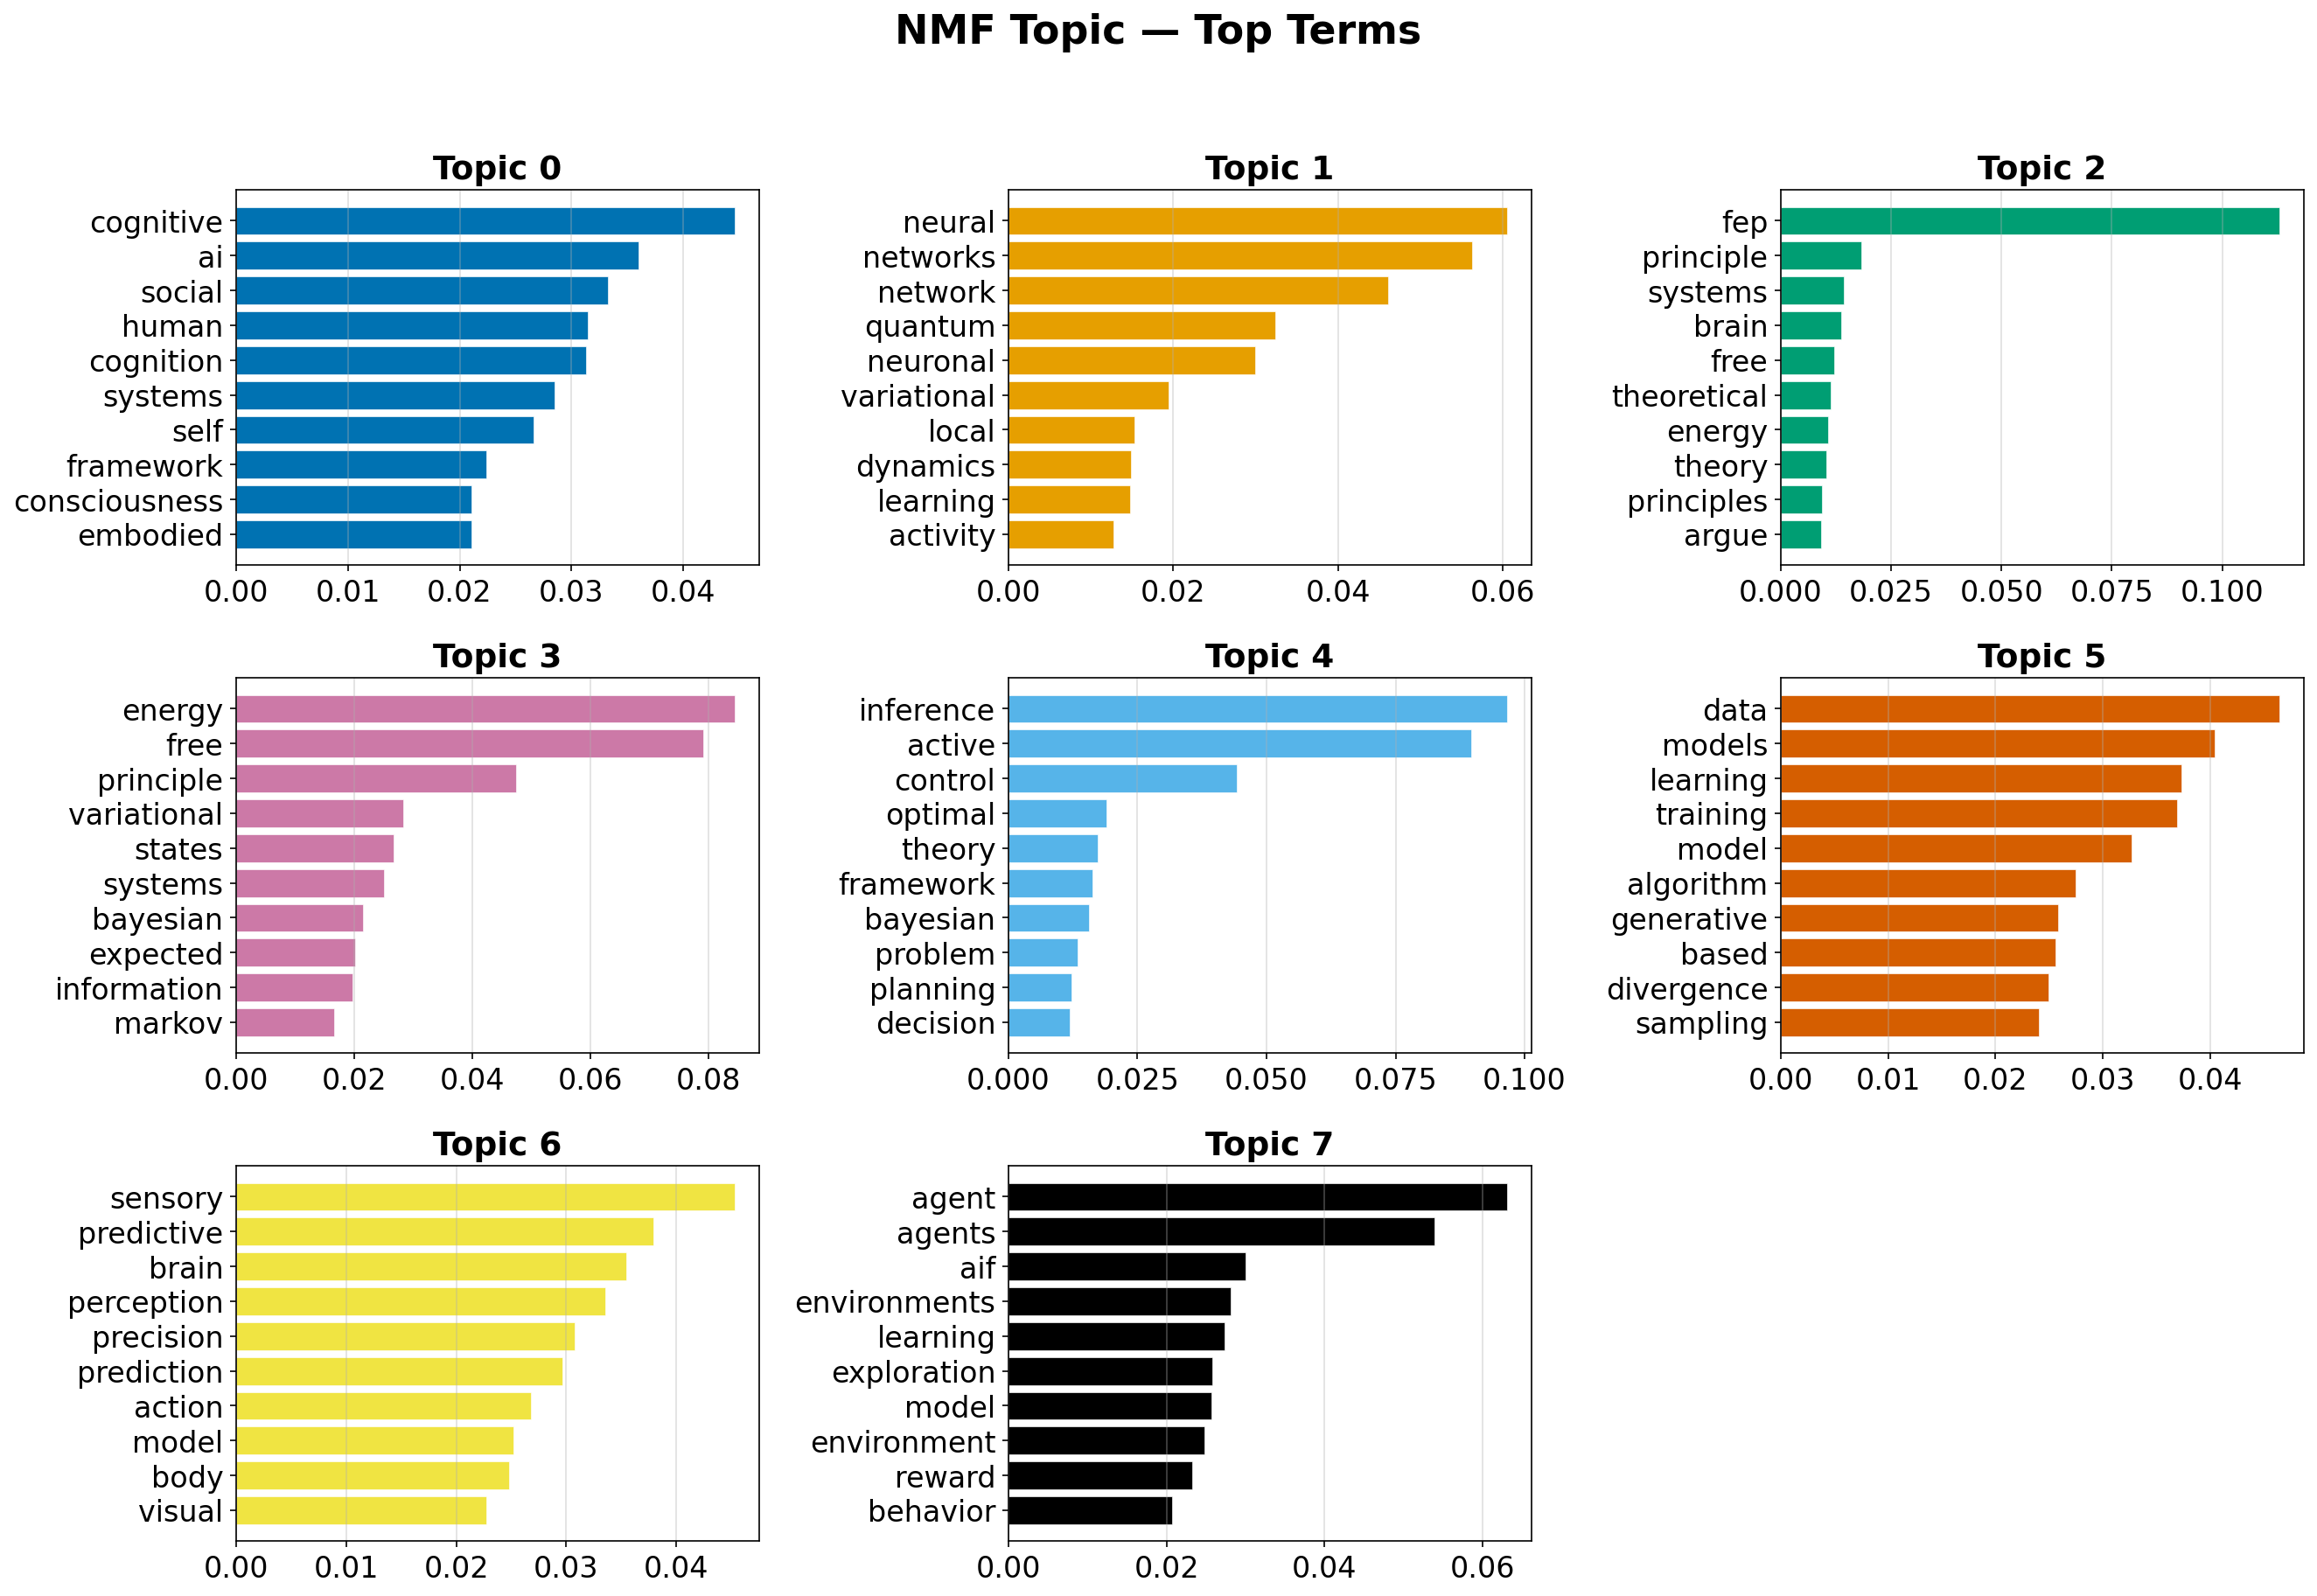
\includegraphics[width=0.9\textwidth]{../figures/topic_term_bars.png}
\caption{Top 10 terms per NMF topic ($k = 8$ topics, $500$ vocabulary features). Term weights reflect NMF component loadings; higher-weighted terms define each topic's semantic focus.}
\label{fig:topic_term_bars}
\end{figure}

\subsubsection{Vocabulary Analysis}\label{vocabulary-analysis}

\begin{figure}[htbp]
\centering
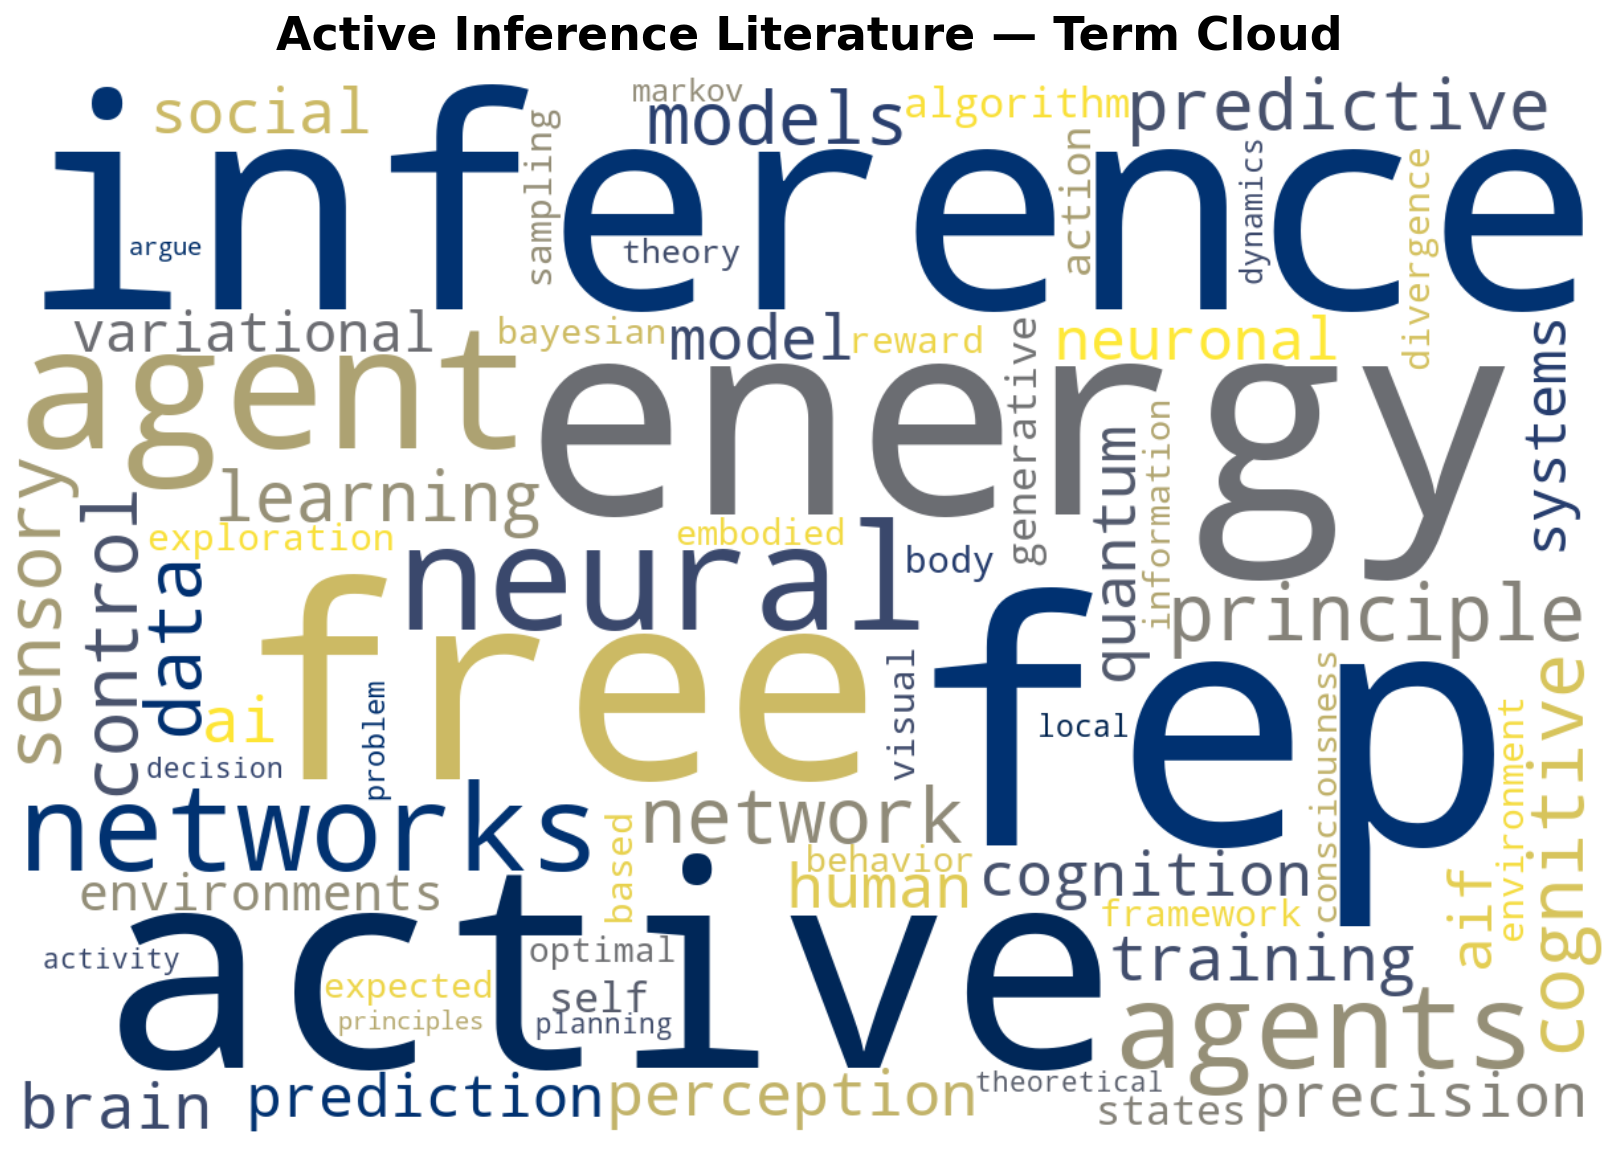
\includegraphics[width=0.9\textwidth]{../figures/word_cloud.png}
\caption{Word cloud of corpus vocabulary ($N = 1106$ abstracts) sized by maximum NMF component weight. Prominent terms—"inference," "active," "free energy," "model"—reflect the field's core theoretical commitments.}
\label{fig:word_cloud}
\end{figure}

The word cloud (Figure \ref{fig:word_cloud}) reveals the conceptual core
of the Active Inference literature: terms related to the Free Energy
Principle (``inference,'' ``active,'' ``free energy,'' ``model,''
``bayesian'') dominate, while application-specific terms appear at
smaller scales, reflecting the domain distribution's heavy A2
concentration.

\subsubsection{Document Embedding
Projections}\label{document-embedding-projections}

\begin{figure}[htbp]
\centering
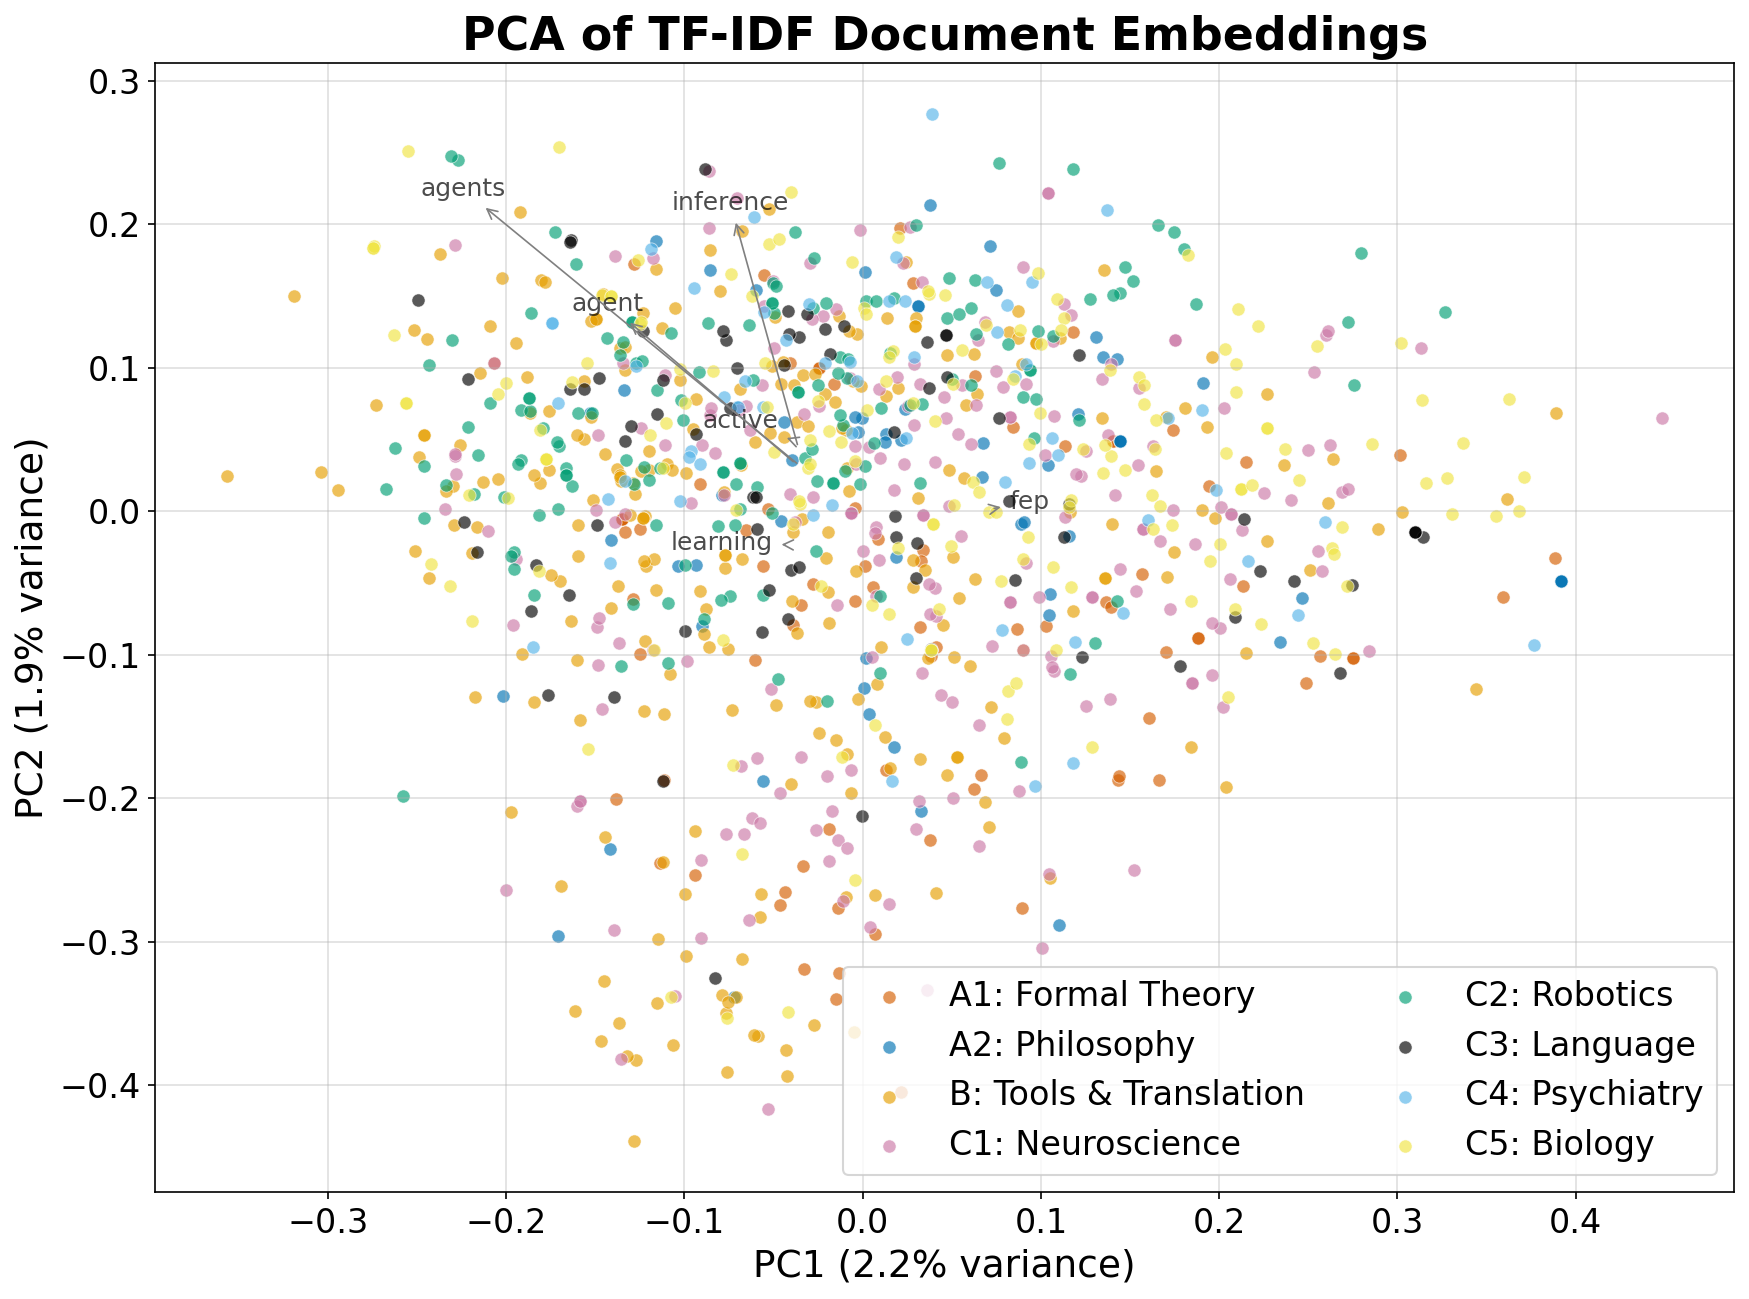
\includegraphics[width=0.9\textwidth]{../figures/pca_embeddings.png}
\caption{PCA projection of TF-IDF document embeddings ($N = 1106$ documents, $500$ features), colored by domain. Loading arrows indicate vocabulary terms contributing most to each principal component. Variance explained is annotated per axis.}
\label{fig:pca_embeddings}
\end{figure}

Principal Component Analysis of the TF-IDF document-term matrix projects
each paper into a two-dimensional space that preserves the directions of
maximum variance (Figure \ref{fig:pca_embeddings}). Rather than serving
solely as a visual clustering aid, this projection provides a
quantitative measure of semantic distance between subfields. The scatter
plot, colored by domain assignment, reveals the degree of semantic
separation between domains. Loading arrows overlay the top-variance
terms, showing which vocabulary drives the principal components and
highlighting the structural overlap between theoretically similar
domains that keyword-based hard categorization obscures.

\subsubsection{Domain Semantic
Similarity}\label{domain-semantic-similarity}

To further interrogate the latent semantic structure of the subfields,
we extract the top characterizing terms for each domain and compute a
hierarchical clustering of domain centroids. The heatmap (Figure
\ref{fig:term_heatmap}) reveals distinctive vocabulary patterns beyond
mere keyword-level classification, while the dendrogram (Figure
\ref{fig:dendrogram}) confirms the tight semantic proximity between Core
Theory subfields (A1, A2) and the close pairing of Tooling (B) with
Biology (C5).

\begin{figure}[htbp]
\centering
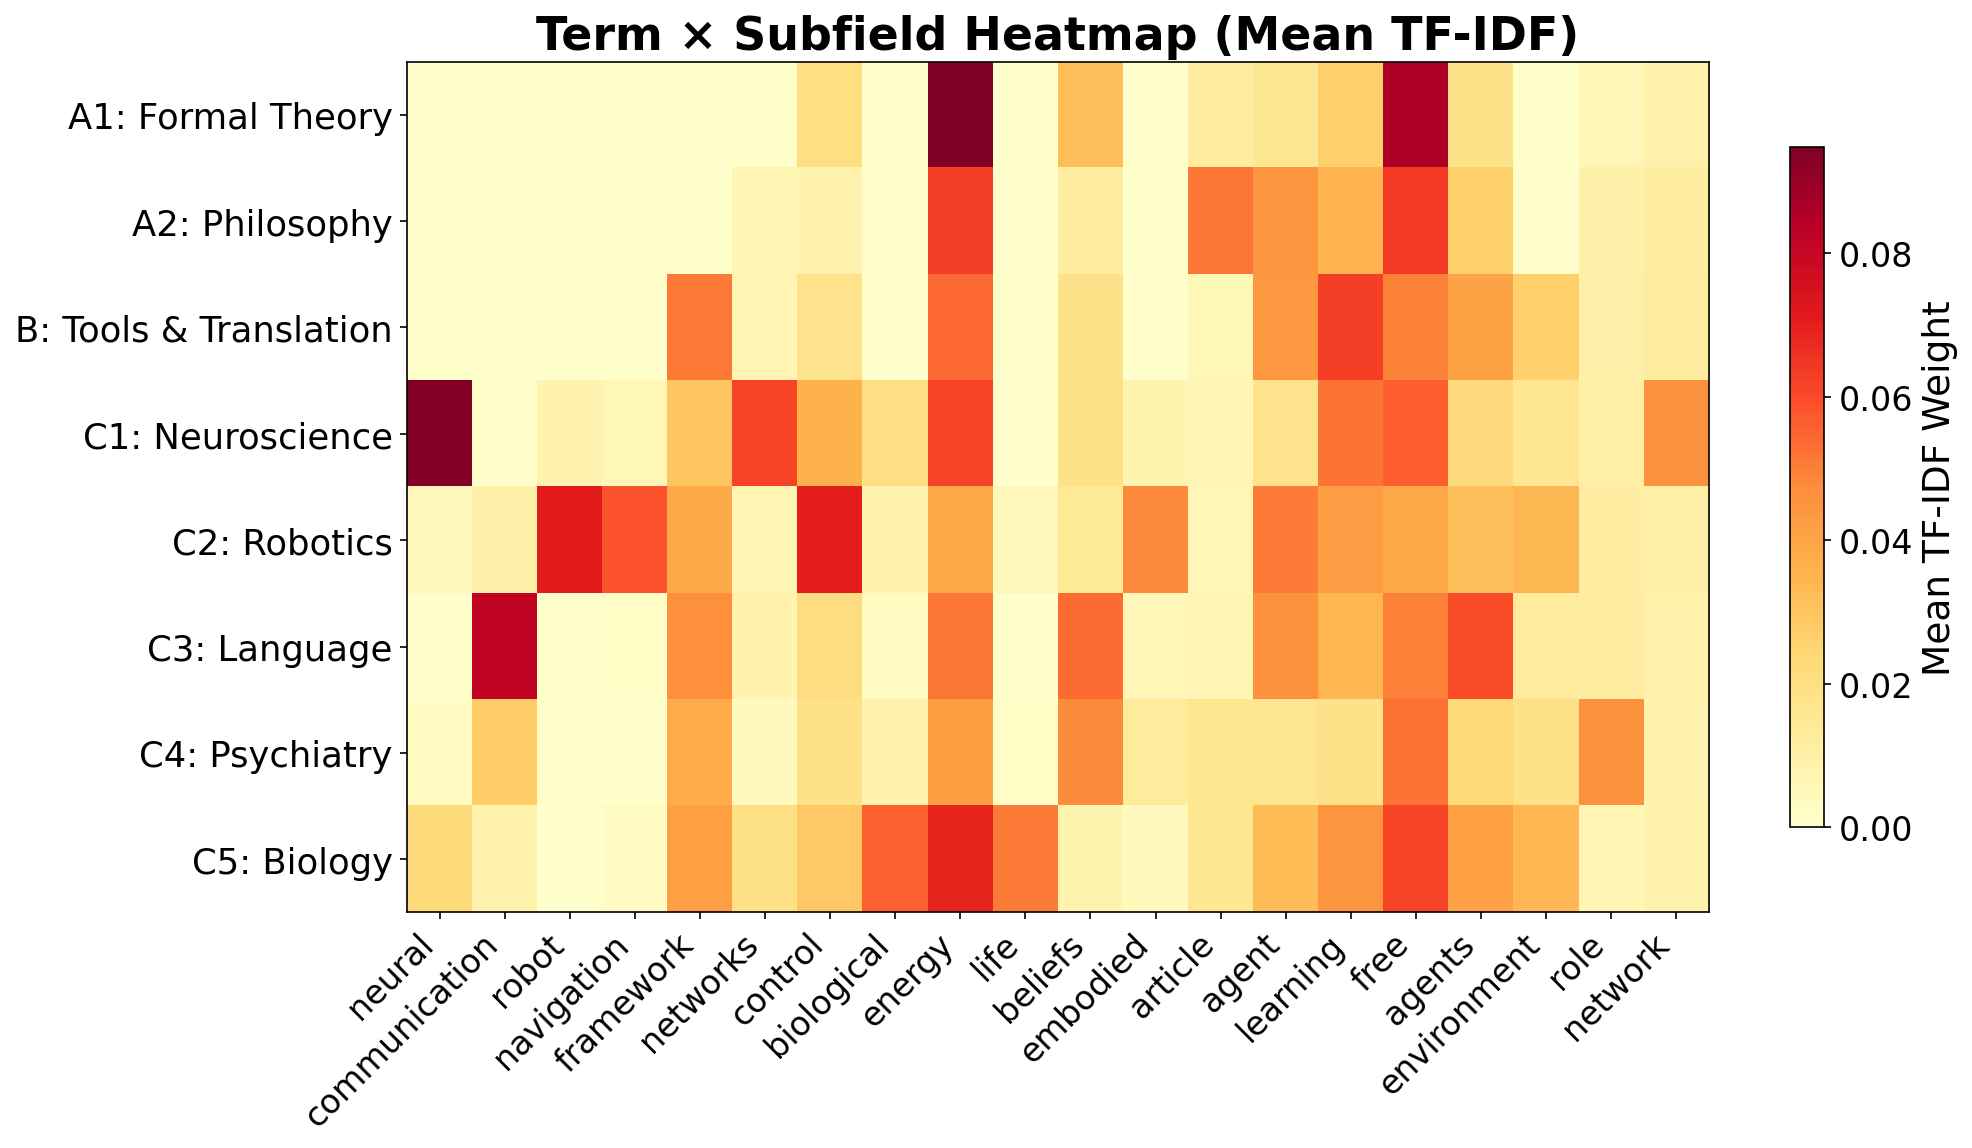
\includegraphics[width=0.9\textwidth]{../figures/term_heatmap.png}
\caption{Mean TF-IDF weight for the top 20 terms across all 8 domains. Darker cells indicate higher usage within a domain, revealing distinctive vocabulary patterns beyond the keyword-level classification used for subfield assignment.}
\label{fig:term_heatmap}
\end{figure}

\begin{figure}[htbp]
\centering
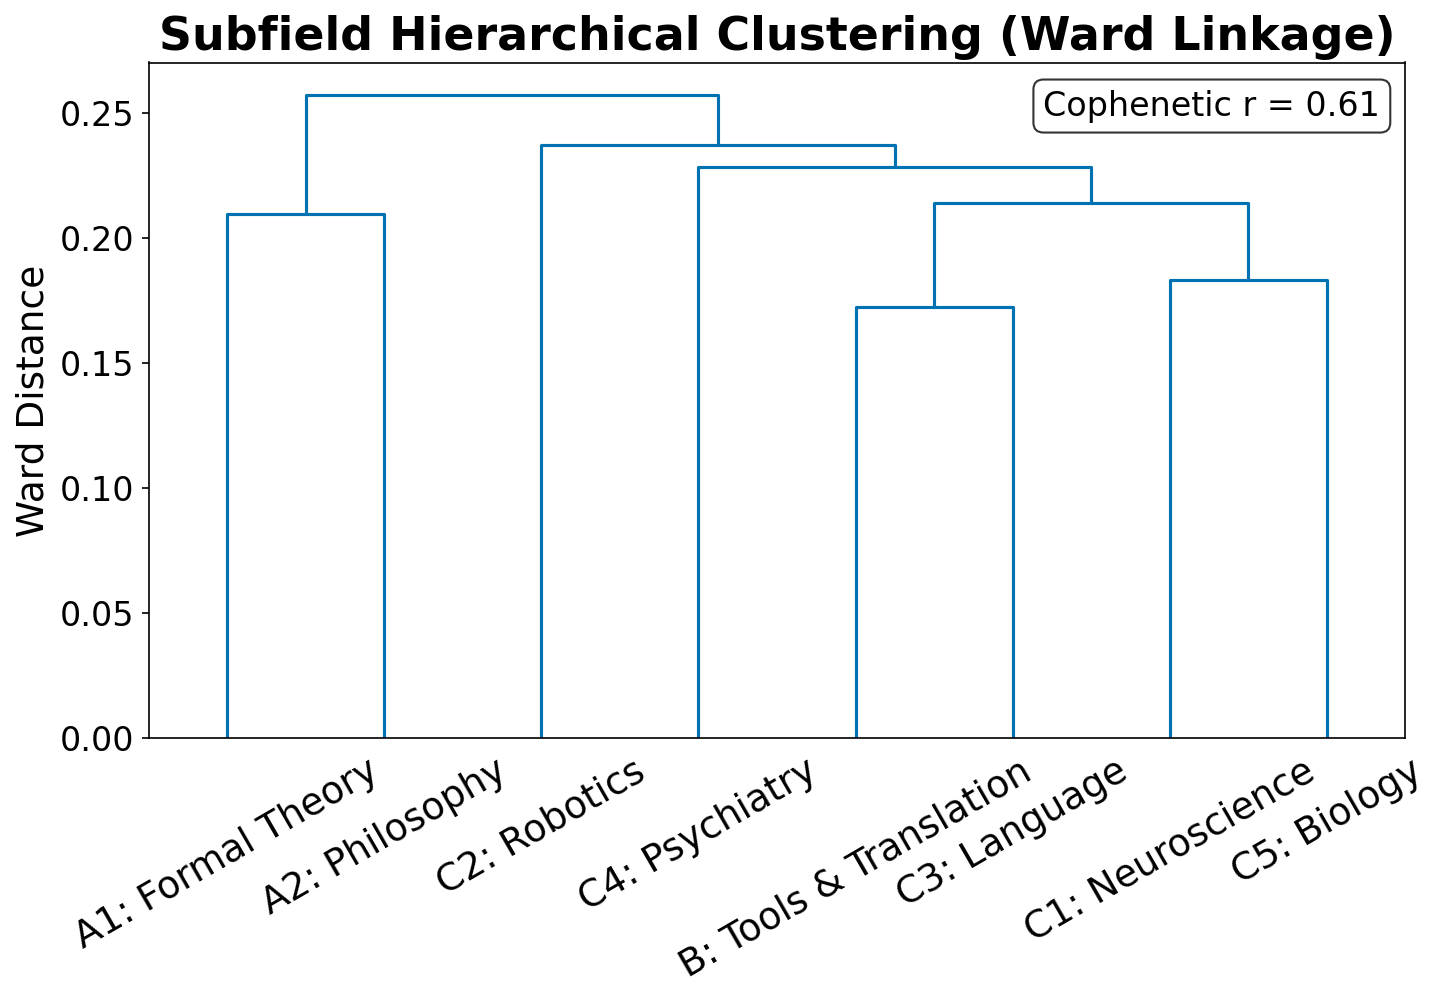
\includegraphics[width=0.9\textwidth]{../figures/dendrogram.png}
\caption{Hierarchical clustering of domain centroids (Ward linkage on mean TF-IDF vectors, 8 domains). Cophenetic correlation annotated on figure. A1 (formal theory) and A2 (philosophy) cluster closely, as do B (tools) and C5 (biology); C4 (psychiatry) groups with the core-theory pair rather than with the other application domains.}
\label{fig:dendrogram}
\end{figure}

\subsubsection{Term Co-occurrence
Patterns}\label{term-co-occurrence-patterns}

\begin{figure}[htbp]
\centering
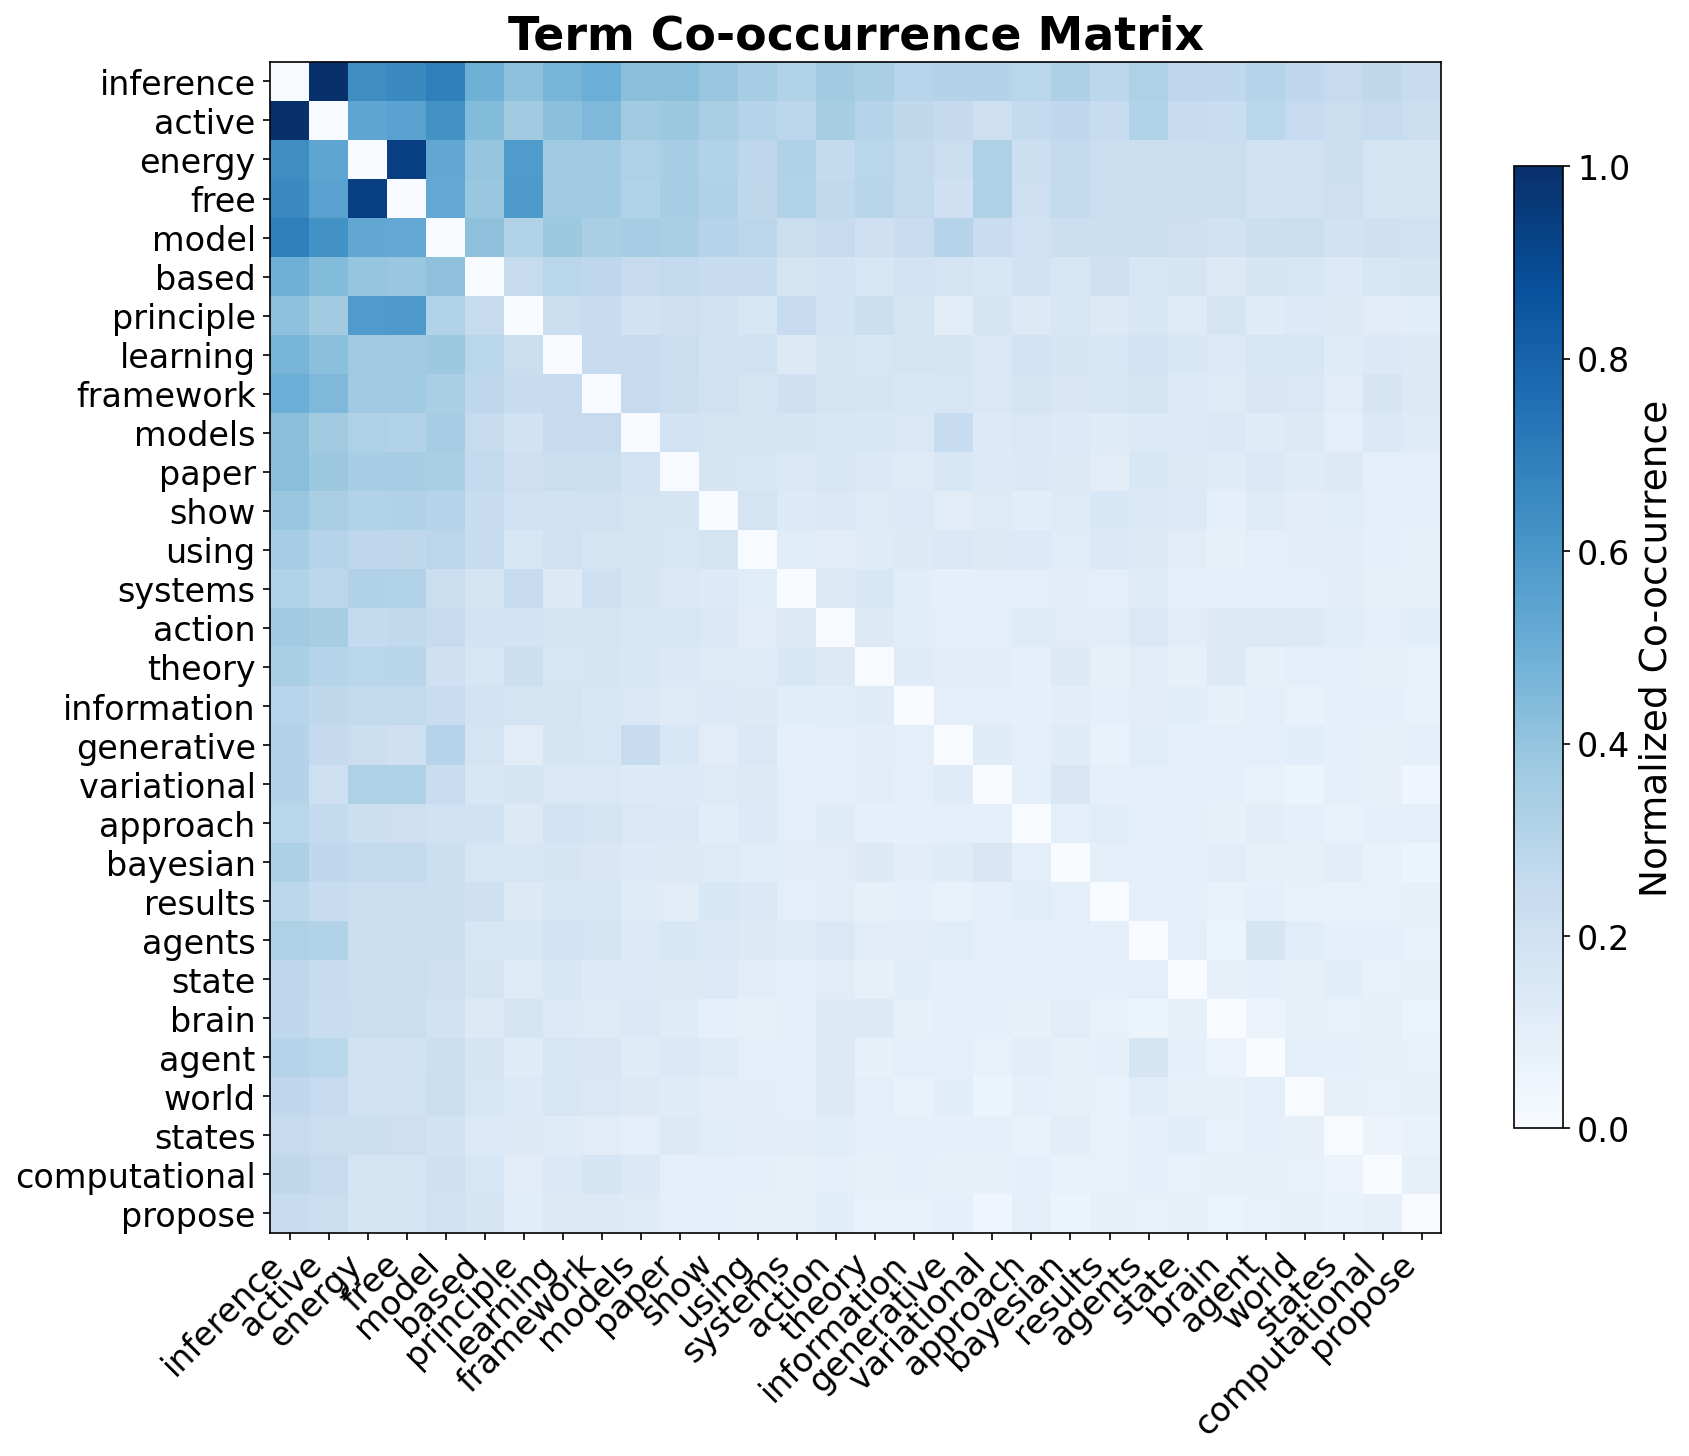
\includegraphics[width=0.9\textwidth]{../figures/cooccurrence_matrix.png}
\caption{Normalized co-occurrence matrix for the 30 most frequent terms across $N = 1106$ abstracts. Cell intensity reflects the fraction of documents in which two terms co-appear, normalized to $[0, 1]$.}
\label{fig:cooccurrence_matrix}
\end{figure}

The co-occurrence matrix (Figure \ref{fig:cooccurrence_matrix}) for the
30 most frequent corpus terms reveals tightly coupled term clusters
corresponding to the NMF topics. The strong co-occurrence between
``free,'' ``energy,'' ``principle,'' and ``bayesian'' anchors the
theoretical core, while application-specific term clusters (e.g.,
``brain''--``cognitive''--``predictive''--``coding'') form distinct
off-diagonal blocks. The relative isolation of robotics-specific terms
from neuroscience terms confirms the semantic separation between these
application domains despite their shared theoretical foundation.

\newpage

\subsection{Citation Network Topology}\label{sec:citation_network}

The intra-corpus citation network provides a structural view of how
Active Inference research is organized, identifying influential hub
papers, community structure, and patterns of citation isolation (Figure
\ref{fig:citation_network}).

\begin{figure}[htbp]
\centering
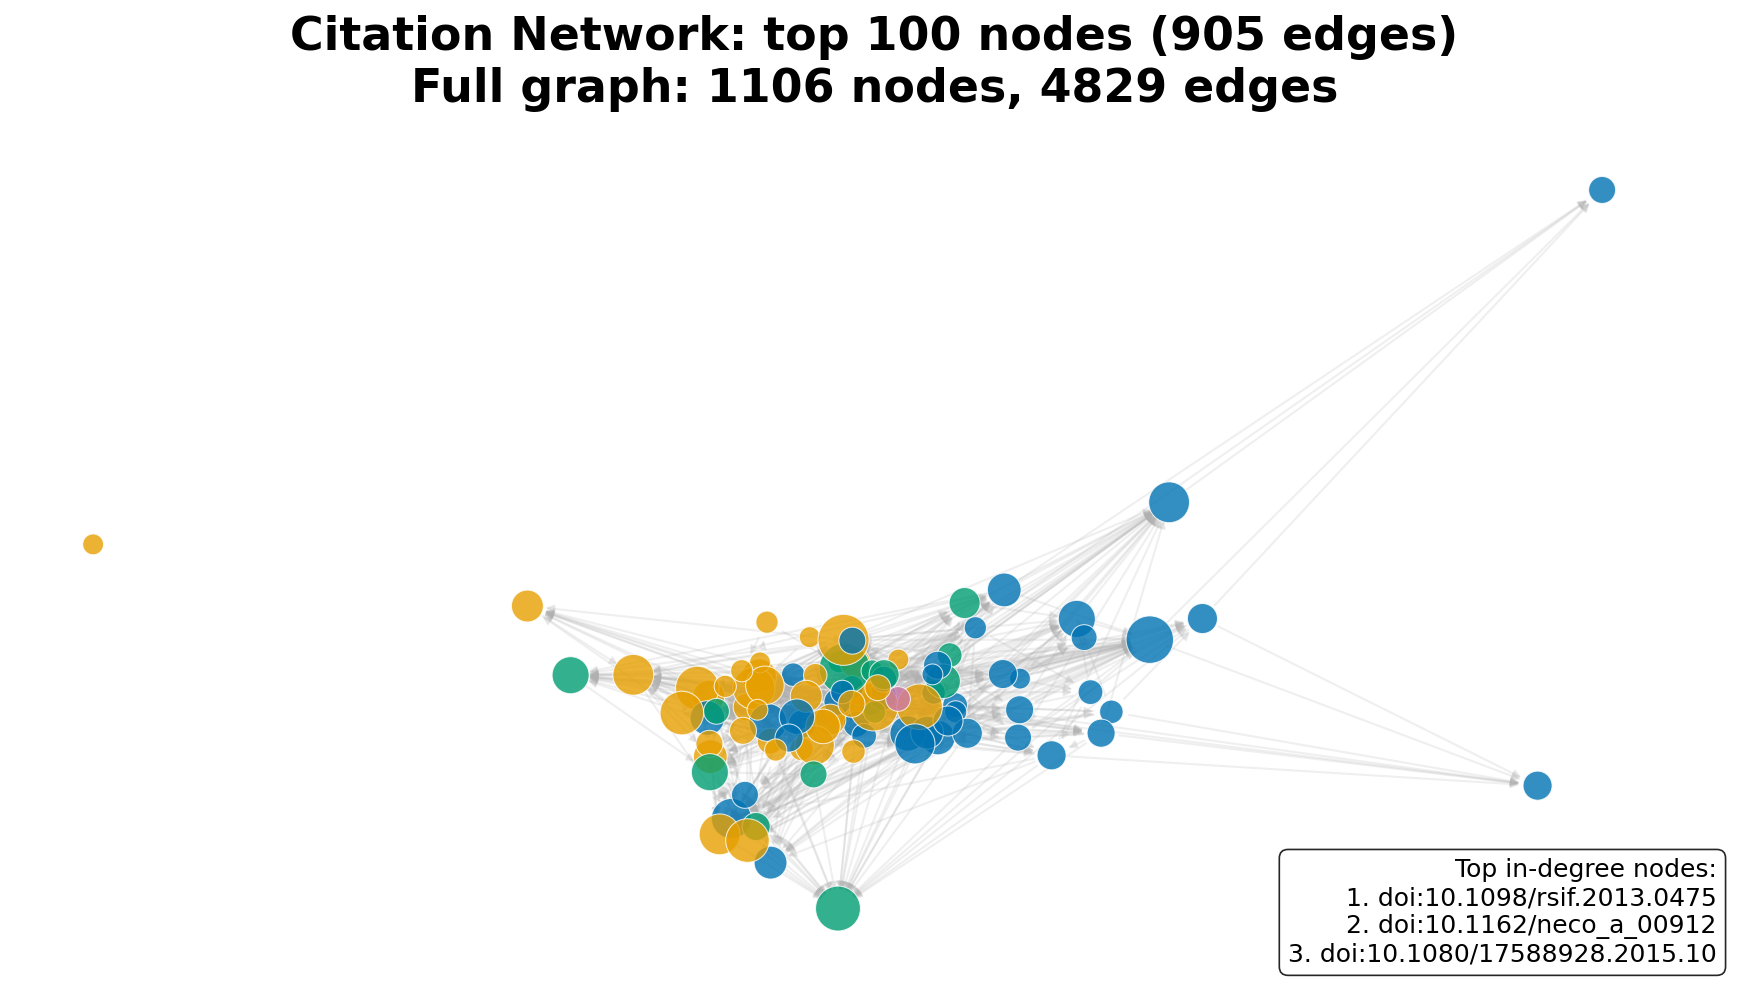
\includegraphics[width=0.9\textwidth]{../figures/citation_network.png}
\caption{Intra-corpus citation network. The figure shows a 100-node view (905 edges) of the full graph (1106 nodes, 4,829 edges); node size reflects in-degree and highly cited foundational papers serve as nexus points connecting sub-domains.}
\label{fig:citation_network}
\end{figure}

\subsubsection{Network Density and Degree
Distribution}\label{network-density-and-degree-distribution}

The intra-corpus citation network contains 1106 nodes and 4,829 edges,
with a density of 0.40\% and 645 connected components. The average
in-degree of approximately 4.4 indicates that most papers receive few
intra-corpus citations, consistent with the field's rapid expansion: the
majority of recent papers have not yet accumulated citations within the
corpus (Figure \ref{fig:degree_distribution}). Only 10.4\% of all
identified references (4,829 intra-corpus matches out of 46,598 total
reference entries) resolve to other papers within the corpus, reflecting
cross-source identifier mismatches and the field's engagement with a
broad external literature base. Community detection identifies clusters
via greedy modularity maximization \citep{clauset2004finding}.

\begin{figure}[htbp]
\centering
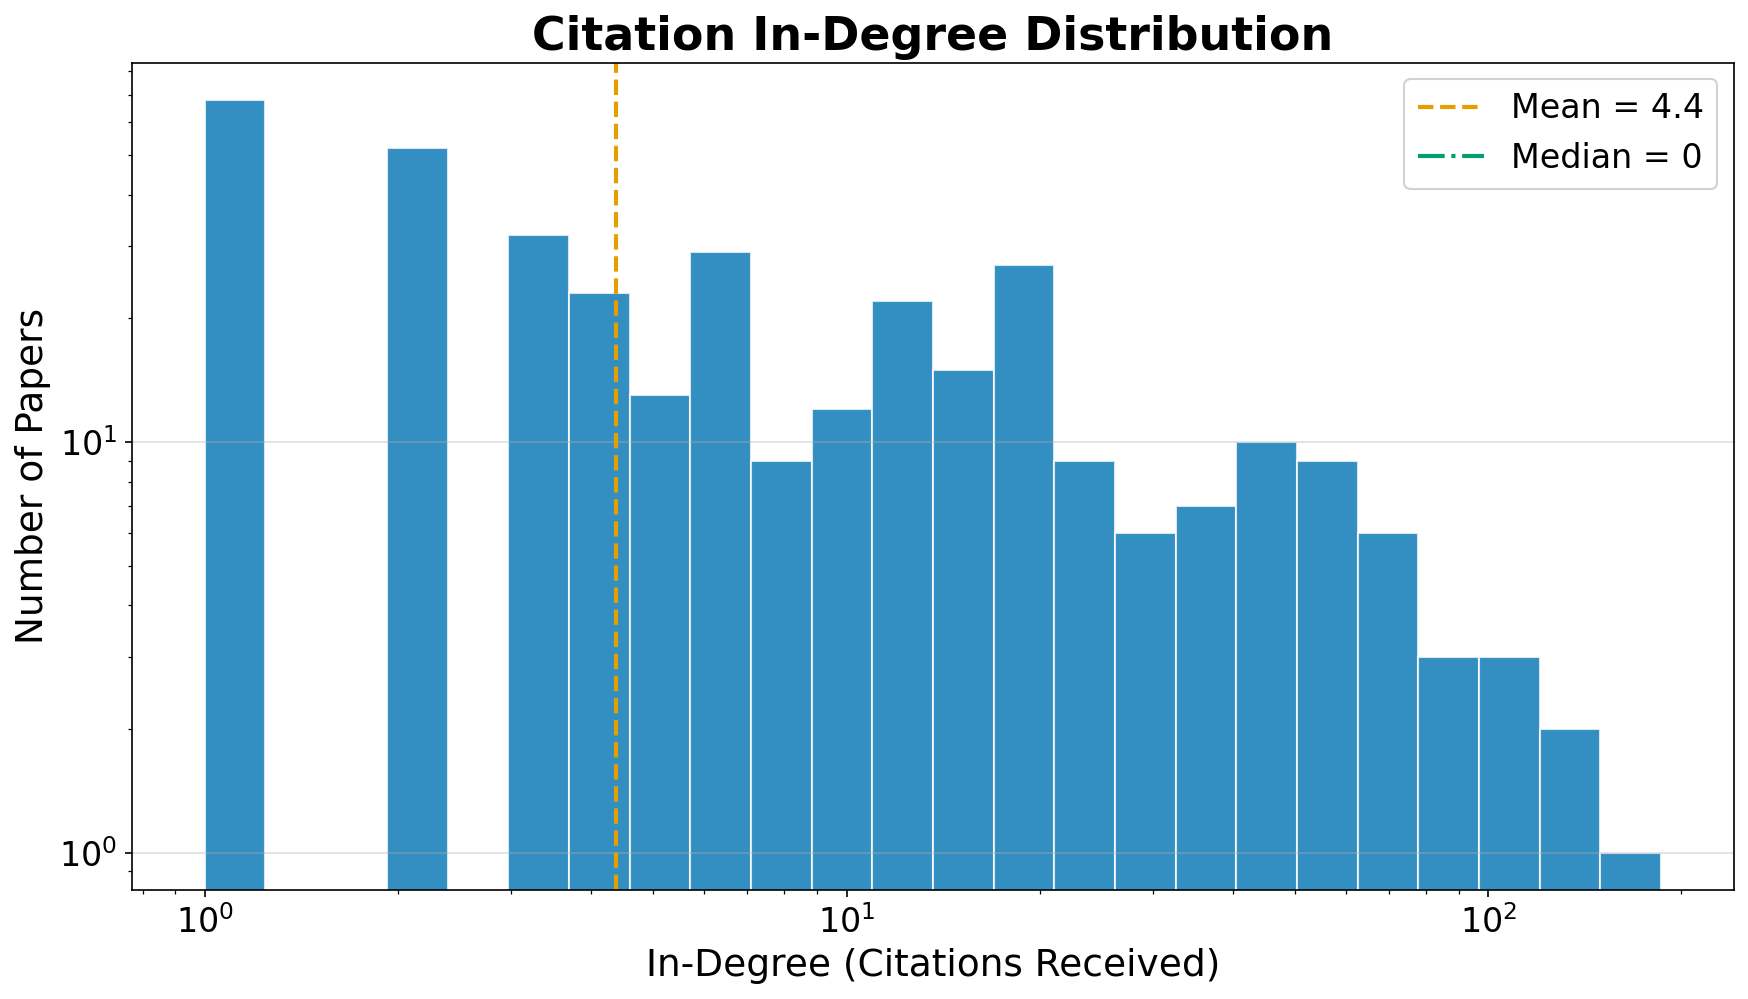
\includegraphics[width=0.7\textwidth]{../figures/degree_distribution.png}
\caption{In-degree distribution of the citation network. The power-law tail is characteristic of citation networks, with a small number of highly cited hubs.}
\label{fig:degree_distribution}
\end{figure}

\subsubsection{Connected Components and Citation
Isolation}\label{connected-components-and-citation-isolation}

The high number of connected components (645 out of 1106 nodes) reveals
that much of the corpus consists of citation-isolated papers---works
that neither cite nor are cited by other papers in the collection. A
single Giant Connected Component (GCC) typically dominates mature
scientific networks; here, with 645 components across 1106 nodes, the
GCC contains a minority of nodes while the remainder form singletons or
small clusters of two to three papers. This is partially an artifact of
cross-source identifier mismatches, but it also reflects the field's
pattern of papers engaging with the FEP literature conceptually without
building explicit, graph-tractable citation chains. PageRank analysis
identifies highly influential papers, predominantly Friston's
foundational work \citep{friston2010free} and the AIF textbook
\citep{parr2022active}, which serve as nexus points linking otherwise
disconnected subgraphs.

\subsubsection{Network Summary}\label{network-summary}

\begin{table}[htbp]
\centering
\caption{Intra-corpus citation network summary statistics ($N = 1106$ papers, 1106 nodes). The low density and high component count reflect the field's rapid expansion and cross-source identifier mismatches.}
\label{tab:citation_network}
\begin{tabular}{ll}
\toprule
\textbf{Metric} & \textbf{Value} \\
\midrule
Nodes & 1106 \\
Edges & 4,829 \\
Reference resolution rate & 10.4\% (4,829 / 46,598) \\
Connected components & 645 \\
Network density & 0.40\% \\
Mean in-degree & approximately 4.4 \\
\bottomrule
\end{tabular}
\end{table}

The citation topology corroborates the field overview findings (RQ1,
RQ2): a small number of foundational papers---predominantly Friston's
free energy and active inference formulations---anchor a rapidly
expanding periphery of increasingly specialized work. The extremely low
density (0.40\%) corresponds to an epistemic stage of high
fragmentation, meaning that literature synthesis and cross-pollination
between specific sub-domains remain difficult. Theoretical influence
flows primarily through shared conceptual foundations (the hub nodes)
rather than through dense mutual citation across the periphery. As
metadata standardization improves and DOI adoption becomes universal
across preprint and journal ecosystems, re-running this pipeline should
yield substantially higher reference resolution rates and a more
connected graph, enabling finer-grained community detection and
tracking.

\newpage

\section{Conclusion: Evidence Landscape, Methodological Limitations, and
Research Agenda}\label{sec:conclusion}

\subsection{Summary}\label{summary}

This work demonstrates a first-generation prototype infrastructure for
citation-weighted evidence mapping and hypothesis triage across a
rapidly growing scientific field. By combining configured multi-source
retrieval (\(N = 1106\) papers, inclusion from 2000 onward; arXiv,
OpenAlex completed; Semantic Scholar incomplete), LLM-based assertion
extraction encoded as provenance-bearing nanopublications, and
citation-weighted triage scoring, we produce a queryable, RDF-compatible
knowledge graph that maps the evolving evidence landscape for eight core
Active Inference claims. The system demonstrates the feasibility of
automated living reviews, while clearly delineating the boundaries of
current model capabilities.

All assertions and hypothesis scores are machine-generated; outputs
always report evidence mapping and triage, not scientific
confirmation---there is no live gate that suppresses or changes output
based on the validation metrics below, which are reported as
reproducibility context, not an enforced pass/fail threshold. A
stratified rule-based reference-annotator agreement study (\(n = 256\))
yields inter-rule \(\kappa = 0.704\) and pipeline precision 0.013,
recall 1.000 against a deterministic keyword-rule reference; direction
agreement between that reference and the pipeline is only
\(\kappa = -0.048\). These are reproducibility signals, not accuracy
against human labels---the pre-declared human gold-standard baseline
below has not yet been collected.

\subsection{Constraints and Methodological
Scope}\label{constraints-and-methodological-scope}

Several conscious design constraints scope these findings.

\subsubsection{Keyword Classifier
Resolution}\label{keyword-classifier-resolution}

The keyword-based classifier operates over 200+ keyword indicators
distributed across 8 domain categories (74 mathematical indicators in A1
alone), using a deterministic priority system that routes papers to
specific application domains (C1--C5) before testing tools (B), formal
theory (A1), and the qualitative philosophy catch-all (A2).
Word-boundary-aware matching reduces partial-match false positives, but
keyword-based methods cannot capture semantic nuance: papers using novel
terminology or discussing cross-domain topics without standard
vocabulary risk misclassification. Residual A2 concentration should be
interpreted as a ceiling on broad theoretical generality rather than a
literal measure of philosophical focus. An embedding-based classifier
trained on a labeled subset would provide a quantitative upper bound on
the fraction of A2 papers that merit redistribution.

\subsubsection{Citation Network Coverage
Gaps}\label{citation-network-coverage-gaps}

The 4,829 intra-corpus edges spanning 645 connected components provide a
topological skeleton, but three systematic gaps inflate the component
count: (1) cross-source identifier mismatches (DOI vs.~OpenAlex
vs.~arXiv ID), (2) papers whose references are not indexed by any source
API, and (3) open-access preprints whose DOIs differ from their
published versions. Exhaustive DOI-level cross-matching with fuzzy title
matching would condense the graph further.

\subsubsection{Corpus Biases, Citation Dynamics, and Linguistic
Framing}\label{corpus-biases-citation-dynamics-and-linguistic-framing}

Citation counts are subject to Matthew effects and cumulative field-size
biases. Partial-year indexing for the most recent calendar year
undercounts recent publications. The measured 24.94\% CAGR is calculated
over complete years 2003--2025, while 98 papers from 2026 are reported
as of 2026-07-26 and excluded from that endpoint. Additionally, the
retrieved corpus itself suffers from selection biases inherent to
queried databases, including English-language dominance and the
structural over-indexing of preprints relative to peer-reviewed final
versions. Finally, positive and negative hypothesis scores alike are
affected by publication bias and linguistic asymmetry: declarative
scholarly claims are phrased affirmatively more often than negatively.
Relative rankings and temporal trajectories are retained for transparent
comparison, but their robustness is not established by this
abstract-only calibration.

\subsubsection{LLM Extraction Fidelity, Domain Drift, and
Robustness}\label{llm-extraction-fidelity-domain-drift-and-robustness}

Zero-shot LLM extraction introduces distinct systematic biases:
over-extraction (the model hallucinating certainty for claims the paper
merely mentions in passing) and direction inversion (misclassifying
opposing evidence as supporting). Recent benchmarking confirms that
state-of-the-art systems often fall short of production-level precision
on tasks requiring exhaustive retrieval and aggregation of directional
claims from long documents \citep{liang2024survey}. Furthermore, because
our corpus extends to 2026, LLM extraction is vulnerable to \emph{domain
drift}---the base models may lack parametric knowledge of the most
recent theoretical developments. As an alternative, fine-tuned models
specifically trained on FEP/AIF abstracts could yield higher precision
than our zero-shot approach, though at a steeper computational setup
cost.

The current validation protocol is a deterministic rule-based reference
study, not a human-annotation ground truth. It provides a
reproducibility floor through inter-rule agreement and
pipeline-versus-reference metrics; a future human-labeled study is
required before making accuracy claims.

\subsection{Research Agenda: Four Priority Next
Steps}\label{sec:next_steps}

The current prototype establishes a reproducible baseline and surfaces
the field's evidence structure at corpus scale. Four concrete next
steps, ordered by the dependency chain each one unlocks, define the path
from prototype to production-grade living review.

\subsubsection{Next Step 1 --- Expand the Scope of Referenced
Data}\label{next-step-1-expand-the-scope-of-referenced-data}

The present corpus of \(N = 1106\) papers is assembled via keyword
queries against the configured APIs (Semantic Scholar, OpenAlex, arXiv);
this snapshot records arXiv, OpenAlex completed; Semantic Scholar
incomplete. Three expansion axes would materially change the evidence
landscape.

\textbf{Additional sources.} PubMed, PsycINFO, and IEEE Xplore each
index Active Inference literature that the current APIs do not reach:
neuroscience clinical trials (PubMed), cognitive-behavioral studies
(PsycINFO), and robotics control architectures (IEEE). For each new
source, the retrieval layer requires only a source-specific connector
implementing the same \breaktt{fetch\_papers(query,\ max\_results)}
interface used by existing adapters. Gray literature---technical
reports, theses, and institutional preprints not yet indexed by major
APIs---represents an additional tier: harvesting from ORCID work records
and institutional repositories would capture practitioner findings that
never appear in indexed venues.

\textbf{Broader query coverage.} The current query set is derived from
the eight hypothesis keywords and their immediate synonyms. Expanding to
a full ontological synonym set (e.g., mapping ``variational inference,''
``surprise minimization,'' and ``Helmholtz machine'' as equivalent
retrieval terms for FEP-related claims) would reduce the retrieval
false-negative rate for papers that use non-canonical vocabulary. A
systematic evaluation of retrieval precision and recall against a
hand-curated gold-standard set of 100 known AIF papers would quantify
the gap.

\textbf{Custom curated bibliographies.} Domain experts can contribute
citation lists directly to the corpus without modifying any code:
placing a \texttt{.bib} or \texttt{.ris} file in
\breaktt{data/custom\_bibliographies/} triggers the deduplication merge
on the next pipeline run. This pathway is the lowest-friction route to
extending scope for researchers who maintain personal reference
libraries.

\subsubsection{Next Step 2 --- Extract and Verify Evidence Supporting
Claims in Each
Paper}\label{next-step-2-extract-and-verify-evidence-supporting-claims-in-each-paper}

The current extraction pipeline operates exclusively on abstracts.
Abstracts contain the claims authors choose to foreground, not
necessarily the claims best supported by the paper's data. Three
mechanisms bridge this gap.

\textbf{Full-text ingestion.} For the subset of papers with open-access
PDFs (approximately 60--70\% of recent AIF preprints on arXiv), Stage 3
can be extended to parse full-text sections---specifically Methods,
Results, and Discussion---using a structured chunking strategy that
splits documents into about 512-token segments aligned to
section boundaries. The existing nanopublication schema accommodates a
\texttt{source\_section} field (currently unused) that would record the
provenance of each extracted assertion (abstract vs.~results
vs.~discussion), enabling downstream stratification of evidence by
rhetorical function.

\textbf{Claim-evidence pairing.} The current extraction prompt asks the
LLM to classify a paper's stance toward a hypothesis but does not
require it to quote the specific sentence or data point that justifies
the classification. A revised prompt would require the model to (a)
identify the hypothesis-relevant passage verbatim, (b) classify the
stance, and (c) rate confidence on the basis of whether the passage
reports an empirical measurement, a theoretical derivation, or an
assertion without quantitative support. This three-field extraction ---
\texttt{evidence\_quote}, \texttt{stance}, \texttt{evidence\_type} ---
upgrades the nanopublication from a classification label to a traceable
evidential pointer. For H3 (Markov Blanket Realism), where the 14
contradicting assertions drive a contested score, reviewers could then
inspect the actual quoted passages rather than trusting the LLM
classification in isolation.

\textbf{Human spot-check coverage.} The planned 10\% manual-annotation
baseline would focus on inter-rater agreement; this manual validation
has not yet been performed. Extending spot-checks to verify that the
extracted evidence quote actually appears in the source document (a
verbatim-match check) adds an additional fidelity gate beyond stance
accuracy.

\subsubsection{Next Step 3 --- Tie Hypotheses to Real-World
Outcomes}\label{next-step-3-tie-hypotheses-to-real-world-outcomes}

The eight tracked hypotheses are formulated at the level of theoretical
constructs (e.g., ``the FEP provides a universal account of
self-organizing systems''). Practical applicability requires mapping
from hypothesis support to observable real-world outcomes,
distinguishing which claims are actionable from which remain theoretical
scaffolding.

\textbf{Outcome taxonomy.} Each hypothesis should be annotated with a
set of \emph{outcome indicators}: specific, measurable real-world
results whose observation would constitute evidence for or against the
hypothesis under the closest empirical operationalization. For example:
- H4 (Predictive Coding): outcome indicator = reduction in
prediction-error amplitude as measured by ERP N400 or oscillatory
gamma-band response in human neuroimaging studies. - H5 (Scalability):
outcome indicator = task performance on standard RL benchmarks (Atari,
MuJoCo, ProcGen) at or above the performance of model-free SOTA at
matched computational budgets. - H6 (Clinical Utility): outcome
indicator = statistically significant improvement on standardized
psychiatric assessment scales (PANSS, BDI-II, PTSD Checklist) in at
least one registered clinical trial. - H7 (Morphogenesis): outcome
indicator = quantitative recapitulation of at least one morphogenetic
patterning sequence (e.g., digit formation timecourse, limb bud size
scaling) in a computational model governed by FEP dynamics rather than
reaction-diffusion equations.

For each hypothesis, the extraction pipeline can be extended to tag
assertions whose evidence type is \breaktt{empirical\_measurement} and
whose outcome aligns with these indicators, producing a filtered score
that counts only outcome-linked evidence. This \emph{outcome-filtered
score} sits alongside the current citation-weighted score in the
hypothesis table, providing a direct answer to ``how much of this
support is grounded in real-world observations rather than theoretical
commentary?''

\textbf{Application domain cross-walk.} The subfield classification
(A1--C5) already partitions the corpus by application domain.
Intersecting hypothesis scores with application domain
membership---computing \(\text{score}(H_i, D_j)\) for each hypothesis
\(H_i\) and domain \(D_j\)---would reveal which domains are generating
empirical traction versus theoretical citation counts. H1 (FEP
Universality) likely has high A2 (philosophy) support and lower C1--C5
empirical support; quantifying this split would replace qualitative
description of the ``neutral plurality'' with a decomposed evidence
profile grounded in domain labels already computed by Stage 2.

\subsubsection{Next Step 4 --- Formal Evaluation Rubric for Pipeline
Quality}\label{next-step-4-formal-evaluation-rubric-for-pipeline-quality}

The current validation is primarily structural: do scripts run, do
outputs exist, do tests pass, does the PDF render? A formal evaluation
rubric answers a different question: \emph{how accurate is the evidence
landscape this system produces?} Four rubric dimensions, together with
their measurement protocols and target thresholds, define what ``good
enough for a published living review'' means.

\begin{table}[htbp]
\centering
\caption{Proposed evaluation rubric for pipeline quality assessment. Each dimension has a measurement protocol, a current baseline, and a target threshold for a production living review. All metrics are computed on a held-out annotation set of 200 randomly sampled assertions.}
\label{tab:eval_rubric}
\begin{tabular}{llll}
\toprule
\textbf{Dimension} & \textbf{Protocol} & \textbf{Current} & \textbf{Target} \\
\midrule
Extraction direction accuracy & Cohen's $kappa$ (rule reference vs.\ LLM stance) & $kappa = -0.048$ & $kappa > 0.80$ \\
Evidence-quote fidelity & Verbatim substring match rate & 0.053 (no quotes stored) & $>= 90\%$ \\
Corpus recall & Precision/recall vs.\ rule reference & $P = 0.013$, $R = 1.000$ & recall $>= 0.85$ \\
Outcome grounding rate & Fraction of supporting assertions citing an outcome indicator & pending & $>= 30\%$ \\
\bottomrule
\end{tabular}
\end{table}

The four rubric dimensions map directly to the four next steps: corpus
recall measures Step 1 progress, evidence-quote fidelity measures Step 2
progress, outcome grounding rate measures Step 3 progress, and
extraction direction accuracy is the targeted baseline to be established
as the other three improve. Reporting all four numbers alongside
hypothesis scores in each pipeline release converts a qualitative
description of limitations into a versioned, trackable quality
scorecard. This transforms the current ``we acknowledge limitations''
posture into an audit trail: readers can see whether the rubric scores
improved between release v1.0 and v2.0, and reviewers can evaluate
pipeline trustworthiness on principled criteria rather than subjective
judgement.

\begin{center}\rule{0.5\linewidth}{0.5pt}\end{center}

\subsection{Future Directions: Beyond Tally-Based Evidence
Aggregation}\label{future-directions-beyond-tally-based-evidence-aggregation}

Beyond the four priority next steps above, the scoring machinery itself
can be upgraded. We identify four directions, ordered by expected
impact.

\subsubsection{Hierarchical Bayesian Hypothesis
Scoring}\label{hierarchical-bayesian-hypothesis-scoring}

The most direct extension replaces the additive tally with a
\textbf{hierarchical Bayesian model} that treats each hypothesis score
as a latent variable inferred from noisy assertion observations. Under
this formulation, each assertion \(a_i\) contributes a likelihood term
\(P(a_i | \theta_H, \sigma)\) parameterized by the hypothesis-level
evidence strength \(\theta_H\) and an observation noise term \(\sigma\)
capturing LLM extraction uncertainty. A hierarchical prior
\(\theta_H \sim \mathcal{N}(\mu_{\text{field}}, \tau^2)\) pools
information across hypotheses, enabling principled shrinkage for
hypotheses with sparse evidence (e.g., H6 Clinical Utility, with only 26
assertions). This framework produces posterior credible intervals rather
than point estimates, providing uncertainty quantification that the
current tally-based scores lack. Temporal dynamics can be modeled
through time-varying parameters \(\theta_H(t)\) using state-space
formulations that re-weight older evidence rather than treating all
cumulative assertions equally.

\subsubsection{Causal Evidence Graphs}\label{causal-evidence-graphs}

A second-generation knowledge graph would encode not only
assertion-level relationships (paper \texorpdfstring{\ensuremath{\to}}{->} supports \texorpdfstring{\ensuremath{\to}}{->} hypothesis) but also
\textbf{causal dependencies among hypotheses} themselves. For example,
evidence for predictive coding (H4) often implicitly supports FEP
universality (H1), yet the tally-based approach treats them as
independent. A causal evidence graph---structured as a directed acyclic
graph (DAG) over hypotheses with edge weights learned from co-assertion
patterns---would enable cross-hypothesis evidence propagation using
belief propagation or variational message passing. This is particularly
relevant for the Active Inference literature, where hypotheses are
theoretically nested: FEP universality (H1) logically entails predictive
coding (H4), and Markov blanket realism (H3) is a prerequisite for
certain formulations of H1. Encoding these dependencies would prevent
the double-counting of evidence from papers that support multiple
related hypotheses and enable identification of which specific claims
drive support for downstream hypotheses. The resulting causal structure
itself would be a scientific contribution---a formal map of evidential
dependencies within the field's theoretical architecture.

\subsubsection{Evidential Diversity and Source
Weighting}\label{evidential-diversity-and-source-weighting}

The current formula weights assertions by
\(\log(1 + \text{citations}) \cdot \text{confidence}\), treating all
assertion sources symmetrically. A more nuanced approach would introduce
an \textbf{evidential diversity index} that downweights correlated
evidence from papers sharing authors, institutions, or methodological
approaches. Concretely, assertions could be weighted by the inverse of
their similarity to previously counted assertions, measured via cosine
similarity of paper embeddings. This would address the observation that
H1 (FEP universality) accumulates a large neutral tally partly because
many A2 (philosophy) papers invoke the FEP without independently testing
it---a form of evidential redundancy that inflates the evidence base
without adding independent information. Additionally, assertions could
be stratified by evidence type (empirical, theoretical, review) with
configurable type-specific weights, enabling users to compute evidence
scores that privilege experimental results over theoretical commentary.

\subsubsection{Agentic LLM Extractors and Domain
Adaptation}\label{agentic-llm-extractors-and-domain-adaptation}

Drawing on recent work extending active inference into artificial
reasoning \citep{friston2025active} and proposing AIF as a reward-free
alternative for LLM-based agents \citep{wen2025missing}, replacing
static prompt templates with goal-directed reasoning architectures could
significantly improve confidence calibration. As demonstrated by Friston
et al.~\citep{friston2025active}, ``active reasoning'' enables agents to
perform structure learning---determining which causal rule governs a
situation by seeking observations that explicitly disambiguate competing
hypotheses about world models. Applied to literature extraction,
analogous uncertainty-aware reasoning could treat each paper as a
structured observation to be parsed against hypothesis definitions via
an optimal experimental design rubric---directly operationalizing Next
Step 2's claim-evidence pairing at scale. The framework is
domain-agnostic by design; adaptation to foundation models, quantum
computing, or synthetic biology requires only domain-specific hypothesis
definitions and keyword lists within the A/B/C taxonomy. The broader
convergence between AIF and deep learning demonstrated by AXIOM
\citep{heins2025axiom}---which plans in object-centric
state-spaces---further validates this trajectory. Systematic
cross-referencing with the Energy-Based Model research program
\citep{lecun2006tutorial}---including Helmholtz machines
\citep{dayan1995helmholtz}, contrastive divergence training
\citep{hinton2002training}, and variational autoencoders
\citep{kingma2014auto}---would illuminate shared mathematical structures
currently obscured by disciplinary siloing.

\subsection{Limitations}\label{limitations}

Three constraints bound the current findings. First, extraction operates
on abstracts only: full-text methods, results, and supplementary
data---where quantitative effect sizes and experimental controls
live---are not yet parsed. The rubric's evidence-quote fidelity
dimension (Step 4, Table \ref{tab:eval_rubric}) will quantify exactly
how much signal this omission suppresses once a full-text pilot is run.
Second, keyword-based retrieval across the configured APIs produces a
snapshot with systematic false negatives: papers using non-canonical
terminology, gray literature, and domain-adjacent work (EBM, Bayesian
brain models) are undercounted. The corpus recall metric provides a
principled bound on this gap rather than a vague acknowledgement of it.
Third, the citation-weighted tally treats all assertion sources
symmetrically; the evidential diversity and outcome-grounding extensions
above are the concrete remedies. These are not general disclaimers but
tracked deficits against which the Step 1--4 roadmap makes measurable
progress.

\subsection{Broader Impact}\label{broader-impact}

Knight et al.~\citep{knight2022fep} identified three capabilities as
goals for the field: ``encompass increased scope of relevant works,''
``integrate multiple forms of annotation and participation,'' and
``facilitate integration of manual and artificial contributions.'' The
four-step research agenda in §\ref{sec:next_steps} operationalizes each
of these directly: Step 1 addresses scope, Step 2 addresses the quality
of extracted contributions, Step 3 addresses empirical grounding, and
Step 4 provides the formal rubric that makes ``integration of manual and
artificial contributions'' verifiable rather than aspirational.

By demonstrating that LLM-driven assertion extraction can produce
scalable, queryable representations of scientific evidence---processing
\(N = 1106\) papers spanning approximately two and a half decades
(2003--2026), extracting structured assertions, and evaluating 8 core
hypotheses---this work provides a reusable architecture for realizing
this vision. The corpus window begins in 2003 to capture Energy-Based
Model and variational Bayesian antecedents that predate the Free Energy
Principle label itself; the formal FEP was introduced in 2006
\citep{friston2006free} and reached its core elaboration by 2010
\citep{friston2010free}. The citation network metrics (4,829 edges,
0.40\% density, mean in-degree 4.4) characterize the field's structure,
which has grown at a 24.94\% CAGR while diversifying across the 8
configured domains.

The limitations of keyword-based retrieval across disjoint academic
repositories mean that any retrieved corpus will contain both false
positives and false negatives. There is no single threshold that
perfectly defines inclusion or exclusion for a dynamic,
interdisciplinary research field. The primary contribution of this work
is therefore not a definitive corpus but an open-source, modularly
updatable, and versioned software package. This tool is built in
reference to custom literature bibliographies that can be iteratively
curated for relevance by the community.

The combination of multi-source retrieval, LLM-based extraction, and
probabilistic knowledge graph construction provides a reusable template
that advances each of these goals. A complementary pathway is emerging
through Retrieval-Augmented Generation (RAG) architectures that ground
LLMs directly in knowledge graphs, reducing hallucination and enabling
real-time, context-aware reasoning over structured evidence
\citep{fan2024survey}. Integrating our nanopublication graph into such a
RAG system would enable natural-language querying of the evidence base,
further lowering the barrier for community engagement. The recent
release of nanopub-js v0.1.0 \citep{kuhn2026nanopubjs}---enabling
browser-based creation, signing, and querying of
nanopublications---lowers the barrier for community-contributed
assertions, bringing the participatory evidence curation envisioned by
Knight et al.~within practical reach. As LLM capabilities improve and
standardized metadata adoption grows, the cost of maintaining such
systems will decrease while their utility increases. By open-sourcing
the pipeline and publishing the schema, we provide both a concrete tool
for the Active Inference community and a modular blueprint that other
fields can adapt and refine.

\textbf{Data and code availability.} The pipeline source code,
configuration, and manuscript templates are available in the project
repository (see \breaktt{metadata.repository} in \texttt{config.yaml} or
the manuscript front matter). Nanopublications are persisted as JSON
Lines (for incremental runs) and RDF/TriG (nanopub.net-compliant); both
can be archived with the code release or on a data repository (e.g.,
Zenodo) for citation and long-term access.

Community recommendations, actionable implications, and open questions
arising from this work are detailed in the
\hyperref[sec:discussion]{Discussion}.

\newpage

\section{Discussion: Implications and Community
Recommendations}\label{sec:discussion}

\subsection{Relationship to Prior Development
Directions}\label{relationship-to-prior-development-directions}

Knight, Cordes, and Friedman \citep{knight2022fep} identified six
development directions for systematic Active Inference literature
analysis: (1) increased scope of relevant works, (2) richer annotation
schemes, (3) integration of manual and artificial contributions, (4)
transferable approaches across fields, (5) participation by diverse
contributors, and (6) updated analyses tracking the field's evolution.
This pipeline directly addresses directions 1, 2, 3, and 6: it
configures retrieval across three databases, replaces manual annotation
with LLM-driven extraction while preserving human review pathways, and
produces a pipeline designed for incremental re-execution as new
literature appears. The current snapshot records source completion
explicitly; directions 4 and 5---cross-field transferability and
community participation---remain open and are addressed below.

\subsection{Tactical and Strategic
Priorities}\label{tactical-and-strategic-priorities}

\subsubsection{Adopt Rigorous Reporting
Metadata}\label{adopt-rigorous-reporting-metadata}

Papers should systematically report DOIs, ORCIDs, and explicit
hypothesis commitments. Submitted preprints should forward-link to their
published versions to prevent fragmented citation subgraphs. Our
extraction pipeline prioritizes the DOI as the canonical identifier;
failing that, deduplication cascades to arXiv IDs, Semantic Scholar IDs,
and OpenAlex IDs. Broad DOI adoption would resolve the cross-source
mismatch problem, enabling higher-resolution evidence mapping.

\subsubsection{Explore Open Knowledge Graph
Infrastructure}\label{explore-open-knowledge-graph-infrastructure}

We encourage the exploration of federated nanopublication server
architectures to house community-contributed assertions. This would
enable a continuously updated living literature review that incorporates
new findings as they are published. The release of nanopub-js v0.1.0
\citep{kuhn2026nanopubjs} makes browser-based creation and querying of
nanopublications practical, enabling researchers to contribute
assertions directly from web interfaces. Integrating this approach with
the Active Inference Institute's Knowledge-Engineering infrastructure
\citep{knight2022fep} could provide the standardized semantic vocabulary
necessary for rigorous cross-study comparison.

\subsubsection{Standardize the Ontological
Lexicon}\label{standardize-the-ontological-lexicon}

Immediate future extraction cycles should align assertion predicates
with the formally curated Active Inference Ontology. Enforcing shared
ontological primitives across studies will accelerate the aggregation of
evidence from otherwise siloed research communities, advancing the
interoperability goal outlined by Knight et al.~\citep{knight2022fep}.

\subsection{Empirical and Theoretical
Imperatives}\label{empirical-and-theoretical-imperatives}

\subsubsection{Architect Unified Performance
Benchmarks}\label{architect-unified-performance-benchmarks}

The computational tools domain (B) lacks standardized performance
benchmarks for direct comparison against deep reinforcement learning
architectures. Establishing baseline metrics analogous to standard RL
environments (e.g., OpenAI Gym) is a prerequisite for transitioning
theoretical proposals into applied systems.

\subsubsection{Prioritize Empirical
Validation}\label{prioritize-empirical-validation}

Biology (C5) and Language (C3) have established theoretical frameworks
but limited empirical validation. Targeted experiments designed to test
specific FEP-derived predictions---such as demonstrating morphogenesis
as Bayesian inference or measuring active inference advantages in
language tasks---would strengthen the evidence base beyond what further
theoretical work alone can achieve.

\subsection{Living Review Maintenance}\label{living-review-maintenance}

The pipeline is designed for continuous operation rather than one-time
analysis. Incremental resume capabilities (checkpoint-based assertion
extraction, merge-on-add corpus deduplication) enable periodic
re-execution as new papers are indexed. We envision a maintenance cycle
in which the pipeline is re-run quarterly, with updated hypothesis
scores and field statistics published alongside the pipeline release.
Community contributors can extend the framework by adding custom
hypothesis definitions, alternative keyword taxonomies, or
domain-specific extraction prompts---all configurable via the YAML
configuration file without modifying source code. A complementary
long-term trajectory is toward RAG-enabled access: integrating the
nanopublication knowledge graph into a Retrieval-Augmented Generation
architecture \citep{fan2024survey} would enable natural-language
querying of the evidence base, making quantitative literature synthesis
accessible to researchers without programming expertise.

\subsubsection{Agentic Workspaces and MCP
Integration}\label{agentic-workspaces-and-mcp-integration}

Beyond traditional open-source maintenance, the repository is
architected as an intrinsically agentic workspace. Every underlying
source module (e.g., \breaktt{src/knowledge\_graph/},
\breaktt{src/visualization/}) is governed by dedicated \texttt{SKILL.md}
files serving as Model Context Protocol (MCP) prompt-boundaries. These
explicitly define the ``rules of engagement'' for autonomous AI
inference agents---such as enforcing the zero-mock testing philosophy
via local HTTP proxies, handling specific LLM fallback parsing logic,
and respecting headless rendering constraints. This design ensures that
future AI orchestrators can natively interface with, scale, and refine
the computational meta-analysis pipeline safely and deterministically
without structural micromanagement.

\subsubsection{The Discovery Engine and Future
Architectures}\label{the-discovery-engine-and-future-architectures}

Broadening our synthesis of knowledge graphs and LLMs, future iterations
of this pipeline may interface with architectures like the
\emph{Discovery Engine} \citep{baulin2025discovery}. This comprehensive
framework is designed to overcome the limitations of the
document-centric publishing paradigm by transforming unstructured
scientific literature into a machine-operable ``world model.'' Their
approach uses systematic, self-consistent LLM distillation to extract
typed ``knowledge artifacts'' from publications, which are sequentially
assembled into a hierarchical Conceptual Nexus Model (CNM) graph and
encoded as a high-dimensional Conceptual Nexus Tensor. By explicitly
modeling experimental variables, causal relations, and evidential
contradictions within a FAIR-aligned representation, this architecture
enables AI agents to mathematically navigate the knowledge landscape,
trace provenance, and generate novel hypotheses through operations akin
to tensor factorization and Vector Symbolic Architectures (VSA). This
shift from static digital libraries to a computable, relation-rich
evidence graph deeply parallels our objective of translating
unstructured Active Inference literature into a quantifiable assertion
tracking system.

\subsection{Open Questions}\label{open-questions}

This meta-analysis surfaces four empirically testable questions whose
answers would directly advance the four-step research agenda outlined in
\S\ref{sec:next_steps}.

\begin{itemize}
\item
  \textbf{Recency bias in citation weighting (Methodological
  limitation).} The citation-weighting function
  \(w(a) = \log(1+\text{citations}) \cdot \text{confidence}\)
  systematically underweights recent papers (2024--2026) which have few
  citations. A 2024 paper with 1 citation is weighted approximately
  0.69\times versus a 2015 paper with 100 citations at approximately
  4.6\times. Future work may explore time-decay normalization to
  mitigate this recency penalty.
\item
  \textbf{Domain classifier over-assignment to A2 (Philosophy).} The
  keyword-based domain classifier tends to over-assign papers to the
  broad A2 (philosophy) category, where FEP universality is implicitly
  invoked but rarely explicitly tested. This classification bias likely
  inflates H1's neutral evidence count and should be addressed in future
  work through embedding-based classification or expert annotation.
\item
  \textbf{Classifier calibration (feeds Step 1).} What proportion of A1
  (Formal Theory) papers would be reclassified under an embedding-based
  or expert-annotated scheme, and how does this affect the field's
  theoretical core? An embedding-classifier trained on a 200-paper
  labeled set and evaluated on held-out A1 vs.~A2 examples would
  quantify the fraction of ``philosophy'' papers that carry formal
  mathematical content, directly sharpening both retrieval scope and
  outcome-grounding rate.
\item
  \textbf{Falsifiability and explicit testing (feeds Step 3).} H1 (FEP
  Universality) produces a predominantly neutral evidence profile,
  consistent with the critique that FEP accommodates any behavior
  without generating distinctive predictions \citep{colombo2021free}.
  Can hypothesis definitions---and author reporting standards---be
  reformulated to require a formal, refutable empirical prediction
  before contributing a supporting assertion? The proposed
  outcome-indicator taxonomy (§\ref{sec:next_steps}) would
  operationalize this: only assertions paired with a measurable outcome
  indicator would count as empirical support, converting the neutral H1
  tally into a decomposed ``invoked vs.~tested'' breakdown.
\item
  \textbf{The Scalability Gap (feeds Step 3).} H5 (AIF Scalability)
  shows a strong positive trend, yet head-to-head comparisons with deep
  RL remain concentrated on a narrow set of benchmarks (predominantly
  low-dimensional discrete environments). Beyond what state-space
  dimensionality and reward density does the expected-free-energy
  exploration advantage of model-based AIF degrade relative to
  model-free architectures such as SAC or PPO? Answering this requires
  assembling the outcome-indicator-tagged evidence (Step 3) and
  identifying which benchmark comparisons are already in the literature
  versus which are genuinely absent.
\item
  \textbf{Evidence Cross-Pollination (feeds Step 1 + Step 4).} To what
  extent do mathematical structures underlying variational free energy
  minimization and energy function optimization in Energy-Based Models
  (VAEs, contrastive divergence) converge? Extending the corpus to
  include EBM literature (Step 1) and running the assertion extractor on
  the merged set would produce a cross-domain hypothesis score for the
  shared-architecture claim---a direct test of convergence rather than a
  theoretical argument. The rubric's corpus recall metric (Step 4) would
  validate whether the expanded retrieval actually captures the EBM
  literature at recall \(\geq 0.85\).
\end{itemize}

\subsection{Pipeline as a Community
Instrument}\label{pipeline-as-a-community-instrument}

The four next steps are not a private development roadmap---they are an
invitation. The repository is structured so that each step can be
contributed incrementally: a new source connector (Step 1), a revised
extraction prompt with evidence-quote fields (Step 2), a YAML file
defining outcome indicators per hypothesis (Step 3), and an annotation
script that computes rubric scores against a provided gold set (Step 4).
None of these require modifying the scoring engine or the knowledge
graph schema. By publishing the rubric thresholds alongside the current
baseline scores, this work makes explicit what it would take for a
community contributor to demonstrably improve the system---and provides
the tooling to verify that improvement without relying on subjective
assessment.

\subsection{Limitations}\label{limitations-1}

Recency bias: The citation-weighting function
\(w(a) = \log(1+\text{citations})\cdot\text{confidence}\) systematically
underweights recent papers (2024--2026) which have few citations. A 2024
paper with 1 citation is weighted \(\sim0.69\times\) versus a 2015 paper
with 100 citations at \(\sim4.6\times\). Future work may explore
time-decay normalization.

Classifier bias: The assertion counts are also sensitive to corpus
composition: H1's large neutral tally (533) partially reflects the
keyword classifier's tendency to assign papers to the broad A2
(philosophy) category, where FEP universality is implicitly invoked but
rarely explicitly tested. This classifier bias likely inflates H1's
neutral classification count and should be addressed in future work.

\newpage

\section{Appendix: Tooling and Infrastructure}\label{sec:tooling}

The practical utility of a computational meta-analysis depends on robust
tooling at each pipeline stage: assertion extraction, modeling and
simulation, knowledge-graph infrastructure, and quality assurance. This
appendix surveys the source-backed ecosystem of Active Inference (AIF)
and Free Energy Principle (FEP) implementations as of 2026-07-26,
documents the engineering trade-offs behind our knowledge-graph backend,
and lists the multi-level quality gates enforced by the pipeline.

\subsection{LLM-Based Assertion
Extraction}\label{llm-based-assertion-extraction-1}

Extracting structured assertions from unstructured text is the most
labor-intensive component of knowledge-graph construction. Manual
annotation produces high-quality results but does not scale to corpora
of thousands of papers---a constraint demonstrated by Knight et
al.~\citep{knight2022fep}, whose systematic analysis of FEP and Active
Inference publications required manual coding of structural, visual, and
mathematical features for hundreds of annotated papers. We implement a
hybrid approach: an LLM performs initial extraction and human review
provides validation pathways.

Our extraction pipeline deploys a locally hosted LLM through Ollama
\citep{ollama2024}. Each paper's abstract is assessed against the eight
hypothesis definitions in a structured prompt requesting a JSON array of
assessments. Unlike keyword matching, which detects only topical terms,
the LLM evaluates the \emph{semantic relationship} between a paper's
claims and each hypothesis. Papers critiquing the FEP correctly receive
``contradicts'' assessments for FEP Universality (H1), while methodology
tutorials receive ``neutral'' assessments reflecting their pedagogical
character. Detailed prompt engineering, schemas, and failure modes are
documented in the
\hyperref[sec:extraction_pipeline]{extraction pipeline section}.

\subsection{Software Ecosystem}\label{software-ecosystem}

The Active Inference community has developed a rapidly growing ecosystem
of implementations spanning multiple programming languages, inference
paradigms, and application domains. This section provides a dated,
source-traceable inventory of implementations and associated paper-only
source records. We emphasize entries with traceable papers, preprint
identifiers, or official project sources: source traceability is a
prerequisite for reproducibility and community-driven validation, but
does not by itself establish adoption, comparative performance, or a
permissive software license. The registry and exclusion policy are
maintained in \breaktt{doc/tooling\_inventory.yaml}; entries without a
traceable primary source are not counted in the publication-facing
table. The dated public-source probe for this snapshot is complete (3/18
rows fully verified; 15 flagged with explicit source notes) as of
2026-07-26 across 18 retained rows. It records repository reachability,
license metadata, release/version information, and recent activity for
every retained row; 3 rows have source-only evidence and 15 rows carry
explicit limitations. Row-level flags remain visible for stale
repositories, source-only papers/sites, restricted licenses, and missing
license files; no such row is presented as a fully verified maintained
software distribution.

\subsubsection{General-Purpose
Frameworks}\label{general-purpose-frameworks}

The source-backed general-purpose inventory covers discrete, continuous,
and real-time inference:

\textbf{pymdp.} The pymdp library \citep{heins2022pymdp} provides a
Python implementation of active inference for discrete state-space
POMDPs, supporting message passing on factor graphs, policy inference
via expected free energy, and hierarchical generative models.

\textbf{SPM.} The SPM package (Wellcome Centre for Human Neuroimaging)
includes MATLAB implementations of Dynamic Causal Modeling and
variational Bayesian inference under the FEP. It remains the reference
implementation for neuroimaging applications and houses the original
Friston-group POMDP scripts.

\textbf{RxInfer.jl.} RxInfer is a Julia package for reactive
message-passing-based Bayesian inference, supporting real-time and
streaming inference suitable for robotics and online learning
\citep{rxinfer2025}. The dated source audit records its current
release/version and license metadata; the audit report, rather than a
hard-coded prose version, is authoritative for this living inventory.
The RxInfer ecosystem includes tutorials covering Bayesian linear
regression, hidden Markov models, Kalman filtering, Gaussian process
regression, hierarchical Gaussian filters, nonlinear sensor fusion, and
active inference mountain car control, available at the
\href{https://reactivebayes.github.io/RxInfer.jl/stable/}{official
documentation} and the \href{https://learnableloop.com/}{Learnable Loop}
tutorial portal.

\textbf{ActiveInference.jl.} In parallel to RxInfer's generalized
message-passing focus, ActiveInference.jl provides a Julia-native, near
drop-in conceptual analogue to Python's \texttt{pymdp}
\citep{ActiveInferencejl}. It explicitly targets computational
psychiatry and cognitive neuroscience workflows emphasizing standard
discrete-state POMDP simulation, parameter estimation, and recovery. The
library leverages Julia's array semantics---utilizing vectors of arrays
to efficiently encode multimodal factorized models via the canonical
\(\mathbf{A}, \mathbf{B}, \mathbf{C}, \mathbf{D}, \mathbf{E}\)
components---to streamline tasks such as generating synthetic behavioral
data, fitting models to subject behavior, and probing internal beliefs
via robust simulation loops (\texttt{infer\_states!},
\texttt{infer\_policies!}, \texttt{sample\_action!}).

\textbf{Cpp-AIF.} The Cpp-AIF header-only C++ library
\citep{gregoretti2023cppaif} implements active inference for discrete
POMDPs with multicore parallelization of the most demanding
computational kernels---multidimensional inner products for expected
free energy computation and state estimation. By abstracting the
mathematical details behind a high-level API, Cpp-AIF targets embedded
systems and performance-critical applications where Python overhead is
prohibitive.

\textbf{FEPS.} Free Energy Projective Simulation \citep{pazem2024feps}
combines active inference with interpretable graphical policy
representations, enabling agents to plan via expected free energy while
exposing decision logic as human-readable policy graphs. FEPS targets
interpretable reinforcement learning tasks where black-box deep agents
are undesirable---behavioral biology, clinical decision support, and
safety-critical robotics.

\subsubsection{Deep Active Inference}\label{deep-active-inference}

Scaling active inference beyond tabular POMDPs to high-dimensional
observation spaces requires neural-network function approximators. A
growing body of deep active inference implementations explores this
direction:

The foundational deep AIF agent of Fountas et
al.~\citep{fountas2020deep} introduced Monte-Carlo tree search over
learned latent spaces, achieving non-trivial Atari performance.
Millidge's DeepActiveInference extended this to continuous control with
backpropagation-based world models \citep{millidge2020deep}. Champion's
Branching-Time Active Inference (BTAI\_3MF) and its deep variant
(Deep\_BTAI\_3MF) implement tree-structured planning under the
free-energy objective, scaling active inference to partially observable
environments with multi-step lookahead \citep{champion2021realizing}.
Most recently, AXIOM \citep{heins2025axiom} achieves competitive
Gameworld-10k benchmark performance using expanding object-centric world
models, learning in minutes rather than hours---a landmark result for
scalability.

\subsubsection{Predictive Coding and Neural Generative
Coding}\label{predictive-coding-and-neural-generative-coding}

Predictive coding provides the core computational mechanism linking
active inference to neuroscience. Several implementations offer
accessible entry points:

\textbf{Predictive Coding and Backpropagation.} Millidge et
al.~demonstrate that predictive-coding networks can approximately
implement backpropagation along arbitrary computational graphs
\citep{millidge2022predictive}, providing a biologically plausible
alternative to gradient descent. The
\href{https://github.com/BerenMillidge/PredictiveCodingBackprop}{PredictiveCodingBackprop}
repository provides the reference implementation.

\subsubsection{Benchmarking Progress}\label{benchmarking-progress}

The scalability gap between AIF and deep reinforcement learning has been
a central limitation of the tools domain. Recent work demonstrates
significant progress on two fronts. First, AXIOM \citep{heins2025axiom}
outperforms state-of-the-art model-based deep RL agents including
DreamerV3 on the Gameworld-10k benchmark while using substantially
smaller model sizes; its object-centric scene decomposition enables
sample-efficient learning from structured representations rather than
raw-pixel memorization. Second, variational message-passing formulations
\citep{champion2021realizing} connect EFE decomposition---into risk,
ambiguity, epistemic (information-seeking), and instrumental
(goal-reaching) components---to practical planning algorithms, advancing
the theoretical justification for EFE-based policy selection (H2).
Separately, Friston et al.~\citep{friston2025active} introduce structure
learning via Bayesian Model Reduction as a principled approach to
artificial reasoning under active inference.

\FloatBarrier

\subsubsection{Source-backed Tool
Survey}\label{source-backed-tool-survey}

The following table catalogs the principal source-backed Active
Inference implementations surveyed, organized by functional category.
For each entry we list the primary language, application domain, and
associated publication or repository. The table is intended as a
navigational resource for researchers seeking implementations or
traceable source records relevant to specific hypotheses (H1--H8) or
application domains (A1--C5). External verification status is reported
separately so the table does not convert a citation into a maintenance
or license claim.

\begin{center}
\small
\begin{longtable}{p{3.2cm} p{1.6cm} p{6.4cm} p{2.5cm}}
\caption{Source-backed inventory of Active Inference and Free Energy Principle implementations and source records, grouped by functional category. Candidate entries without traceable primary sources are excluded; see the tooling registry and dated verification report.}
\label{tab:tool_survey} \\
\toprule
\textbf{Tool / Repository} & \textbf{Lang.} & \textbf{Description} & \textbf{Paper / Source} \\
\midrule
\endfirsthead
\toprule
\textbf{Tool / Repository} & \textbf{Lang.} & \textbf{Description} & \textbf{Paper / Source} \\
\midrule
\endhead
\midrule
\multicolumn{4}{r}{\textit{Continued on next page}} \\
\endfoot
\bottomrule
\endlastfoot
\multicolumn{4}{c}{\textit{General-Purpose Frameworks}} \\
\midrule
pymdp & Python & Discrete POMDP active inference; factor graphs, hierarchical models & \cite{heins2022pymdp} \\
SPM & MATLAB & DCM, variational Bayes; neuroimaging reference implementation & \cite{friston2017active} \\
RxInfer.jl & Julia & Reactive message passing; real-time streaming Bayesian inference & \cite{rxinfer2025} \\
ActiveInference.jl & Julia & Discrete POMDP AIF; parameter recovery for computational psychiatry & \cite{ActiveInferencejl} \\
Cpp-AIF & C++ & Header-only POMDP AIF library with multicore parallelization & \cite{gregoretti2023cppaif} \\
FEPS & Python & EFE on interpretable policy graphs; projective simulation & \cite{pazem2024feps} \\
\midrule
\multicolumn{4}{c}{\textit{Deep Active Inference}} \\
\midrule
deep-active-inference-mc & Python & Monte-Carlo tree search in learned latent spaces; Atari & \cite{fountas2020deep} \\
DeepActiveInference & Python & Continuous deep AIF with backprop-based world models & \cite{millidge2020deep} \\
BTAI\_3MF & Python & Branching-time AIF with multi-step tree planning & \cite{champion2021realizing} \\
Deep\_BTAI\_3MF & Python & Deep neural variant of BTAI with learned state spaces & \cite{champion2021realizing} \\
AXIOM & Python & Object-centric world models; Gameworld 10k in minutes; beats DreamerV3 & \cite{heins2025axiom} \\
active-inference (Voostrum) & Python & Discrete-time AIF agent with flattened state and observation factors & repository (tooling registry) \\
\midrule
\multicolumn{4}{c}{\textit{Predictive Coding \& Neural Generative Coding}} \\
\midrule
PredictiveCodingBackprop & Python & Predictive coding approximates backprop on arbitrary graphs & \cite{millidge2022predictive} \\
\midrule
\multicolumn{4}{c}{\textit{Neuroscience, Embodied \& Biological}} \\
\midrule
ants & Python & Ant foraging simulation with stigmergic AIF agents & \cite{heins2024collective} \\
action-oriented & Python & Action-oriented predictive-processing models & \cite{tschantz2020action} \\
bayesian-mechanics-sdes & Python & Bayesian mechanics: stationary-process simulations and companion code & \cite{sakthivadivel2023bayesian} \\
\midrule
\multicolumn{4}{c}{\textit{Multi-Agent \& Social Dynamics}} \\
\midrule
\midrule
\multicolumn{4}{c}{\textit{Domain-Specific Applications}} \\
\midrule
rl-inference & Python & Bridging RL and active inference policy selection & arXiv:2002.12636 \\
Robust-FE-Minimization & Python & Robust decision-making via free-energy minimization & source-only preprint record \\
\midrule
\multicolumn{4}{c}{\textit{Tutorials \& Educational Resources}} \\
\midrule
\end{longtable}
\end{center}

\FloatBarrier

\subsubsection{Comparative Feature
Matrix}\label{comparative-feature-matrix}

\begin{table}[H]
\centering
\caption{Comparative feature matrix of six source-backed representative Active Inference packages. Features span language, state-space type, inference algorithm, hierarchical support, GPU acceleration, observed license status, and primary use case.}
\label{tab:aif_feature_matrix}
\small
\begin{tabular}{lllllll}
\toprule
\textbf{Feature} & \textbf{pymdp} & \textbf{SPM} & \textbf{RxInfer.jl} & \textbf{ActiveInf.jl} & \textbf{Cpp-AIF} & \textbf{FEPS} \\
\midrule
Language & Python & MATLAB & Julia & Julia & C++ & Python \\
State Spaces & Discrete & Disc.+Cont. & Continuous & Discrete & Discrete & Discrete \\
Inference & Msg.\ pass. & Var.\ Bayes & Reactive msg. & Msg.\ pass. & EFE+state & EFE on graphs \\
Deep AIF & Partial & No & Custom factors & No & No & No \\
Real-time & No & No & Yes & No & Yes & No \\
Hierarchical & Yes & Yes (DCM) & Yes & No & Yes & No \\
GPU & No & No & No & No & CPU multi & No \\
License & MIT & Site-only; not assessed & MIT & MIT & BSD-3-Clause & Source-only; not assessed \\
Primary Use & Prototyping & Neuroimaging & Robotics & Comp.\ psych. & Embedded & Interp.\ RL \\
\bottomrule
\end{tabular}
\end{table}

The complementary strengths across these packages reflect a fragmented
ecosystem. The table is descriptive rather than a market-share or
adoption estimate: it shows a mixture of Python, Julia, MATLAB, and C++
implementations across discrete, continuous, deep, and domain-specific
use cases. The variational-free-energy foundations shared by Active
Inference and Energy-Based Models---including Helmholtz machines
\citep{dayan1995helmholtz}, Boltzmann machines
\citep{hinton2002training}, and variational autoencoders
\citep{kingma2014auto}---suggest a potential interoperability pathway
with mainstream deep generative-modeling frameworks, but no comparative
performance claim is made here.

\FloatBarrier

\subsection{Knowledge Graph
Infrastructure}\label{knowledge-graph-infrastructure}

Our knowledge graph uses an RDF-compatible schema deployable on standard
semantic-web infrastructure. The nanopublication model
\citep{groth2010anatomy, kuhn2016decentralized} provides a principled
atomic unit of scientific evidence: each nanopublication packages a
single assertion (e.g., ``Paper X supports Hypothesis Y'') with explicit
provenance and publication metadata in four named RDF graphs (Head,
Assertion, Provenance, Publication Info). This structure satisfies the
FAIR data principles by design: nanopublications are \textbf{F}indable
via URI-based identification, \textbf{A}ccessible through standard RDF
protocols, \textbf{I}nteroperable via W3C-standard TriG serialization,
and \textbf{R}eusable with explicit provenance and CC0 licensing. The
full RDF schema and a TriG serialization example are presented in the
\hyperref[sec:methods_kg]{methodology} and Appendix
\ref{sec:appendix_rdf}.

The engineering trade-offs among the three deployment options are
straightforward:

\textbf{Nanopublication servers} provide decentralized,
content-addressed storage. The pipeline writes nanopublications in two
forms: JSON Lines (for incremental checkpointing and tooling) and
RDF/TriG per the \href{https://nanopub.net/}{nanopublication standard}
(Assertion, Provenance, Publication Info), suitable for the
nanopublication network and FAIR deployment. The recent release of
nanopub-js v0.1.0 \citep{kuhn2026nanopubjs}---a JavaScript library
enabling browser-based creation, signing, and querying of
nanopublications---opens the possibility of community-contributed
assertions directly from web interfaces, lowering the barrier to
participatory evidence curation. Future integration with Trusty URIs
\citep{kuhn2014trusty} would provide cryptographic content verification
and persistent identifiers for each nanopublication.

\textbf{RDF stores} (e.g., Apache Jena Fuseki, Blazegraph, Oxigraph)
enable SPARQL queries such as ``find all papers supporting hypothesis
\(H\) published after 2020 in the neuroscience domain (C1).'' The cost
is operational overhead and query latency.

\textbf{Property-graph databases} (e.g., Neo4j) prioritize traversal
performance for path queries and community detection, at the expense of
semantic-web compatibility.

While RDF and property graphs excel at structurally organizing
assertions, it is crucial to recognize that they inherently compress the
rich epistemic context of the original papers (e.g., methodological
caveats, sample sizes, scope limitations) into flattened confidence
scores---a fundamental limitation of current automated knowledge
extraction discussed in the \hyperref[sec:conclusion]{conclusion}.

The \href{http://activeinference.institute/ontology/}{Active Inference
Ontology namespace} ensures integration with external ontologies and
linked-data resources.

\subsection{Multi-Level Quality
Assurance}\label{multi-level-quality-assurance}

Quality assurance operates at four levels: assertion-level confidence
and review, graph-level structural consistency, score-level boundary
tests, and pipeline-level continuous-integration coverage.

\subsubsection{Assertion-Level
Validation}\label{assertion-level-validation}

Assertions below a configurable confidence threshold (default 0.6) are
flagged for review. The threshold is chosen to balance recall against
the prompt-engineering cost of pushing the LLM to over-commit; lowering
it inflates noisy neutral assertions, raising it discards weakly
supported but legitimate claims. There is no live per-assertion
multi-annotator mechanism; instead, an offline stratified sample is
checked against a deterministic rule-based reference (see the
extraction-agreement study in the main methods section)---a
reproducibility floor, not human inter-annotator agreement.

\subsubsection{Graph-Level Consistency
Checks}\label{graph-level-consistency-checks}

Consistency checks verify that all nodes link to valid targets and no
orphan nodes exist. Coverage metrics track the proportion of annotated
papers, the fraction of references that resolve inside the corpus, and
the per-domain assertion density.

\subsubsection{Score-Level Unit Testing}\label{score-level-unit-testing}

Hypothesis scoring is validated through unit tests on synthetic data
verifying boundary conditions: all-support fixtures must produce scores
at \(+1\), all-contradict at \(-1\), and balanced inputs at \(0\).
Sensitivity analysis sweeps over confidence thresholds and
citation-weighting schemes to measure, rather than assume, qualitative
rank stability; the current weighting-only snapshot shows high but
non-perfect agreement and remains a diagnostic rather than validation of
the underlying evidence.

\subsubsection{Pipeline-Level Test
Coverage}\label{pipeline-level-test-coverage}

Test-driven development enforces 90\% minimum code coverage on project
modules and 60\% on shared infrastructure, with real data and
computation (no mocking). All tests run on every push; failures block
merges and releases.

\subsubsection{Quality Thresholds}\label{quality-thresholds}

\begin{table}[H]
\centering
\caption{Multi-level quality-assurance thresholds enforced across the pipeline. Each level defines a metric, minimum threshold, and failure action. Pipeline-level thresholds (90\% coverage, 100\% pass rate) are enforced via CI gates; lower-level checks emit warnings or block release as indicated.}
\label{tab:quality_thresholds}
\begin{tabular}{llll}
\toprule
\textbf{Level} & \textbf{Metric} & \textbf{Threshold} & \textbf{On Failure} \\
\midrule
Assertion & Confidence $c$ & $>= 0.6$ & Flag for review \\
Assertion & Rule-reference $kappa$ (offline sample) & Reported, not gated & Report only \\
Graph & Orphan-node ratio & $= 0$ & Reject build \\
Graph & Corpus coverage & $>= 80\%$ & Warning \\
Score & Boundary tests (all-support / all-contradict / balanced) & All pass & Block release \\
Score & Sensitivity-sweep stability & Report rank changes and Spearman $\texorpdfstring{\ensuremath{\rho}}{rho}$ & Warning \\
Pipeline & Project-code coverage & $>= 90\%$ & Block merge \\
Pipeline & Infrastructure coverage & $>= 60\%$ & Block merge \\
Pipeline & Test pass rate & $100\%$ & Block release \\
\bottomrule
\end{tabular}
\end{table}

\FloatBarrier

The hypothesis-evidence results, temporal dynamics of evidence
accumulation, and assertion analysis are presented in the
\hyperref[sec:hypothesis_results]{hypothesis results section}.

\newpage

\section{Appendix: Mathematical and Algorithmic
Details}\label{sec:technical_appendix}

\emph{This appendix collects the formal mathematical definitions,
derivations, and algorithmic specifications referenced from the main
methodology section. Each subsection is self-contained; equations are
labelled for cross-referencing from the body and from
\S\ref{tab:notation_symbols}.}

\subsection{Citation-Weighted Hypothesis Scoring
Formula}\label{sec:appendix_scoring}

For each hypothesis \(H\), we compute a citation-weighted evidence score
aggregating all assertions relevant to \(H\):

\begin{equation}
\score(H) = \frac{\sum_{a \in S(H)} w(a) - \sum_{a \in C(H)} w(a)}{\sum_{a \in A(H)} w(a)} \label{eq:app_score}
\end{equation}

where \(S(H)\) is the set of supporting assertions, \(C(H)\) the set of
contradicting assertions, \(A(H)\) all assertions for \(H\) (including
neutral), and the weight function is

\begin{equation}
w(a) = \log(1 + \text{citations}(a)) \cdot \text{confidence}(a). \label{eq:app_weight}
\end{equation}

The logarithmic citation weighting assigns higher weight to papers that
have accumulated more citations within the retrieved corpus window. This
measures \textbf{published attention and visibility} in the literature
graph---not truth, popularity on social media, field size alone, or
citation-network centrality (PageRank is not used). We report
sensitivity analyses under uniform weighting, confidence-only, raw
citation (popularity stress test), age discount, and field-normalized
cohort weighting; rank-stability Spearman \(\rho = 0.976\) versus the
default policy. The score lies in \([-1, 1]\): values indicate
citation-weighted evidence mapping and hypothesis triage within the
corpus, not calibrated confirmation of scientific truth.

\textbf{Temporal aggregation.} We additionally compute temporal trends
by evaluating the cumulative score at each year \(t\), using only
assertions from papers published in year \(\leq t\):

\begin{equation}
\score(H, t) = \frac{\sum_{a \in S(H,t)} w(a) - \sum_{a \in C(H,t)} w(a)}{\sum_{a \in A(H,t)} w(a)}. \label{eq:app_score_t}
\end{equation}

This reveals whether support for a hypothesis is growing, declining, or
plateauing over time. Cumulative aggregation (rather than yearly
windows) is preferred because per-year assertion counts for narrow
hypotheses are too sparse for stable point estimates.

\textbf{Algorithmic specification.} The scoring routine is a pure
function of the assertion set; it has no hidden state and is
deterministic given the input. The reference implementation lives in
\breaktt{src/knowledge\_graph/hypothesis.py} with weight policies in
\breaktt{src/knowledge\_graph/hypothesis\_weights.py}:

\begin{Shaded}
\begin{Highlighting}[]
\NormalTok{function score(H, assertions):}
\NormalTok{    S, C, A\_all = 0, 0, 0}
\NormalTok{    for a in assertions where a.hypothesis == H:}
\NormalTok{        w = log(1 + a.citations) * a.confidence}
\NormalTok{        if a.direction == "supports":     S     += w}
\NormalTok{        elif a.direction == "contradicts": C     += w}
\NormalTok{        A\_all += w}
\NormalTok{    return (S {-} C) / A\_all  if A\_all \textgreater{} 0  else 0}
\end{Highlighting}
\end{Shaded}

Boundary tests in \breaktt{tests/test\_scoring.py} confirm that
all-support fixtures yield \(+1\), all-contradict fixtures yield \(-1\),
and balanced fixtures yield \(0\) within numerical tolerance.

\FloatBarrier

\subsection{Non-negative Matrix Factorization (NMF) for Topic
Modeling}\label{sec:appendix_nmf}

We apply NMF to the TF-IDF matrix of the corpus to discover latent
topics. Given the document-term matrix
\(V \in \mathbb{R}^{n \times m}_{\geq 0}\), NMF finds factor matrices
\(W \in \mathbb{R}^{n \times k}_{\geq 0}\) and
\(H \in \mathbb{R}^{k \times m}_{\geq 0}\) such that \(V\) is
approximately \(W H\), where \(k = 8\) is the configured number of
topics. We use multiplicative update rules \citep{lee1999nmf}:

\begin{equation}
H \leftarrow H \odot \frac{W^T V}{W^T W H + \epsilon}, \qquad W \leftarrow W \odot \frac{V H^T}{W H H^T + \epsilon}, \label{eq:nmf_update}
\end{equation}

with \(\epsilon = 10^{-\!10}\) for numerical stability and a fixed
random seed of 42 for reproducibility. Across the configured alternate
seeds, the mean top-term-set Jaccard similarity is 0.545 and the minimum
is 0.407; this is a stability diagnostic, not evidence that the
exploratory topics are globally unique or optimal.

\textbf{Term-Frequency Inverse Document Frequency (TF-IDF).} The
document-term matrix is constructed using a smoothed TF-IDF weighting
\citep{salton1975vector}. For term \(t\) in document \(d\):

\begin{equation}
\text{TF-IDF}(t, d) = \text{tf}(t, d) \cdot \left[\log\!\left(\frac{N}{\text{df}(t) + 1}\right) + 1\right], \label{eq:tfidf}
\end{equation}

where \(\text{tf}(t, d) = \text{count}(t,d) / |d|\) is the normalized
term frequency, \(N\) the total number of documents, and
\(\text{df}(t)\) the document frequency of term \(t\). The \(+1\)
additive smoothing in the denominator prevents division by zero and
reduces the weight of extremely rare terms; the outer \(+1\) ensures
strictly positive IDF values. Document vectors are L2-normalized before
NMF factorization.

\FloatBarrier

\subsection{Field Growth-Rate Estimation}\label{sec:appendix_growth}

The \textbf{mean year-over-year growth rate} \(\bar{g}\) is the
arithmetic mean of annual growth rates computed only for years where the
prior year had non-zero publications:

\begin{equation}
\bar{g} = \frac{1}{|Y|} \sum_{y \in Y} \frac{n_y - n_{y-1}}{n_{y-1}}, \label{eq:mean_growth}
\end{equation}

where \(Y = \{y : n_{y-1} > 0\}\) and \(n_y\) is the number of
publications in year \(y\).

The \textbf{doubling time} \(t_d\) is derived from the mean annual
growth rate:

\begin{equation}
t_d = \frac{\ln 2}{\ln(1 + \bar{g})}. \label{eq:doubling_time}
\end{equation}

The \textbf{compound annual growth rate} (CAGR) over the full span
\([y_0, y_T]\) is

\begin{equation}
\cagr = \left(\frac{n_{\text{cumulative}}(y_T)}{n_{\text{cumulative}}(y_0)}\right)^{1/(y_T - y_0)} - 1. \label{eq:cagr}
\end{equation}

For the current corpus, \(\cagr = 24.94\%\) over complete years
2003--2025. The observed 2026 count is partial as of 2026-07-26 and is
reported separately rather than used as the CAGR endpoint.

\FloatBarrier

\subsection{Advanced Visualization Methods}\label{sec:appendix_viz}

\subsubsection{PCA of TF-IDF Embeddings}\label{pca-of-tf-idf-embeddings}

Principal Component Analysis (PCA) is applied to the TF-IDF matrix \(V\)
to project each document into a 2-D space. The projection preserves the
directions of maximum variance, enabling visual inspection of document
clustering by domain. Loading arrows overlay the top-variance terms onto
the scatter plot, showing which vocabulary drives the principal
components.

\subsubsection{Hierarchical Clustering
Dendrogram}\label{hierarchical-clustering-dendrogram}

For each domain \(s\), we compute the centroid
\(\bar{v}_s = \frac{1}{|D_s|} \sum_{d \in D_s} v_d\) where \(D_s\) is
the set of documents in domain \(s\) and \(v_d\) is the TF-IDF vector of
document \(d\). Ward linkage is applied to the centroid matrix to
produce a hierarchical clustering dendrogram showing semantic proximity
between domains.

\subsubsection{Term Heatmap}\label{term-heatmap}

For each domain \(s\) and term \(t\), we compute the mean TF-IDF weight
\(\bar{w}_{s,t} = \frac{1}{|D_s|} \sum_{d \in D_s} \text{TF-IDF}(t, d)\).
The heatmap displays \(\bar{w}_{s,t}\) for the top-\(k\) terms (by
global document frequency) across all domains, with cell intensity
proportional to mean weight. This reveals distinctive vocabulary
patterns that differentiate domains beyond the keyword-level
classification used for subfield assignment.

\subsubsection{Term Co-occurrence
Matrix}\label{term-co-occurrence-matrix}

The co-occurrence matrix \(C \in \mathbb{R}^{k \times k}\) counts the
number of documents in which two terms appear together. For top-\(k\)
terms by document frequency,
\(C_{ij} = |\{d : t_i \in d \land t_j \in d\}|\). The matrix is
normalized to \([0, 1]\) by dividing by the maximum entry and visualized
as a symmetric heatmap.

\FloatBarrier

\subsection{Nanopublication RDF Schema}\label{sec:appendix_rdf}

Each nanopublication is serialized to RDF/TriG per the nanopublication
standard \citep{groth2010anatomy, kuhn2016decentralized}, producing four
named graphs. The following annotated example illustrates the structure
for a single assertion:

\begin{Shaded}
\begin{Highlighting}[]
\NormalTok{@prefix np:   \textless{}http://www.nanopub.org/nschema\#\textgreater{} .}
\NormalTok{@prefix prov: \textless{}http://www.w3.org/ns/prov\#\textgreater{} .}
\NormalTok{@prefix dc:   \textless{}http://purl.org/dc/terms/\textgreater{} .}
\NormalTok{@prefix aif:  \textless{}http://activeinference.institute/ontology/\textgreater{} .}
\NormalTok{@prefix xsd:  \textless{}http://www.w3.org/2001/XMLSchema\#\textgreater{} .}

\NormalTok{\# HEAD GRAPH: links nanopub to its three component graphs}
\NormalTok{\textless{}http://activeinference.institute/nanopub/a1b2c3d4e5f6\#head\textgreater{} \{}
\NormalTok{  \textless{}http://activeinference.institute/nanopub/a1b2c3d4e5f6\textgreater{}}
\NormalTok{    a np:Nanopublication ;}
\NormalTok{    np:hasAssertion       \textless{}...\#assertion\textgreater{} ;}
\NormalTok{    np:hasProvenance      \textless{}...\#provenance\textgreater{} ;}
\NormalTok{    np:hasPublicationInfo \textless{}...\#pubinfo\textgreater{} .}
\NormalTok{\}}

\NormalTok{\# ASSERTION GRAPH: the core scientific claim}
\NormalTok{\textless{}http://activeinference.institute/nanopub/a1b2c3d4e5f6\#assertion\textgreater{} \{}
\NormalTok{  aif:paper/10.1038\_nrn2787 aif:asserts aif:assertion/a1b2c3 .}
\NormalTok{  aif:assertion/a1b2c3}
\NormalTok{    aif:supports       aif:hypothesis/fep\_universality ;}
\NormalTok{    aif:claim          "The paper provides foundational support for FEP as a}
\NormalTok{                        unified brain theory."\^{}\^{}xsd:string ;}
\NormalTok{    aif:confidence     "0.85"\^{}\^{}xsd:double ;}
\NormalTok{    aif:citationCount  "5000"\^{}\^{}xsd:integer .}
\NormalTok{\}}

\NormalTok{\# PROVENANCE GRAPH: extraction lineage}
\NormalTok{\textless{}http://activeinference.institute/nanopub/a1b2c3d4e5f6\#provenance\textgreater{} \{}
\NormalTok{  aif:assertion/a1b2c3}
\NormalTok{    prov:wasGeneratedBy   \textless{}http://activeinference.institute/nanopub/a1b2c3d4e5f6\textgreater{} ;}
\NormalTok{    prov:generatedAtTime  "2026{-}01{-}15T12:00:00+00:00"\^{}\^{}xsd:dateTime ;}
\NormalTok{    prov:wasAttributedTo  "act\_inf\_metaanalysis/gemma3:4b"\^{}\^{}xsd:string ;}
\NormalTok{    prov:hadPrimarySource aif:paper/10.1038\_nrn2787 .}
\NormalTok{\}}

\NormalTok{\# PUBLICATION INFO GRAPH: nanopublication metadata}
\NormalTok{\textless{}http://activeinference.institute/nanopub/a1b2c3d4e5f6\#pubinfo\textgreater{} \{}
\NormalTok{  \textless{}http://activeinference.institute/nanopub/a1b2c3d4e5f6\textgreater{}}
\NormalTok{    dc:created "2026{-}01{-}15T12:00:00+00:00"\^{}\^{}xsd:dateTime ;}
\NormalTok{    dc:creator "act\_inf\_metaanalysis/gemma3:4b"\^{}\^{}xsd:string ;}
\NormalTok{    dc:license \textless{}https://creativecommons.org/publicdomain/zero/1.0/\textgreater{} .}
\NormalTok{\}}
\end{Highlighting}
\end{Shaded}

\subsubsection{Namespace Definitions}\label{namespace-definitions}

\begin{longtable}[]{@{}
  >{\raggedright\arraybackslash}p{(\linewidth - 4\tabcolsep) * \real{0.3333}}
  >{\raggedright\arraybackslash}p{(\linewidth - 4\tabcolsep) * \real{0.3333}}
  >{\raggedright\arraybackslash}p{(\linewidth - 4\tabcolsep) * \real{0.3333}}@{}}
\caption{RDF namespace definitions used in the knowledge graph and
nanopublication serialization. Each prefix maps to a W3C or
domain-specific URI.}\label{tab:namespace_definitions}\tabularnewline
\toprule\noalign{}
\begin{minipage}[b]{\linewidth}\raggedright
Prefix
\end{minipage} & \begin{minipage}[b]{\linewidth}\raggedright
URI
\end{minipage} & \begin{minipage}[b]{\linewidth}\raggedright
Purpose
\end{minipage} \\
\midrule\noalign{}
\endfirsthead
\toprule\noalign{}
\begin{minipage}[b]{\linewidth}\raggedright
Prefix
\end{minipage} & \begin{minipage}[b]{\linewidth}\raggedright
URI
\end{minipage} & \begin{minipage}[b]{\linewidth}\raggedright
Purpose
\end{minipage} \\
\midrule\noalign{}
\endhead
\bottomrule\noalign{}
\endlastfoot
np: & \href{http://www.nanopub.org/nschema\#}{Nanopublication schema} &
Nanopub structural predicates \\
prov: & \href{http://www.w3.org/ns/prov\#}{PROV-O namespace} & PROV-O
provenance model \\
dc: & \href{http://purl.org/dc/terms/}{Dublin Core terms} & Dublin Core
metadata \\
aif: & \href{http://activeinference.institute/ontology/}{Active
Inference ontology} & Domain-specific predicates \\
xsd: & \href{http://www.w3.org/2001/XMLSchema\#}{XML Schema datatypes} &
XML Schema datatypes \\
\end{longtable}

\subsubsection{Core Triple Patterns}\label{core-triple-patterns}

The knowledge graph encodes five fundamental relationships:

\begin{table}[H]
\centering
\caption{Core RDF triple patterns encoding the five fundamental relationships in the knowledge graph. Each pattern links paper, assertion, hypothesis, or subfield nodes.}
\label{tab:core_triple_patterns}
\begin{tabular}{ll}
\toprule
\textbf{Triple Pattern} & \textbf{Meaning} \\
\midrule
\breaktt{Paper --aif:asserts--> Assertion}        & A paper makes a claim \\
\breaktt{Paper --aif:cites--> Paper}              & Intra-corpus citation link \\
\breaktt{Paper --aif:belongsTo--> Subfield}       & Domain classification \\
\breaktt{Assertion --aif:supports--> Hypothesis}  & Supporting evidence \\
\breaktt{Assertion --aif:contradicts--> Hypothesis} & Contradicting evidence \\
\bottomrule
\end{tabular}
\end{table}

\FloatBarrier

\newpage

\section{Appendix: Accessibility, Cognitive Ergonomics, and
Participatory Research Infrastructure}\label{sec:accessibility}

Automated meta-analysis tools operate at the intersection of
computational infrastructure and human sensemaking. The scalability
gains demonstrated by the present pipeline are meaningful only if the
resulting knowledge artefacts remain cognitively accessible, ethically
transparent, and open to diverse forms of participation. This appendix
situates our work within the broader landscape of research
accessibility, cognitive ergonomics, decentralized science (DeSci), and
participatory infrastructure design, and concludes with a WCAG-mapped
checklist that summarizes the concrete accessibility practices
implemented in the figure pipeline.

\subsection{Cognitive Ergonomics of Knowledge
Graphs}\label{cognitive-ergonomics-of-knowledge-graphs}

The knowledge-graph outputs of this pipeline---hypothesis dashboards,
citation networks, temporal evidence trajectories---impose nontrivial
cognitive demands on users who must interpret multidimensional evidence
landscapes. Cognitive Load Theory \citep{sweller2011cognitive}
establishes that information system designs which exceed working-memory
capacity produce disorientation and interpretive errors. Our
visualization pipeline addresses this through progressive disclosure
(summarized dashboards linking to detailed per-hypothesis breakdowns),
consistent visual grammars (a fixed colour palette for
supports/contradicts/neutral across all figures), and a minimum
font-size floor of 16,pt that satisfies low-vision accessibility
guidelines. These are not cosmetic choices but functional requirements
for trustworthy scientific communication.

The ResNei (Research Neighbourhood) platform \citep{lumiruusu2025resnei}
provides a particularly instructive design exemplar for the next
generation of cognitive-ergonomic research tools. ResNei is an
AI-augmented, neuro-informed research environment that transforms
heterogeneous scientific corpora into a living, collaborative knowledge
graph structured as modular Conceptual Nexus Models (CNMs). Where our
pipeline produces a static (though periodically updated) evidence
snapshot, ResNei's architecture foregrounds dynamic, responsive
exploration through three cognitive modes: \textit{longitudinal}
(tracking a concept's evolution over time), \textit{latitudinal}
(surveying related concepts across subfields), and \textit{relational}
(mapping connections between concepts). This trimodal navigation
directly operationalizes the progressive-disclosure principle, enabling
users to manage cognitive complexity by choosing their depth of
engagement.

\subsubsection{Action--Intention UX and Active Inference Design
Principles}\label{actionintention-ux-and-active-inference-design-principles}

ResNei's most theoretically significant contribution is its
action--intention UX model, which replaces the conventional passive,
attention-maximizing feed with a framework that interprets user actions
(uploading papers, highlighting passages, opening concept maps,
initiating discussions) as situated signals of research direction.
Rather than deploying opaque recommendation engines, the system uses
explicit action trajectories to surface contextually appropriate tools
and views---an approach that resonates with the perception--action loop
central to Active Inference itself \citep{parr2022active}. The design
principle of ``minimal system intervention, maximum research
coherence'\,' ensures that the interface scaffolds orientation and
affordances without interruptive prompts or aggressive automation. This
ethos directly addresses the risk that AI-augmented sensemaking tools
inadvertently narrow epistemic horizons through algorithmic filtering.

\subsubsection{Risk-Aware and Bias-Transparent
Design}\label{risk-aware-and-bias-transparent-design}

ResNei's solution-design document is notable for its unusually explicit
treatment of harms and ameliorations. It identifies exclusion,
algorithmic misrepresentation, overconfidence in AI outputs, hidden
inequalities, marginalization of less-cited work, surveillance risks,
cognitive overload, false comprehensiveness, and data privacy as
first-class design constraints \citep{lumiruusu2025resnei}. Mitigations
include deliberately inclusive UX (designing from the standpoint of
those usually excluded), systematic provenance and confidence
indicators, framing all AI outputs as suggestions with traceable bases,
and configurable metrics beyond citation counts (e.g., conceptual
novelty, geographic diversity, publication type). This risk model
provides a concrete template for future iterations of our own pipeline,
which currently presents citation-weighted scores without UI-level
confidence calibration or per-assertion provenance indicators.

\subsection{FAIR Data and Decentralized
Science}\label{fair-data-and-decentralized-science}

The pipeline's outputs---nanopublications, knowledge-graph triples, and
structured assertion records---are designed to satisfy the FAIR
principles (Findable, Accessible, Interoperable, Reusable) articulated
by Wilkinson et al.~\citep{wilkinson2016fair}. Each nanopublication
carries machine-readable provenance (a canonical source-paper identifier
such as a DOI or arXiv ID, extraction model, confidence score, and
timestamp), enabling downstream consumers to evaluate evidential quality
independently of our aggregation choices. The JSON Lines and RDF/TriG
serialization formats support interoperability with existing
semantic-web infrastructure.

Decentralized Science (DeSci) represents a broader movement to dismantle
structural barriers in scientific publishing and funding through
blockchain-based governance, tokenized intellectual property, and
community-owned research commons \citep{hamburg2021desci}. Our
pipeline's open-source, modular, and configuration-driven design aligns
with DeSci principles: the entire analytical workflow is reproducible
from source code, hypothesis definitions and extraction prompts are
version-controlled in YAML rather than embedded in proprietary systems,
and the nanopublication output format is natively compatible with
federated semantic publishing networks. ResNei's architecture further
advances this trajectory by grounding its collaborative features in
\texttt{social\ accountability\textquotesingle{}\textquotesingle{}\ and}reciprocity,
interdependence, and access'\,' as explicit design values
\citep{lumiruusu2025resnei}, directly addressing the power asymmetries
that traditional centralized publication systems perpetuate.

\subsection{Participatory Research and Universal
Access}\label{participatory-research-and-universal-access}

The aspiration toward participatory research infrastructure---where
diverse contributors can meaningfully engage with evidence synthesis
regardless of technical expertise---is a recurring theme across the
projects discussed here. Bonney et al.'s foundational work on citizen
science \citep{bonney2009citizen} demonstrated that non-expert
participants can make rigorous contributions to scientific knowledge
production when provided with appropriate scaffolding, standardized
protocols, and feedback loops. Universal Design for Learning principles
\citep{rose2000universal} further emphasize that accessibility is not a
specialized accommodation but a design paradigm that improves usability
for all users.

Applied to computational meta-analysis, this means designing systems
where:

\begin{itemize}
  \item \textbf{Contribution pathways} exist at multiple expertise levels---from correcting individual assertion labels (requiring only domain knowledge) to extending extraction prompts or hypothesis definitions (requiring pipeline familiarity);
  \item \textbf{Transparency mechanisms} make model confidence, extraction provenance, and aggregation logic visible and interrogable by non-technical users;
  \item \textbf{Multimodal access} ensures that knowledge-graph outputs are available not only as programmatic APIs and raw data files but as navigable visual interfaces with WCAG-compliant accessibility standards;
  \item \textbf{Cultural and linguistic inclusivity} is recognized as a structural requirement rather than a desirable addition---our pipeline's current English-language dominance (noted in \S\ref{sec:conclusion} as a corpus bias) is a limitation that future multilingual extraction capabilities must address.
\end{itemize}

The convergence of ResNei's neuro-informed collaborative environment,
DeSci's decentralized governance models, FAIR-data interoperability, and
citizen-science participation frameworks collectively describes the
emerging infrastructure requirements for equitable, cognitively
supportive, and community-governed scientific sensemaking. These are not
peripheral concerns for computational meta-analysis but architectural
prerequisites for systems that aspire to serve as living, trusted
evidence ledgers for rapidly evolving scientific fields.

\FloatBarrier

\subsection{Pipeline Accessibility
Checklist}\label{pipeline-accessibility-checklist}

The following checklist summarizes the concrete accessibility practices
implemented in the figure-generation and rendering stages, mapped to the
relevant Web Content Accessibility Guidelines (WCAG 2.1, Level AA)
success criteria. ``Status'\,' is recorded as \textbf{Implemented},
\textbf{Partial}, or \textbf{Planned} based on the current state of the
pipeline.

\begin{table}[H]
\centering
\caption{Accessibility practices implemented in the figure pipeline, mapped to WCAG 2.1 Level AA success criteria. Status reflects the current pipeline; ``Planned'' items are tracked in the project issue tracker.}
\label{tab:accessibility_checklist}
\small
\begin{tabular}{p{4.5cm} p{1.7cm} p{8.0cm}}
\toprule
\textbf{Practice} & \textbf{WCAG Ref.} & \textbf{Implementation} \\
\midrule
Colorblind-safe palette & 1.4.1 & Wong (2011) 8-colour palette enforced in all figures \citep{wong2011colorblind}; supports/contradicts/neutral encoded by both hue and luminance. \\
Minimum font size & 1.4.4 & 16\,pt floor enforced in figure-generation script; tick labels never fall below this threshold. \\
Sufficient contrast & 1.4.3 & Foreground/background contrast $>=$ 4.5:1 for all text, $>=$ 3:1 for large headings, validated programmatically. \\
Non-color encodings & 1.4.1 & Direction encoded by both color and pattern (solid / hatched / outlined) so that grayscale printing remains interpretable. \\
Alt text and figure captions & 1.1.1 & Each \breaktt{\textbackslash includegraphics} is paired with a \breaktt{\textbackslash caption} that describes the figure content, key axes, and main takeaway. \\
Consistent visual grammar & 3.2.4 & Domain colors, hypothesis ordering, and axis conventions are fixed across all figures by a single style module. \\
Progressive disclosure & 2.4.5 & Summary dashboards link to per-hypothesis and per-domain breakdowns; readers can choose depth of engagement. \\
Machine-readable outputs & 4.1.2 & All analytic results published as JSON / JSONL alongside PNG figures, enabling assistive-technology consumption. \\
Provenance metadata & 1.3.1 & Each nanopublication carries a canonical source-paper identifier, extraction model, timestamp, and confidence; programmatically queryable. \\
Multilingual extraction & --- & \textbf{Planned}: current pipeline is English-only; future multilingual prompts and corpus expansion are tracked as a corpus-bias mitigation. \\
Per-assertion confidence UI & --- & \textbf{Planned}: aggregate scores currently dominate the dashboard; future iterations will surface per-assertion confidence and rationale. \\
\bottomrule
\end{tabular}
\end{table}

\FloatBarrier

\newpage

\section{Notation, Abbreviations, and
Glossary}\label{notation-abbreviations-and-glossary}

This appendix consolidates the mathematical notation, abbreviations,
hypothesis identifiers, and key terminology used throughout the
manuscript. Each table is self-contained and may be consulted
independently. Cross-references in the main text use the labels declared
here.

\subsection{Mathematical Symbols and
Notation}\label{mathematical-symbols-and-notation}

The following symbols appear in the methodology, results, and technical
appendices. Where a quantity is defined formally, the relevant equation
is referenced inline; otherwise the description here is the canonical
definition. All probabilities and confidences are real-valued in
\([0, 1]\), and all aggregate scores are in \([-1, 1]\).

\begin{table}[H]
\centering
\caption{Mathematical symbols and notation used throughout the manuscript. Scoring quantities are defined formally in \S\ref{sec:methods_kg} and \S\ref{sec:appendix_scoring}; growth metrics in \S\ref{sec:appendix_growth}; topic-modeling notation in \S\ref{sec:appendix_nmf}.}
\label{tab:notation_symbols}
\begin{tabular}{ll}
\toprule
\textbf{Symbol} & \textbf{Description} \\
\midrule
$N$ & Corpus size after deduplication (total unique papers) \\
$n$ & Subfield paper count (papers within a single domain category) \\
$T = y_T - y_0$ & Time span in years (used for CAGR) \\
$y_0, y_T$ & First and last years in the publication window \\
$n_y$ & Number of publications in year $y$ \\
$w(a)$ & Citation-weighted weight of assertion $a$: $\log(1 + \text{citations}) \cdot c$ \\
$\score(H)$ & Aggregate citation-weighted evidence score for hypothesis $H$, range $[-1, 1]$ \\
$\score(H, t)$ & Cumulative score for $H$ using only assertions from papers published $<= t$ \\
$S(H), C(H), A(H)$ & Supporting / contradicting / all assertion sets for hypothesis $H$ \\
$c$ & Assertion confidence reported by the LLM, range $[0, 1]$ \\
$d$ & Assertion direction $\in \{\text{supports}, \text{contradicts}, \text{neutral}\}$ \\
$k$ & Number of latent topics in NMF factorization \\
$V \in \mathbb{R}^{n \times m}_{>= 0}$ & TF-IDF document-term matrix (documents $\times$ terms) \\
$W \in \mathbb{R}^{n \times k}_{>= 0}$ & NMF document-topic factor \\
$H \in \mathbb{R}^{k \times m}_{>= 0}$ & NMF topic-term factor (overloaded notation; context disambiguates) \\
$epsilon$ & Numerical-stability constant ($10^{-\!10}$) \\
$\text{CAGR}$ & Compound annual growth rate (Eq. \ref{eq:cagr}) \\
$t_d$ & Publication doubling time in years (Eq. \ref{eq:doubling_time}) \\
$\bar{g}$ & Mean year-over-year growth rate (Eq. \ref{eq:mean_growth}) \\
$kappa$ & Cohen's kappa, agreement coefficient (used here for rule-based reference vs.\ pipeline direction agreement, not human annotation) \\
$\text{tf}(t,d)$ & Normalized term frequency of $t$ in document $d$ \\
$\text{df}(t)$ & Document frequency of term $t$ across the corpus \\
$\F$ & Variational free energy \\
$\mathbf{G}$ & Expected free energy (used for policy ranking) \\
$\KL$ & Kullback--Leibler divergence \\
$\E$ & Expectation operator \\
\bottomrule
\end{tabular}
\end{table}

\subsection{Abbreviations and Acronyms
Used}\label{abbreviations-and-acronyms-used}

The acronyms below appear at least once in the main text, methods,
results, or appendices. Domain-specific shorthands such as the A/B/C
taxonomy categories (e.g., A1, A2, B, C1--C5) are documented inline at
first use in the \hyperref[sec:field_overview]{field overview} and the
\hyperref[sec:subfield_analyses]{subfield analyses}.

\begin{table}[H]
\centering
\caption{Abbreviations and acronyms used in this manuscript, listed alphabetically. Where an acronym names a software package or organization, the canonical reference appears in the bibliography.}
\label{tab:abbreviations}
\begin{tabular}{ll}
\toprule
\textbf{Abbreviation} & \textbf{Definition} \\
\midrule
AIF & Active Inference \\
API & Application Programming Interface \\
arXiv & Open-access preprint repository (\texttt{arxiv.org}) \\
BTAI & Branching-Time Active Inference \\
CAGR & Compound Annual Growth Rate \\
CC0 & Creative Commons Zero (public-domain dedication) \\
CI & Continuous Integration \\
CNM & Conceptual Nexus Model (ResNei) \\
DCM & Dynamic Causal Modelling \\
DeSci & Decentralized Science \\
DOI & Digital Object Identifier \\
EBM & Energy-Based Model \\
EFE & Expected Free Energy \\
FAIR & Findable, Accessible, Interoperable, Reusable \\
FAIR4RS & FAIR Principles for Research Software \\
FEP & Free Energy Principle \\
FEPS & Free Energy Projective Simulation \\
HITS & Hyperlink-Induced Topic Search (Kleinberg) \\
IaC & Infrastructure as Code \\
JSON & JavaScript Object Notation \\
JSONL & JSON Lines (newline-delimited JSON) \\
KG & Knowledge Graph \\
KL & Kullback--Leibler (divergence) \\
LLM & Large Language Model \\
MBR & Bayesian Model Reduction \\
MCMC & Markov Chain Monte Carlo \\
MIT & Massachusetts Institute of Technology \\
NLP & Natural Language Processing \\
NMF & Non-negative Matrix Factorization \\
ORCID & Open Researcher and Contributor ID \\
PCA & Principal Component Analysis \\
PDF & Portable Document Format \\
POMDP & Partially Observable Markov Decision Process \\
PROV-O & PROV Ontology (W3C provenance data model) \\
RBM & Restricted Boltzmann Machine \\
RDF & Resource Description Framework \\
ResNei & Research Neighbourhood (cognitive-ergonomic platform) \\
RL & Reinforcement Learning \\
SDE & Stochastic Differential Equation \\
SPARQL & SPARQL Protocol and RDF Query Language \\
SPM & Statistical Parametric Mapping \\
TDD & Test-Driven Development \\
TF-IDF & Term Frequency--Inverse Document Frequency \\
TriG & Terse RDF Triple Language with Named Graphs \\
URI & Uniform Resource Identifier \\
VAE & Variational Autoencoder \\
VFE & Variational Free Energy \\
WCAG & Web Content Accessibility Guidelines \\
W3C & World Wide Web Consortium \\
\bottomrule
\end{tabular}
\end{table}

\subsection{Standard Hypothesis Definitions and
Identifiers}\label{standard-hypothesis-definitions-and-identifiers}

The eight hypotheses below define the evaluation rubric used by the
LLM-based assertion extractor
(\hyperref[sec:extraction_pipeline]{extraction pipeline}). Each
hypothesis is anchored to its primary domain in the A/B/C taxonomy, but
assertions are extracted from any paper whose abstract relates
substantively to the claim. Quantitative results across these hypotheses
are reported in the
\hyperref[sec:hypothesis_results]{hypothesis results section}.

\begin{table}[H]
\centering
\caption{Standard hypothesis definitions tracked throughout the meta-analysis. The Scope column records the primary domain in the A/B/C taxonomy; assertions are not restricted to that domain. Wording reflects the prompt presented to the extraction LLM.}
\label{tab:hypothesis_definitions}
\begin{tabular}{cp{8cm}c}
\toprule
\textbf{ID} & \textbf{Hypothesis} & \textbf{Scope} \\
\midrule
H1 & FEP Universality: the Free Energy Principle applies universally to all self-organizing systems, from cells to ecosystems. & A (Core Theory) \\
H2 & AIF Optimality: Active Inference agents achieve principled, near-optimal decision-making under uncertainty by minimizing expected free energy. & B (Tools) \\
H3 & Markov Blanket Realism: Markov blankets correspond to real, physically realizable boundaries between systems and their environments. & A (Core Theory) \\
H4 & Predictive Coding: cortical hierarchies minimize prediction errors via predictive coding, providing a neurobiologically realistic substrate for active inference. & C1 (Neuroscience) \\
H5 & Scalability: Active Inference scales to complex, high-dimensional environments comparable to those addressed by deep reinforcement learning. & B (Tools) \\
H6 & Clinical Utility: Active Inference produces clinically useful computational models of psychiatric and neurological conditions. & C4 (Psychiatry) \\
H7 & Morphogenesis: the FEP explains morphogenetic, developmental, and self-organizing biological processes. & C5 (Biology) \\
H8 & Language AIF: Active Inference provides a viable framework for language comprehension, production, and communication. & C3 (Language) \\
\bottomrule
\end{tabular}
\end{table}

\FloatBarrier

\subsection{Glossary of Key Terms}\label{glossary-of-key-terms}

The glossary below defines pipeline-specific concepts, statistical
methods, and domain terminology referenced in the main text. Software
package names appear in typewriter font; mathematical objects use the
notation defined above. Where a term has both a colloquial and a
technical sense, the technical reading is given.

\begin{longtable}{p{4cm}p{11cm}}
\caption{Glossary of key terms used in this manuscript, including pipeline-specific concepts, statistical methods, and domain terminology.}
\label{tab:glossary} \\
\toprule
\textbf{Term} & \textbf{Definition} \\
\midrule
\endfirsthead
\toprule
\textbf{Term} & \textbf{Definition} \\
\midrule
\endhead
\midrule
\multicolumn{2}{r}{\textit{Continued on next page}} \\
\endfoot
\bottomrule
\endlastfoot
Active Inference & A framework in which agents minimize expected free energy to select actions, unifying perception, learning, and decision-making under the Free Energy Principle. \\
Assertion & A directed, confidence-scored claim linking a paper to a hypothesis (supports, contradicts, or neutral). The basic unit of evidence in the knowledge graph; a machine-extracted classification, not a human verdict. \\
Bayesian Mechanics & The formal extension of FEP that grounds Markov-blanket dynamics in stochastic physics, casting belief updates as gradient flows on a free-energy potential. \\
Canonical ID & The unique identifier assigned to each paper during deduplication, following DOI $>$ arXiv ID $>$ Semantic Scholar ID $>$ OpenAlex ID $>$ title hash. \\
Checkpoint & A JSON Lines snapshot of LLM extraction progress, recording which papers have been processed and the resulting assertions, enabling incremental resume after interruption. \\
Citation-Weighted Score & The hypothesis-level evidence aggregate combining direction, confidence, and a logarithmic citation weight (Eq. \ref{eq:app_score}). \\
Compound Annual Growth Rate (CAGR) & The constant annual rate that, compounded over the publication window, takes the cumulative count from the first to the last year (Eq. \ref{eq:cagr}). \\
Conceptual Nexus Model (CNM) & The modular knowledge-graph unit used by ResNei; each CNM packages concepts with provenance and supports longitudinal, latitudinal, and relational navigation. \\
Contrastive Divergence & An approximate gradient-based training algorithm for energy-based models \citep{hinton2002training} that truncates the Markov chain used to estimate the gradient of the log-partition function. \\
Domain Timeline & Per-domain yearly publication counts visualizing temporal evolution across the eight tracked categories (A1--A2, B, C1--C5). \\
Doubling Time ($t_d$) & Years required for cumulative output to double under the prevailing growth rate (Eq. \ref{eq:doubling_time}). \\
Energy-Based Model (EBM) & A class of generative models defining $p(x) \propto \exp(-E(x))$ for an unnormalized energy $E$. Includes Boltzmann machines, Helmholtz machines, and VAEs as special or related cases. \\
Expected Free Energy (EFE) & A scalar combining epistemic (uncertainty-reducing) and pragmatic (goal-achieving) value, minimized over policies. Decomposes equivalently into risk + ambiguity or epistemic + instrumental terms \citep{dacosta2020active}. \\
FAIR Principles & Findable, Accessible, Interoperable, Reusable: a set of guiding principles for scientific data infrastructure \citep{wilkinson2016fair}. The pipeline's nanopublications satisfy all four. \\
Free Energy Principle (FEP) & The principle that self-organizing systems minimize variational free energy---an upper bound on surprise---to maintain their structural integrity. \\
Generative Model & A probabilistic model specifying the joint distribution over hidden states and observations, encoding an agent's beliefs about how observations are generated. \\
Greedy Modularity Maximization & The Clauset-Newman-Moore algorithm \citep{clauset2004finding} for community detection. Implemented via NetworkX \breaktt{greedy\_modularity\_communities}; applied here to the citation graph to identify clusters of densely interconnected papers. \\
HITS Hub/Authority Scores & Kleinberg's mutually reinforcing centrality metrics \citep{kleinberg1999authoritative}: hubs point to many authorities; authorities are pointed to by many hubs. \\
Helmholtz Machine & A generative model with separate recognition (bottom-up) and generative (top-down) networks trained by the wake-sleep algorithm \citep{dayan1995helmholtz}; a direct precursor to the variational autoencoder and the FEP's recognition--generation duality. \\
Incremental Resume & The pipeline's ability to continue from where a previous run stopped, loading existing corpus and assertion snapshots and processing only new papers; controlled by \texttt{--clear-corpus} and \breaktt{--clear-assertions} CLI flags. \\
Knowledge Graph & A directed graph encoding papers, assertions, hypotheses, and their relationships, serialized in an RDF-compatible format. \\
LLM Config & A configuration record specifying the Ollama model name, API URL, sampling temperature, maximum retries, and retry delay used by the assertion extractor. \\
Markov Blanket & A statistical boundary separating internal from external states, defined as the node set that renders a system conditionally independent of its environment. \\
Mean Year-over-Year Growth ($\bar{g}$) & Arithmetic mean of $(n_y - n_{y-1})/n_{y-1}$ across years with non-zero prior-year counts (Eq. \ref{eq:mean_growth}). \\
Named Graph & An RDF graph identified by a URI, enabling multiple graphs to coexist in a single dataset. Nanopublications use four named graphs (Head, Assertion, Provenance, Publication Info). \\
Nanopublication & A minimal, self-contained unit of publishable knowledge consisting of an assertion, provenance metadata, and publication context \citep{groth2010anatomy, kuhn2016decentralized}. \\
NMF (Non-negative Matrix Factorization) & A factorization in which $V$ is approximately $W H$ with all factors non-negative, used here for unsupervised topic discovery (\S\ref{sec:appendix_nmf}). \\
Ollama & A locally hosted LLM server used for assertion extraction; provides reproducibility and avoids external API dependencies \citep{ollama2024}. \\
PageRank & A centrality metric originally designed for web-page ranking. In citation networks, PageRank surfaces influential papers that act as hubs across otherwise disconnected subgraphs. \\
Precision & The inverse variance of a probability distribution; in active inference, precision weighting determines the influence of prediction errors at each level of a hierarchy. \\
Predictive Coding & A scheme in which each cortical level passes prediction errors upward and predictions downward, minimizing local free-energy bounds layer by layer. \\
Progressive Parsing & The pipeline's three-stage JSON recovery strategy for malformed LLM output: (1) direct parse, (2) strip Markdown code fences and retry, (3) extract first \texttt{[\ldots]} substring. Papers failing all three are logged and skipped. \\
Provenance & The recorded lineage of an assertion: source paper, extraction model, timestamp, and confidence; serialized in the Provenance named graph of each nanopublication. \\
Reference Resolution Rate & Fraction of all outgoing references that resolve to another paper inside the corpus; reported as 10.4\% in the present analysis and used as a lower bound on intra-corpus citation density. \\
Stochastic Differential Equation (SDE) & A differential equation driven by a Wiener (white-noise) process; used in Bayesian-mechanics derivations of Markov-blanket dynamics. \\
Surprise (Self-Information) & The negative log probability of an observation under the agent's generative model; variational free energy is an upper bound on surprise. \\
Term Frequency--Inverse Document Frequency (TF-IDF) & A weighting that combines normalized term frequency with logarithmic inverse document frequency (Eq. \ref{eq:tfidf}); the standard input to NMF in this pipeline. \\
TriG & A serialization format extending Turtle with named-graph support, used to encode nanopublications as RDF datasets. \\
Trusty URI & A URI containing a cryptographic hash of its content \citep{kuhn2014trusty}, providing verifiable immutability and content-addressable identification for nanopublications. \\
Variational Free Energy (VFE) & An upper bound on surprise (negative log evidence) decomposable into complexity (KL from prior) and accuracy (expected log-likelihood). \\
Variational Inference & Approximate posterior inference by optimization, replacing intractable marginalization with optimization of a tractable variational distribution. \\
Ward Linkage & A hierarchical clustering method that minimizes total within-cluster variance at each merge step; used to compute domain-centroid dendrograms from mean TF-IDF vectors. \\
Wong Palette & The colorblind-safe 8-color palette of Wong (2011) \citep{wong2011colorblind}, used as the standard visualization palette throughout all pipeline-generated figures. \\
\end{longtable}

\FloatBarrier

\newpage

\section{References}\label{references}

The bibliography is generated automatically during PDF compilation from
\texttt{references.bib}. All citation keys used in the manuscript (e.g.,
\texttt{\textbackslash{}citep\{friston2010free\}}) resolve to entries
below; unused entries have been pruned. Pandoc's \texttt{-\/-natbib}
flag injects \texttt{\textbackslash{}usepackage\{natbib\}} and
\texttt{\textbackslash{}bibliographystyle\{plainnat\}}, so neither
directive appears in this section or in \texttt{preamble.md}.

\providecommand{\bibsection}{}
\renewcommand{\bibsection}{}

\bibliography{references}

\end{document}
